%%%%%%%%%%%%%%%%%%%%%%%%%%%%%%%%%%%%%%%%%%%%%%%%%%%%%%%%%%%%%%%%%%%%%%
% Universidade Federal de Santa Catarina
% Biblioteca Universitária
%
% (c)2010 Roberto Simoni (roberto.emc@gmail.com)
%         Carlos R Rocha (cticarlo@gmail.com)
%%%%%%%%%%%%%%%%%%%%%%%%%%%%%%%%%%%%%%%%%%%%%%%%%%%%%%%%%%%%%%%%%%%%%%%
%\PassOptionsToPackage{abnt-etal-cite=1, abnt-etal-list=0}{abntcite}
\documentclass{ufscThesis}

%%%%%%%%%%%%%%%%%%%%%%%%%%%%%%%%%%%%%%%%%%%%%%%%%%%%%%%%%%%%%%%%%%%%%%%
% Pacotes usados especificamente para este documento
% Definidos pelo criador do documento
%%%%%%%%%%%%%%%%%%%%%%%%%%%%%%%%%%%%%%%%%%%%%%%%%%%%%%%%%%%%%%%%%%%%%%%
\usepackage{booktabs}
\usepackage{multirow}
\usepackage{graphicx}
\usepackage[table,xcdraw]{xcolor}
\usepackage{lipsum}
\usepackage{amsmath}
\usepackage{amsfonts}
\usepackage{url}
\usepackage{rotating}
\usepackage{float}
\usepackage{pdfpages}
%%%%%%%%%%%%%%%%%%%%%%%%%%%%%%%%%%%%%%%%%%%%%%%%%%%%%%%%%%%%%%%%%%%%%%%
% Pacotes usados especificamente para este documento
% Definidos pelo AUTOR
%%%%%%%%%%%%%%%%%%%%%%%%%%%%%%%%%%%%%%%%%%%%%%%%%%%%%%%%%%%%%%%%%%%%%%%
\usepackage[printonlyused, withpage]{acronym}
\usepackage{subfigure}
\usepackage{booktabs}
\usepackage{lscape}
\usepackage{pdfpages} %para inclusão do artigo no apêndice
\usepackage{dblfloatfix}    % To enable figures at the bottom of page
\usepackage[lined,boxed,ruled,commentsnumbered,portuguese]{algorithm2e}
\usepackage{listings} %para inclusão do código fonte no apêndice
\usepackage{mathtools}
\DeclarePairedDelimiter\floor{\lfloor}{\rfloor}
\usepackage{amstext}
\usepackage{amssymb}
\usepackage{amsthm}

\DeclareMathOperator*{\argmin}{arg\,min}

% \usepackage{verbatim} % comment
%%%%%%%%%%%%%%%%%%%%%%%%%%%%%%%%%%%%%%%%%%%%%%%%%%%%%%%%%%%%%%%%%%%%%%%
% Comandos usados especificamente para este documento
% Definidos pelo AUTOR
%%%%%%%%%%%%%%%%%%%%%%%%%%%%%%%%%%%%%%%%%%%%%%%%%%%%%%%%%%%%%%%%%%%%%%%
\newcommand\todo[1]{\textcolor{red}{TODO: #1}}
% \newcommand\comment[1]{}{\begin{comment} #1 \end{comment}}


\newcommand{\nosemic}{\renewcommand{\@endalgocfline}{\relax}}% Drop semi-colon ;
\newcommand{\dosemic}{\renewcommand{\@endalgocfline}{\algocf@endline}}% Reinstate semi-colon ;
\newcommand{\pushline}{\Indp}% Indent
\newcommand{\popline}{\Indm\dosemic}% Undent
\let\oldnl\nl% Store \nl in \oldnl
\newcommand{\nonl}{\renewcommand{\nl}{\let\nl\oldnl}}% Remove line number for one line

% \SetKwComment{Comment}{$\triangleright$\ }{}
\SetKwComment{Comment}{$//$\ }{}

\lstset{
	language = C++, % Linguagem de programação
	basicstyle = \footnotesize, % Tamanho da fonte do código
	numbers = left, % Posição da numeração das linhas
	numberstyle = \tiny\color{blue}, % Estilo da numeração de linhas
	stepnumber = 1, % Numeração das linhas ocorre a cada quantas linhas?
	numbersep = 10pt, % Distância entre a numeração das linhas e o código
	backgroundcolor = \color{white}, % Cor de fundo
	showspaces = false, % Exibe espaços com um sublinhado
	showstringspaces = false, % Sublinha espaços em Strings
	showtabs = false, % Exibe tabulação com um sublinhado
	frame = trBL, % Envolve o código com uma moldura, pode ser single ou trBL
	rulecolor = \color{black}, % Cor da moldura
	tabsize = 2, % Configura tabulação em x espaços
	captionpos = b, % Posição do título pode ser t (top) ou b (bottom)
	breaklines = true, % Configura quebra de linha automática
	breakatwhitespace= false, % Configura quebra de linha
	title = \lstname, % Exibe o nome do arquivo incluido
	%caption = \lstname, % Também é possível usar caption no lugar de title
	keywordstyle = \color{blue}, % Estilo das palavras chaves
	commentstyle = \color{dkgreen}, % Estilo dos Comentários
	stringstyle = \color{mauve}, % Estilo de Strings
	escapeinside = {\%*}{*)}, % Permite adicionar comandos LaTeX dentro do seu código
	morekeywords     ={*,...} % Se quiser adicionar mais palavras-chave
}

%%%%%%%%%%%%%%%%%%%%%%%%%%%%%%%%%%%%%%%%%%%%%%%%%%%%%%%%%%%%%%%%%%%%%%%

%\renewcommand{\theequation}{\arabic{equation}} %se desejar tirar o capitulo

%\usepackage[labelsep=period]{caption} % O separador de legenda é um .
\usepackage[labelsep=endash]{caption} % O separador de legenda é um -

%%%%%%%%%%%%%%%%%%%%%%%%%%%%%%%%%%%%%%%%%%%%%%%%%%%%%%%%%%%%%%%%%%%%%%%
% Identificadores do trabalho
% Usados para preencher os elementos pré-textuais
%%%%%%%%%%%%%%%%%%%%%%%%%%%%%%%%%%%%%%%%%%%%%%%%%%%%%%%%%%%%%%%%%%%%%%%
% \titulo{Avaliação quantitativa do impacto da organização dos dados no contexto de Physical Design}
\titulo{Avaliação quantitativa do impacto da organização dos dados na execução de programas: estudos de caso no contexto da Síntese Física}

%\subtitulo{Estilo \LaTeX~ padrăo}                % Subtitulo do trabalho (opcional)
\autor{Tiago Augusto Fontana}                     % Nome do autor
\data{}{Julho}{2018}                           % Data da publicaçăo do trabalho

\orientador{Prof.\ Dr.\ José\ Luís\ Almada\ Güntzel} % Nome do orientador e (opcional) seu título
%\coorientador{Prof. Dr. Beltrano}                % Nome do coorientador e seu título (opcional)
\coordenador{Prof.\ Dr.\ José\ Luís\ Almada\ Güntzel}              % Nome do coordenador do curso e (opcional) seu título

\departamento{Programa de Pós-Graduação em Ciência da Computação}
\curso{Programa de Pós-Graduação em Ciência da Computação}

\documento[a]{Dissertação}
\grau{Mestre em Ciência da Computação}


%%% Sobre a Banca
\numerodemembrosnabanca{5} % Isso decide se haverá uma folha adicional
\orientadornabanca{sim} % Se faz parte da banca definir como sim
%\coorientadornabanca{sim} % Se faz parte da banca definir como sim
\bancaMembroA[Universidade Federal do Rio Grande do Sul]{Prof.\ Dr.\ Marcelo de Oliveira Johann} %Nome do presidente da banca
\bancaMembroB[Universidade Federal de Santa Catarina]{Prof.\ Dr.\ Cristina Meinhardt}      % Nome do membro da Banca
\bancaMembroC[Universidade Federal de Santa Catarina]{Prof.\ Dr.\ Márcio Bastos Castro}       % Nome do membro da Banca
\bancaMembroD[Universidade Federal de Santa Catarina]{Prof.\ Dr.\ Luiz Claudio Villar dos Santos}       % Nome do membro da Banca
%\bancaMembroE{Prof. quinto membro}       % Nome do membro da Banca
%\bancaMembroF{Prof. sexto membro}        % Nome do membro da Banca
%\bancaMembroG{Prof. sétimo membro}       % Nome do membro da Banca

\dedicatoria{À minha família.}

\agradecimento{
Agradeço a meus pais Marli Dileta Secco Fontana (\textit{in memoriam}) e Waldir Fontana, por todo amor, dedicação e apoio oferecidos até hoje, pois sem eles, nada disso teria acontecido.

Agradeço à minha namorada Thayrine Louise da Silva, por me acompanhar e apoiar nestes dois anos de mestrado. 

Agradeço ao meu orientador José Luís Almada Güntzel, por todo o auxílio oferecido na execução deste trabalho e na escrita deste texto. 

Agradeço aos membros da banca, por cederem seu tempo para a avaliação deste trabalho. 

Por fim, agradeço aos colegas do ECL que de alguma forma participaram deste trabalho. Em particular aos colegas Renan Oliveira Netto e Sheiny Fabre Almeida, pela ajuda direta na realização deste trabalho. 
}

% \epigrafe{Um bonito pensamento ou citaçăo, se for o caso}{autor do pensamento}
\epigrafe{Alguns homens vêem as coisas como são, e dizem ‘Por quê?’ Eu sonho com as coisas que nunca foram e digo ‘Por que não?'}{Geroge Bernard Shaw}
% “Aqueles que se sentem satisfeitos sentam-se e nada fazem. Os insatisfeitos são os únicos benfeitores do mundo.” (Walter S. Landor)
% “A menos que modifiquemos a nossa maneira de pensar, não seremos capazes de resolver os problemas causados pela forma como nos acostumamos a ver o mundo”. (Albert Einstein)
% "A experiência é o nome que damos aos nossos erros." (Oscar Wilde)

% \textoResumo{ }

% \palavrasChave{ }

% \textAbstract{ }

% \keywords{ }

%%%%%%%%%%%%%%%%%%%%%%%%%%%%%%%%%%%%%%%%%%%%%%%%%%%%%%%%%%%%%%%%%%%%%%%
% Início do documento
%%%%%%%%%%%%%%%%%%%%%%%%%%%%%%%%%%%%%%%%%%%%%%%%%%%%%%%%%%%%%%%%%%%%%%%
\begin{document}

%--------------------------------------------------------
% Elementos pré-textuais
\capa
\folhaderosto[] %\folhaderosto[comficha] % Se nao quiser imprimir a ficha, é só năo usar o parâmetro
% \folhaderosto% Se nao quiser imprimir a ficha, é só năo usar o parâmetro
% \includepdf[pages={1}]{capitulos/ficha_catalografica.pdf}
\includepdf{capitulos/aprovacao.pdf}
% \folhaaprovacao
\paginadedicatoria
\paginaagradecimento
\paginaepigrafe
\textoResumo{ 

As ferramentas de Physical Design devem lidar com uma grande quantidades de dados para resolver problemas de circuitos com milhões de células.
Tradicionalmente, as ferramentas de \textit{Eletronic Design Automation} (EDA) são implementadas usando o paradigma de programação orientado a objetos (OOD).
No entanto, usar esse paradigma pode levar a objetos excessivamente complexos que resultam em desperdício de espaço de memória.
Esse desperdício de memória prejudica a exploração da localidade da memória cache e, consequentemente, degrada o tempo de execução do software.
Este trabalho propõe uma organização eficiente dos dados para três algoritmos diferentes de \textit{Physical Design}.
Para esta organização de dados, este trabalho aplica o modelo orientado a dados \textit{Data-Oriented Design}(DOD).
Diferentemente do modelo tradicional orientado a objetos, o modelo de programação de orientado a dados se concentra em como os dados são organizados na memória.
Como consequência, este modelo de programação pode explorar melhor a localidade espacial da cache e reduzir o tempo total de execução.
Para avaliar o impacto do uso do modelo de programação Data-Oriented Design, implementamos dois protótipos de software (uma implementação sequencial e uma paralela) de algoritmos de \textit{Physical Design} para cada um dos modelo de programação.
Os resultados experimentais preliminares mostraram que a implementação do orientada a dados (Data-Oriented Design) reduz o número total de \textit{cache misses} e é mais rápido do que a implementação com o paradigma Orientado a Objetos.

}
\palavrasChave{ 
Localidade da Cache; Eletronic Design Automation; Physical Design; Otimização de Software; Data-Oriented Design.
}

\textAbstract{ 

Physical design tools must handle huge amounts of data in order to solve problems for circuits with millions of cells. 
Traditionally, Electronic Design Automation (EDA) tools are implemented using Object-Oriented Design (OOD).
However, using this paradigm may lead to overly complex objects that result in waste of cache memory space.
This memory wasting harms cache locality exploration and, consequently, degrades software runtime. 
This work proposes an efficient organization of the data for three different algorithms of Physical Design.
For this data organizatio, this work apply Data-Oriented Design.
Differently from the traditional Object-Oriented design, the Data-Oriented Design programming model focus on how the data is organized in the memory.
As consequence, this programming model may better explore cache spatial locality and reduce the total runtime.
In order to evaluate the impact of using the Data-Oriented Design programming model, we implemented two software prototypes (a sequential and a parallel implementation) of Physical Design algorithms for each programming model.
Preliminary experimental results showed that the Data-Oriented Design implementation reduces the total number of cache misses and it is more faster than Object-Oriented Design implementation.

}
\keywords{ 
Cache Locality; Eletronic Design Automation; Physical Design; Software Optimization; Data-Oriented Design.
}

% texto sem comandos latex
% Título: Avaliação quantitativa do impacto da organização dos dados no contexto de Physical Design

% Resumo:
% As ferramentas de Physical Design devem lidar com uma grande quantidades de dados para resolver problemas de circuitos com milhões de células. Tradicionalmente, as ferramentas de Eletronic Design Automation (EDA) são implementadas usando o paradigma de programação orientado a objetos (OOD). No entanto, usar esse paradigma pode levar a objetos excessivamente complexos que resultam em desperdício de espaço de memória. Esse desperdício de memória prejudica a exploração da localidade da memória cache e, consequentemente, degrada o tempo de execução do software. Este trabalho propõe uma organização eficiente dos dados para três algoritmos diferentes de Physical Design. Para esta organização de dados, este trabalho aplica o modelo orientado a dados Data-Oriented Design(DOD). Diferentemente do modelo tradicional orientado a objetos, o modelo de programação de orientado a dados se concentra em como os dados são organizados na memória. Como consequência, este modelo de programação pode explorar melhor a localidade espacial da cache e reduzir o tempo total de execução. Para avaliar o impacto do uso do modelo de programação Data-Oriented Design, implementamos dois protótipos de software (uma implementação sequencial e uma paralela) de algoritmos de Physical Design para cada um dos modelo de programação. Os resultados experimentais preliminares mostraram que a implementação do orientada a dados (Data-Oriented Design) reduz o número total de cache misses e é mais rápido do que a implementação com o paradigma Orientado a Objetos.

\paginaresumo
\paginaabstract
\listadefiguras
\listadetabelas
\begin{singlespacing}
\chapter * {Lista de Abreviaturas e Siglas}
\thispagestyle{empty}
\label{acro}
%\addcontentsline{toc}{chapter}{Lista de Acr�nimos}
%\begin{tabbing}

%\singlespace

\begin{acronym}
\setlength{\parskip}{0ex}
\setlength{\itemsep}{1ex}

%\begin{singlespace}

\renewcommand{\baselinestretch}{0.25}%
\large\normalsize%



% tiago
\acro{dme}[DME]{\textit{Deferred-Merge Embedding}}
\acro{ecl}[ECL]{Laboratório de ComputaçãSo Embarcada - \textit{Embedded Computing Lab}}
\acro{eda}[EDA]{Electronic Design Automation}
\acro{ics}[ICs]{Circuitos Integrados - \textit{Integrated Circuits}}
\acro{mmm}[MMM]{Método de Médias e Medianas - \textit{Method of Means and Medians}}
\acro{rgm}[RGM]{Adequação Geométrica Recursiva - \textit{Recursive Geometric Matching}}
\acro{vlsi}[VLSI]{\textit{Very-large-scale Integrated}}



% andre
\acro{3ccd}[3 CCD]{\textit{Three-CCD}}
\acro{a1csa}[A1CSA]{\textit{Add-One Carry-Select Adder}}
\acro{a1csah}[A1CSAH]{\textit{Hierarchical Add-One Carry-Select Adder}}
\acro{ads}[ADS]{\textit{Absolute Difference of Sums}}
\acro{anova}[ANOVA]{Análise de Variância - \textit{Analysis of Variance}}
\acro{aps}[APS]{\textit{Alternating pel-subsampling block matching algorithm}}
\acro{asic}[ASIC]{\textit{Application Specific Integrated Circuit}}
\acro{AVCHD}{\textit{Advanced Video Codec High Definition}}
\acro{b}[B]{Bipredito}
\acro{bdbr}[BDBR]{\textit{Bjontegaard Delta Bitrate}}
\acro{bdpsnr}[BDPSNR]{\textit{Bjontegaard Delta PSNR}}
\acro{bm}[BM]{\textit{Block Matching}}
\acro{ccd}[CCD]{Dispositivo de Carga-Acoplada - \textit{Charge-Coupled Device}}
\acro{cla}[CLA]{\textit{Carry-Lookahead Adder}}
\acro{cmos}[CMOS]{Semicondutor Metal-Óxido Complementar - \textit{Complementary Metal-Oxide Semiconductor}}
\acro{cra}[CRA]{\textit{Carry-Ripple Adder}}
\acro{csa}[CSA]{\textit{Carry-Select Adder}}
\acro{dag}[DAG]{Grafo Acíclico Direcionado - \textit{Direct Acyclic Graph}}
\acro{dc}[DC]{\textit{Direct Current}}
\acro{sdc}[DC]{\textit{Synopsys Design Compiler}}
\acro{dct}[DCT]{Transformada Discreta dos Cossenos - \textit{Discrete Cosine Transform}}
\acro{dpcm}[DPCM]{Modulação por Codificação de Pulso Diferencial - \textit{Differential pulse-code modulation}}
\acro{ds}[DS]{\textit{Diamond Search}}
\acro{dsp}[DSP]{\textit{Digital Signal Processing}}
\acro{dssim}[DSSIM]{Índice de Dissimilaridade Estrutural - \textit{Structural Dissimilarity Index}}
\acro{dst}[DST]{Transformada Discreta dos Senos - \textit{Discrete Sine Transform}}
\acro{DVD}{Disco de Vídeo Digital - \textit{Digital Video Disc -}}
\acro{esa}[ESA]{Algoritmo de Busca por Eliminações Sucessivas - \textit {Successive Elimination Exhaustive Search Algorithm}}
\acro{fbma}[FBMA]{\textit{Fullsearch Block Matching Algorithm}}
\acro{fbsme}[FBSME]{Estimação de Movimento para Blocos de Tamanho Fixo - \textit{Fixed Block-Size Motion Estimation}}
\acro{fft}[FFT]{Transformada Rápida de Fourier - \textit{Fast Fourier Transform}}
\acro{fme}[FME]{\textit{Fractional Motion Estimation}}
\acro{fpga}[FPGA]{\textit{Field-Programmable Gate Array}}
\acro{fps}{Quadros por Segundo - \textit{Frames per Second}}
\acro{fr}[FR]{Taxa de Quadros - \textit{Frame Rate}}
\acro{fssd}[FSSD]{Soma das Diferenças Quadráticas Rápida - \textit{Fast Sum of Squared Differences}}
\acro{fsm}[FSM]{Máquina de Estados Finitos - \textit{Finite State Machine}}
\acro{ga}[GA]{Algoritmo Genético - \textit{Genetic Algorithm}}
\acro{gcc}[GCC]{\textit{GNU Compiler Collection}}
\acro{gea}[GEA]{Algoritmo de Eliminação Global - \textit{Global Elimination Algorithm}}
\acro{gnu}[GNU]{``\textit{GNU's Not Unix}!''}
\acro{gpl}[GPL]{\textit{General Public License}}
\acro{HD-DVD}{\textit{High Definition Digital Video Disc}}
\acro{HD}{Alta Definição - \textit{High Definition}}
\acro{hevc}[HEVC]{Codificação de Vídeo de Alta Eficiência - \textit{High Efficiency Video Coding}}
\acro{hw}[HW]{Hardware}
\acro{hvs}[HVS]{Sistema Visual Humano - \textit{Human Visual System}}
\acro{i}[I]{Intra}
\acro{ifa}[IFA]{\textit{Internationale Funkausstellung Berlin}}
\acro{irs}[IRS]{Busca Aleatória Iterativa - \textit{Iterative Random Search}}
\acro{itut}[ITU-T]{\textit{International Telecommunication Union Telecommunication Standardization Sector}}
\acro{jm}[JM]{\textit{Joint Model}}
\acro{jvt}[JVT]{\textit{Joint  Video Team}}
\acro{lh}[LH]{\textit{Low-Vdd/High-Vt}}
\acro{mad}[MAD]{\textit{Mean Absolute Difference}}
\acro{mb}[MB]{Macrobloco - \textit{Macroblock}}
\acro{mc}[MC]{Compensação de Movimento - \textit{Motion Compensation}}
\acro{me}[ME]{Estimação de Movimento - \textit{Motion Estimation}}
\acro{MPEG-2}{\textit{Moving Pictures Expert Group} - 2}
\acro{mpeg}[MPEG]{\textit{Moving Picture Experts Group}}
\acro{mse}[MSE]{\textit{Mean Squared Error}}
\acro{mv}[MV]{Vetor de Movimento - \textit{Motion Vector}}
\acro{nn}[NN]{Nominal}
\acro{NTSC}{\textit{National Television System Committee}}
\acro{p}[P]{Predito}
\acro{p2p}[P2P]{Ponto-a-Ponto - \textit{Peer-to-Peer}}
\acro{pdp}[PDP]{Produto Atraso-Potência - \textit{Power-Delay Product}}
\acro{pmd}[PMD]{Dispositivo Móvel Portátil - \textit{Portable Mobile Device}}
\acro{pmv}[PMV]{Vetor de Movimento Predito - \textit{Predicted Motion Vector}}
\acro{psnr}[PSNR]{Relação Sinal-Ruído de Pico - \textit{Peak signal-to-noise ratio}}
\acro{QDE}{\textit{Quantized Distortion Energy}}
\acro{qme}[QME]{\textit{Quartet-pel motion estimation}}
\acro{qsds-dic}[QSDS-DIC]{\textit{Quarter Sub-sampled Diamond Search algorithm with Dynamic Iteration Control}}
\acro{rbsad}[RBSAD]{\textit{Reduced Bit Sum of Absolute Differences}}
\acro{rd}[RD]{Taxa-Distorção - \textit{Rate-Distortion}}
\acro{rdo}[RDO]{Otimização Taxa-Distorção - \textit{Rate-Distortion Optimization}}
\acro{rgb}[RGB]{Vermelho, Verde e Azul - \textit{Red, Green and Blue}}
\acro{saif}[SAIF]{\textit{Switching Activity Interchange Format}}
\acro{sad}[SAD]{Soma das Diferenças Absolutas - \textit{Sum of Absolute Differences}}
\acro{satd}[SATD]{Soma das Diferenças Transformadas Absolutas - \textit{Sum of Absolute Transformed Differences}}
\acro{SBTVD}{Sistema Brasileiro de Televisão Digital}
\acro{sea}[SEA]{Algoritmo de Eliminações Sucessivas - \textit{Sucessive Elimination Algorithm}}
\acro{SL}{Camada Simples - \textit{Single Layer}}
\acro{ssd}[SSD]{Soma das Diferenças Quadráticas - \textit{Sum of Squared Differences}}
\acro{ssim}[SSIM]{Índice de Similaridade Estrutural - \textit{Structural Similarity Index}}
\acro{tsmc}[TSMC]{\textit{Taiwan Semiconductor Manufacturing Company Limited}}
\acro{tss}[TSS]{\textit{Three-Step Search}}
\acro{tu}[TU]{\textit{Transform Unit}}
\acro{v1}[V1]{Córtex Visual Primário}
\acro{v2}[V2]{Área visual V2}
\acro{vcs}[VCS]{\textit{Synopsys VCS}}
\acro{vecg}[VECG]{\textit{Visual Coding Experts Group}}
\acro{vbs}[VBS]{Tamanho de Bloco Variável - \textit{Variable Block Size}}
\acro{vbsme}[VBSME]{Estimação de Movimento para Blocos de Tamanho Variável - \textit{Variable Block Size Motion Estimation}}

\acro{vod}[VoD]{Vídeo sob Demanda - \textit{Video on Demand}}
\acro{vpi}[VPI]{\textit{Verilog Procedural Interface}}
\acro{ycbcr}[Y'CbCr]{Y' (luma) Cb e Cr (\textit{``blue-difference''} e \textit{``red-difference''}) dos componentes de cor}


\renewcommand{\baselinestretch}{1}%
\large\normalsize%

%\end{singlespace}
\end{acronym}
%\end{tabbing}
\end{singlespacing}
% \listadeabreviaturas
\listadesimbolos
\listofalgorithms
\sumario

%-------------------------------------------------------------------------------
% Para listagens de algoritmos e de código, recomenda-se consultar os
% pacotes algorithms e lstlistings, que săo usados para definir esses
% dois tipos de elementos de texto e possuem os comandos
% \listofalgorithms e \lstlistoflistings, respectivamente.
%-------------------------------------------------------------------------------

%--------------------------------------------------------
% Elementos textuais



% !TEX root = ../dissertacao.tex
\acresetall{}
\chapter{Introdução}
\label{cap:introducao}

\textit{Game engines} contemporâneas devem lidar eficientemente com enormes quantidades de dados para renderizar gráficos 3D em imagens de altíssima resolução, modelar sistemas físicos realistas e também processar sistemas complexos de inteligência artificial.
Para atender a esses requisitos, vários conceitos e padrões de projetos são aplicados durante o desenvolvimento de um jogo para explorar as arquiteturas modernas de computadores, onde o acesso a memória representa o principal gargalo. 
Um dos conceitos empregados durante o desenvolvimento de \textit{game engines} é chamado de \ac{dod}. 
Ao contrário do tradicional \ac{ood}, que se concentra em como os objetos modelam as entidades do problema, o \ac{dod} foca em como os dados serão organizados na memória. 
Esse modelo de programação pode reduzir a complexidade do \textit{software} e visa um processamento mais eficiente, explorando os recursos disponíveis do computador, como por exemplo os recursos de subsistema de memória e a capacidade de multiprocessamento.

O modelo tradicional \ac{ood} faz uso intensivo de herança entre as classes de objetos.
Esta herança tende a criar hierarquias de classes complexas, dificultando a manutenção do \textit{software}~\cite{nystrom2014game}. 
Embora o modelo \ac{dod} possa diminuir essa limitações, a modelagem das estruturas e relações complexas não são tão naturais quanto no modelo \ac{ood}.
Portanto, um padrão de projeto chamado \textit{Entity-Component System} é amplamente adotado no desenvolvimento de \textit{game engines} para lidar eficientemente com a criação e destruição de entidades, e também para gerenciar seus dados subjacentes (denominados de propriedades) \cite{wiebusch2015decoupling, zu2014campvis}.
Este sistema também pode substituir árvores de herança por relações simples, como agregação e composição, para construir um \textit{software} mais robusto e modular.

% problema de hierarquia de classes
Para ilustrar alguns problemas do uso intensivo de herança proporcionado pelo modelo \ac{ood}, vamos tomar como exemplo o desenvolvimento de uma biblioteca de síntese física (\textit{Physical Design}) que deve fornecer informações para  solucionar diferentes problemas pertencentes as etapas de projeto de um \ac{ic}. 
Da mesma forma que as \textit{game engines}, as ferramentas de síntese física devem ser capazes de lidar com um grande volume de dados com um curto tempo de execução.
Adicionalmente, o prazo entre o projeto e a fabricação de um chip é cada vez mais limitado para que um novo produto eletrônico possa garantir o mercado (\textit{time-to-market})~\cite{papa2011physical}.
% Esta biblioteca de síntese física deve fornecer informações para  solucionar diferentes problemas pertencentes a síntese física de um \ac{ic}.
Entre os problemas solucionado por uma biblioteca de síntese física está a estimativa do comprimento de uma interconexão entre duas portas lógicas.
A Figura~\ref{subfig:circuit_example} apresenta um exemplo do um circuito digital contendo duas portas lógicas (A e B), quatro interconexões (N1 a N4) e oito pinos (P1 a P8).

\begin{figure}[ht]
    \centering
    \subfigure[]{\includegraphics[width=0.6\linewidth]{img/introducao/circuitExample.pdf} \label{subfig:circuit_example}}
    
    \subfigure[]{\includegraphics[width=0.38\linewidth]{img/introducao/classHierarchyOOD.pdf} \label{subfig:classHierarchyOOD}}
    \hspace{0.5cm}
    \subfigure[]{\includegraphics[width=0.38\linewidth]{img/introducao/classHierarchyTimingOOD.pdf} \label{subfig:classHierarchyTimingOOD}}
    \caption[Exemplo de um circuito digital]{Exemplo de um circuito digital e seu diagrama de classe para o problema de estimar o comprimento de uma interconexão.}
    \label{fig:circuit_example}
\end{figure}

Uma possível decomposição para a estimativa do comprimento de interconexão com o modelo \ac{ood} é apresentada na Figura~\ref{subfig:classHierarchyOOD}.
Este diagrama de classe representa dois módulos: \textit{netlist} e \textit{placement}
O módulo \textit{netlist} possui duas classes, \textit{net} e \textit{pin}, para descrever as interconexões do circuito e os pinos associados, respectivamente.
Para a classe \textit{pin}, este módulo caracteriza apenas o nome do pino e a interconexão a que esse pino pertence, sem nenhuma informação de posicionamento.
O módulo \textit{placement}, por sua vez, descreve as posições dos pinos.
A seta com ponta de diamante entre as classes \textit{pin} e \textit{net} representa uma relação de agregação, o que significa que uma interconexão possui
referência aos seus pinos, enquanto um pino possui referência à interconexão a qual ele pertence. A seta de ponta triangular entre as duas classes \textit{pin} representa um relacionamento de hierarquia, o que significa que a classe \textit{pin} do módulo \textit{placement} estende os atributos da classe \textit{pin}
classe no módulo \textit{netlist}.

Porém, quando algum problema necessitar de informações da temporização dos pinos, a classe \textit{pin} do módulo \textit{netlist} apresentada na Figura~\ref{subfig:classHierarchyOOD} deverá ser estendida para possuir estas informações. Esta nova hierarquia de classe é apresentada na Figura~\ref{subfig:classHierarchyTimingOOD}.
Contudo, problemas que necessitem de informações de posicionamento e temporização (como por exemplo algoritmos de \textit{timing-driven placement} (ITDP)) deverão possuir informações de posicionamento e tempo.
Em \ac{ood}, isso pode ser feito através de herança múltipla, onde uma nova classe \textit{pin} estende as classes \textit{pin} dos módulos \textit{placement} e \textit{timing}.
No entanto, a herança múltipla não é suportada por todas as linguagens de programação e, mesmo quando suportada, não é recomendada
porque isso pode levar a problemas de design~\cite{nystrom2014game}.

\begin{figure}[h!b]
    \centering
    \includegraphics[width=0.8\textwidth]{img/introducao/ITDPsolutionOOD.pdf}
    % \caption{Class Hierarchy OOD.}
    \caption[Hierarquia de classes]{Possível hierarquia de classes para suportar informações de posicionamento e tempo para um algoritmo de \textit{timing-driven placement} utilizando o  modelo \ac{ood}.}
    \label{fig:classITDP}
\end{figure}

Sem recorrer à herança múltipla, a solução consiste em criar uma nova classe \textit{pin} que se estende a partir do módulo \textit{placement} ou \textit{timing} e possui repetição do código da outra classe (que não foi estendida). As Figuras~\ref{fig:classITDP} (a) e (b) mostram essas duas soluções. De qualquer forma, não há maneira simples de reutilizar informações de posicionamento e tempo sem ocorrer replicação de informações. A única opção que resta é juntar todas as informações na classe \textit{pin} do módulo \textit{timing} fazendo com que estenda a classe \textit{pin} do módulo \textit{placement}. Esta solução é ilustrada na Figura~\ref{fig:classITDP} (c). No entanto, nem sempre é necessário ter informações de posicionamento no módulo \textit{timing}. Por exemplo, uma ferramenta de \ac{sta} pode não precisar de informações de posicionamento durante as primeiras etapas de design. Portanto, a adoção da última solução levaria ao desperdício da localidade espacial da memória \textit{cache}, já que informações desnecessárias seriam recuperadas juntamente com informações úteis.




% conexão game engine com EDA

% Da mesma forma que as \textit{game engines}, as ferramentas de \ac{eda} devem ser capazes de lidar com um grande volume de dados com um curto tempo de execução.
% Adicionalmente, o prazo entre o projeto e a fabricação de um chip é cada vez mais limitado para que um novo produto eletrônico possa garantir o mercado (\textit{time-to-market})~\cite{papa2011physical}.
% Para isso, estas ferramentas devem empregar otimizações de \textit{software}, como o uso de melhores organizações nos dados, estruturas de dados otimizadas, paralelização e exploração da localidade de dados na \textit{cache}.
Para garantir a execução dentro de tempos de execução aceitáveis, as ferramentas \ac{eda} devem aproveitar ao máximo as otimizações de software, como: uso de estruturas de dados otimizadas, paralelização e exploração da localidade da memória \textit{cache}.
Se examinarmos as ferramentas atuais \ac{eda} disponibilizadas pela academia, como as obras de \cite{universityOfMichigan, kahng2014horizontal, jung2016opendesign, flach2017rsyn, openAccess}, todos eles realizam uma série de otimizações de software, mas nenhum deles se concentra na organização de dados para explorar a localidade espacial da memória \textit{cache}.
Já os trabalhos que focam na exploração da localidade espacial e temporal dos dados, como \cite{li2014, Tang2015, qasem2017characterizing}, não realizam avaliações no contexto da síntese física.
Portanto, este trabalho se concentra na discussão e aplicação desses conceitos modernos de engenharia de  \textit{software} visando o desenvolvimento de ferramentas para a síntese física.

\section{Justificativa}

    Apesar de vários trabalhos encontrados na literatura fazerem otimizações de \textit{software} mencionadas na seção anterior, nenhum deles avalia o impacto destas diferentes estratégias quando aplicadas no contexto da síntese física.

    % Portanto, é desejável uma análise quantitativa do impacto da organização dos dados no contexto de Physical Design, sobretudo, com uma comparação que faça uso de uma infraestrutura realista e bem consolidada na academia.
    Portanto, é desejável uma análise quantitativa do impacto da organização dos dados no contexto da síntese física, sobretudo, com um estudo de problemas reais utilizando entradas realistas para a experimentação.

\section{Objetivos e Contribuições Alcançadas}

    Este trabalho tem como objetivo a avaliação quantitativa do impacto causado pela organização dos dados em diferentes algoritmos no contexto da síntese física

    Os objetivos específicos deste trabalho são:

    \begin{itemize}
        \item Implementar um conjunto de algoritmos de Physical Design que possuam diferentes características;
        \item Avaliar as organizações dos dados propostas comparando-as com a modelagem tradicional utilizada, resultante do uso de orientação a objetos. A comparação será realizada comparando o número de \textit{cache misses} gerados pelas implementações dos algoritmos, bem como o tempo de execução;
        \item Investigar possíveis otimizações na organização dos dados, como por exemplo o ordenamento dos mesmos, para cada algoritmo implementado;
        \item Avaliar o desempenho da paralelização dos algoritmos implementados com as diferentes organização dos dados.
    \end{itemize}

\section{Contribuições científicas e tecnológicas}

    Este trabalho traz as seguintes contribuições científicas e tecnológicas:

    \begin{itemize}
        \item Implementação de um sistema de componentes e entidades. Estes conceitos serão detalhados na Seção~\ref{sec:entity_component_system} desta dissertação;
        \item Avaliação quantitativa do desempenho gerado pela modelagem dos dados em algoritmos pertencentes a síntese física;
        \item Resultados experimentais utilizando uma infraestrutura baseada em circuitos industriais. Como dados de entrada serão utilizados circuitos industriais oriundos da competição ICCAD CAD Context 2015~\cite{kim2015};
        \item Comparação quantitativa do número de \textit{cache misses} e o tempo de execução para quatro algoritmos da síntese física.  
    \end{itemize}


% \section{Metodologia}
%         Implementar versões de problemas
%         avaliar quantitativamente o número de cache misses
%         avaliar quantitativamente o tempo de execução
%
% \section{Limitações(escopo) deste trabalho}
%         somente 3 problemas avaliados
%         somente uma arquitetura de processador e cache
%         paralelização com um chunk único

% \section{Organização deste trabalho}
\section{Organização deste trabalho}

O Capítulo~\ref{cap:conceitos_fundamentais} revisa alguns conceitos fundamentais para a melhor compreensão deste trabalho.
No Capítulo~\ref{cap:trabalhos_correlatos} são apresentados os trabalhos correlatos na otimização da organização dos dados para uma melhor utilização da \textit{cache}.
O Capítulo~\ref{cap:tecnica_proposta} descreve a proposta de organização dos dados e seus possíveis impactos para o contexto de Physical Design.
O Capítulo~\ref{cap:caracterizacaoSinteseFisica} caracteriza os algoritmos presentes na etapa de síntese física do fluxo de projeto de \acp{ic}.
No Capítulo~\ref{cap:resultados} são apresentadas as organizações dos dados utilizadas para cada estudo de caso e os resultados experimentais.
Por fim, o Capítulo~\ref{cap:conclusao_e_trabalhos_futuros} apresenta as conclusões obtidas com a realização deste trabalho e as possíveis extensões deste trabalho.


    % contextualização     do     problema;
    % objetivos;
    % metodologia;
    % contribuições;
% !TEX root = ../dissertacao.tex
\chapter{Conceitos Fundamentais}
\label{cap:conceitos_fundamentais}

\section{Arquitetura do Sistema de Memória}
\label{sec:conceitosFundamentaisArquitetura}
% conceitos em arquitetura de computadores
%     -- niveis de cache
%     -- miss
%     -- hit

A arquitetura de memória de computadores modernos é tipicamente hierárquica, como mostrado na Figura~\ref{fig:memoryHierarchy}, onde os níveis mais baixos na hierarquia (disco rígido e memória principal) têm maior maior capacidade de armazenamento, mas apresentam maior latência.
Por outro lado, os níveis mais altos (memória \textit{cache} e registradores da CPU) são rápidos, mas possuem capacidade de armazenamento limitada.
Quando um determinado programa precisa de um dado, mas o mesmo não se encontra nos registradores da CPU, será realizada uma busca por este dado nos níveis mais altos da hierarquia da memória, iniciando pela \textit{cache} de primeiro nível. Enquanto o dado não for encontrado, a busca vai seguindo pelos níveis superiores, eventualmente chegando no último nível.
O evento de encontrar este dado em algum dos níveis de \textit{cache} é denominado \textbf{\textit{cache hit}}.
Já um \textit{cache miss} ocorre quando o dado somente é  encontrado nos níveis inferiores da hierarquia (memória principal e disco rígido).
No pior caso, este dado somente será encontrado no disco rígido e então será copiado para todos os níveis da hierarquia.
Quando o dado buscado é recuperado para a \textit{cache} de mais alto nível e posteriormente armazenado num registrador da CPU, o programa que estava acessando tal dado volta a executar.
Se este dado for necessário novamente e o bloco que o contém ainda estiver presente em algum nível da memória \textit{cache}, sua busca resultará em \textbf{\textit{cache hit}} quando do acesso ao primeiro dos níveis de cache que o contém~\cite{patterson2013computer}.

\begin{figure}[ht]
    \centering
    \includegraphics[width=0.7\linewidth]{img/tecnica/memoryHierarchy}
    % \caption{Hierarchy of memory present in modern computers. The hierarchy is compose by hard disk, main memory, three levels of cache and CPU registers. Adapted from~\cite{patterson2013computer}.}
    % \caption[Hierarquia de memória]{Hierarquia de memória presente em computadores modernos. A hierarquia é composta por disco rígido, memória principal, três níveis de cache e registradores. Adaptada de~\cite{patterson2013computer}.}
    \caption[Hierarquia de memória]{Hierarquia de memória presente em computadores modernos. Adaptada de~\citeonline{patterson2013computer}.}
    \label{fig:memoryHierarchy}
\end{figure}

A \textbf{localidade espacial} (\textit{spatial locality}) é uma propriedade importante dos sistemas hierárquicos de memória. Esta propriedade afirma que a probabilidade de acessar uma posição da memória é maior se uma posição próxima já foi referenciada~\cite{patterson2013computer}. O sistema de \textit{cache} explora esta propriedade armazenando os dados em blocos (\textit{cache blocks}). Assim, sempre que algum dado é acessado a partir da memória principal, ele é recuperado para a \textit{cache} juntamente com outros dados que estavam armazenados próximos a ele. Consequentemente, se os dados próximos forem acessados posteriormente, resultarão em \textit{cache hits}.


% cache arare ?
% cache oblivious ?

% \section{síntese física}
% \label{sec:conceitosFundamentaisSinteseFisic}
% % conceitos em Physical Design
% %     -- GCell
% %     -- skew (footnote)
% %     -- grid-graph


% \textit{\textbf{Clock Skew}} é a máxima diferença no tempo de chegada (\textit{arrival time}) do sinal de relógio entre todos os elementos sequenciais. Se $t(u,v)$ representa o atraso na chegada do sinal de relógio entre os elementos sequenciais $u$ e $v$, o \textit{skew} de uma rede de relógio $T$ é calculado segundo a Equação \ref{eq.skew}.
% \begin{equation} \label{eq.skew}
% 	 \displaystyle \operatorname{\textit{skew}(T)} = \max_{S_{i}, S_{j} \in S} | t(S_{0},S_{i})-t(S_{0},S_{j})|
% %	 \displaystyle \operatorname{\textit{skew}(T)} = \max_{i,j \in S} | at_i^L - at_j^L|
% \end{equation} 


\section{Ferramentas para avaliar o número de \textit{cache miss}}
\label{sec:ferramentasMiss}

%     PAPI (http://icl.cs.utk.edu/papi/)
%         executa na máquina hospedeira
%         instrumenta porções do código
%         somente arquitetura da maquina hospedeira
%         utiliza hardware counters
%         possibilita medr L1, L2 e L3 (instruções e dados)
   
A ferramenta \textit{Performance Application Programming Interface} (PAPI) \cite{papi} é desenvolvida pelo \textit{Innovative Computing Laboratory} da \textit{University of Tennessee}.
Esta ferramenta fornece ao programador uma interface para o uso de contadores de \textit{hardware} presentes nos processadores.
Ela permite estabelecer uma relação entre o desempenho do \textit{software} e os eventos do processador.
A instrumentação do código fonte é realizada por meio da inclusão da API da ferramenta PAPI e da inicialização de suas estruturas.
Com isso, é possível avaliar apenas uma porção do código fonte e retirar interferências indesejadas, como por exemplo aquelas oriundas das leituras de arquivos (\textit{parsing}).

\begin{table}[b]
\centering
\caption{Eventos presentes PAPI}
\label{tab:eventosPAPI}
\resizebox{\textwidth}{!}{%
\begin{tabular}{@{}llcl@{}}
\toprule
\multicolumn{1}{c}{Nome} & \multicolumn{1}{c}{Código} & Derivado & \multicolumn{1}{c}{Descrição}    \\ \midrule
PAPI\_L1\_DCM            & 0x80000000                 & Não      & Level 1 data cache misses        \\
PAPI\_L1\_ICM            & 0x80000001                 & Não      & Level 1 instruction cache misses \\
PAPI\_L1\_TCM            & 0x80000006                 & Sim      & Level 1 cache misses             \\
PAPI\_L2\_DCM            & 0x80000002                 & Sim      & Level 2 data cache misses        \\
PAPI\_L2\_ICM            & 0x80000003                 & Não      & Level 2 instruction cache misses \\
PAPI\_L2\_TCM            & 0x80000007                 & Não      & Level 2 cache misses             \\
PAPI\_L3\_TCM            & 0x80000008                 & Não      & Level 3 cache misses             \\
PAPI\_PRF\_DM            & 0x8000001c                 & Não      & Data prefetch cache misses       \\ \bottomrule
\end{tabular}%
}
\end{table}

A Tabela~\ref{tab:eventosPAPI} apresenta algum dos eventos que podem ser avaliados com a ferramenta PAPI e que estão disponíveis para a máquina utilizada nos experimentos deste trabalho, cuja configuração é descrita na Seção~\ref{sec:infraestrutura_experimental}.
Estes eventos variam de acordo com os contadores presentes em cada máquina e podem ser listados com o comando ``papi\_avail -a''.
Um evento pode estar diretamente disponível como um único contador, derivado usando uma combinação de contadores ou indisponível.
A terceira coluna indica se o evento utiliza ou não uma combinação de contadores de \textit{hardware}.

Devido ao fato de depender dos contadores da máquina hospedeira, uma análise que considere diferentes organizações de memória exige, necessariamente, a realização de experimentos em máquinas com características distintas, o que se constitui em dificuldade extra em termos de infraestrutura experimental.

%Uma limitação desta ferramenta, por depender dos contadores da máquina hospedeira, é o impedimento de simular diversas arquiteturas de memória e quantizar os ganhos para um determinado executável.

%     Perf (https://www.gnu.org/software/gperf/)
%         executa na máquina hospedeira
%         somente arquitetura da maquina hospedeira
%         utiliza hardware counters
%         somente medições na L1 e Last Level

%A ferramenta Perf: \textit{Linux profiling with performance counters} \cite{perf} é uma ferramenta de análise de desempenho do Linux. 
Perf (\textit{Linux profiling with performance counters} \cite{perf}) é uma ferramenta de análise de desempenho do Linux capaz de criar um perfil estatístico de todo o sistema (tanto o \textit{kernel} quanto o código do usuário) utilizando os contadores de \textit{hardware}. Portanto, esta ferramenta também é limitada pela arquitetura presente na máquina hospedeira.
Além disso, com Perf não é possível limitar-se a análise a somente parte do código fonte, uma vez que 
o relatório gerado somente realiza estatísticas no nível de funções do código fonte, não medindo as informações internas a elas (por linhas de código fonte).
Apesar de tais limitações, em 2012 dois engenheiros da IBM reconheceram Perf como sendo uma das ferramentas mais utilizadas no Linux \cite{perfIBM}.


%     Valgrind - cachegrind (http://valgrind.org/)
%         simula arquitetura (simulates how your program interacts with a machine's cache hierarch)
%         possibilita diversas arquiteturas
%         somente medições na L1 e Last Level

O \textit{framework} \textit{Valgrind} \cite{valgrind} possibilita a construção de ferramentas de análise dinâmica.
Existem ferramentas \textit{Valgrind} que podem detectar automaticamente muitos \textit{bugs} de gerenciamento de memória.
Dentre estas ferramentas, \textit{Cachegrind} \cite{cachegrind} possibilita a simulação da execução de um binário sobre diversas configurações de arquiteturas de \textit{cache}.
Sua execução é dada com o comando ``valgrind --tool=cachegrind prog'' onde ``prog'' representa o executável desejado.
A configuração da simulação permite definir o tamanho da memória \textit{cache}, sua associatividade, o tamanho de suas linhas e a política de escrita (por exemplo, quando um miss de escrita ocorre, o bloco escrito é colocado na \textit{cache} D1).
Tal flexibilidade permite a esta ferramenta simular uma infinidade de arquiteturas existentes ou até mesmo novas arquiteturas.
Porém, a simulação somente reporta resultados referentes ao primeiro e ao último nível da arquitetura de memória (L1 e LL respectivamente).

%     Intel VTune (https://software.intel.com/en-us/intel-vtune-amplifier-xe)
%         pago
%         precisa compilar o código com ICC

Já a ferramenta Intel VTune Amplifier \cite{intelVtune} possibilita uma análise entre múltiplas CPUs e utiliza os contadores de \textit{hardware}. 
Para utilizar esta ferramenta é preciso compilar a aplicação que será testada com o compilador ICC (Intel C++ Compiler) \cite{icc}.
% O ponto negativo desta ferramenta é que é preciso adquirir uma licença de \textit{software} para utiliza-la.
O ponto negativo desta ferramenta é o fato da licença de uso ser paga.



% \section{Ferramentas para medição do tempo de execução}
% \label{sec:ferramentasRuntime}

% %     -- std::chrono




\input{capitulos/3_trabalhos_correlatos}
    % revisão bibliográfica;
% !TEX root = ../dissertacao.tex
% \acresetall{}
\chapter{Explorando a localidade espacial dos dados}
\label{cap:tecnica_proposta}

Este capítulo apresenta a proposta de organização dos dados para melhorar o desempenho de algoritmos.
Inicialmente, são discutidas as limitações do modelo \ac{ood} e o de como o modelo \ac{dod} pode sanar as mesmas.
Então, na Seção~\ref{sec:entity_component_system} é apresentado um padrão de projeto que segue o modelo \ac{dod} e otimiza a localidade espacial dos dados, otimizando assim os acessos à memória realizados pelas tarefas.

% A arquitetura de memória de computadores modernos é tipicamente hierárquica como mostrado na Figura~\ref{fig:memoryHierarchy}. Observe que os níveis mais baixos na hierarquia (por exemplo, disco rígido e memória principal) têm maior capacidade porém, possuem maior latência. Por outro lado, os níveis mais altos (por exemplo, memória cache e registradores da CPU) são rápidos, mas possuem capacidade limitada. Quando um determinado programa precisa um dado, e o mesmo não se encontra nos registradores da CPU, será realizada uma busca por este dado nos níveis mais altos da hierarquia da  cache. Quando os dados não são encontrados em algum dos níveis de cache, dizemos que ocorreu um \textbf{\textit{cache miss}}. Quando um \textit{cache miss} ocorre, os dados são acessados no nível inferior da hierarquia. No pior caso, este dado será recuperado do disco rígido e levado por todos os níveis da hierarquia. Quando o dado buscado é recuperado para a cache de mais alto nível e posteriormente armazenado num registrador da CPU, o programa que estava acessando os dados volta a executar. Caso esses dados forem necessários novamente, e o bloco da cache não tenha sido substituído, eles estarão disponível na cache e sua busca nos níveis da cache resultará em \textbf{\textit{cache hit}}~\cite{patterson2013computer}.

% \begin{figure}[ht]
%     \centering
%     \includegraphics[width=0.7\linewidth]{img/tecnica/memoryHierarchy}
%     % \caption{Hierarchy of memory present in modern computers. The hierarchy is compose by hard disk, main memory, three levels of cache and CPU registers. Adapted from~\cite{patterson2013computer}.}
%     % \caption[Hierarquia de memória]{Hierarquia de memória presente em computadores modernos. A hierarquia é composta por disco rígido, memória principal, três níveis de cache e registradores. Adaptada de~\cite{patterson2013computer}.}
%     \caption[Hierarquia de memória]{Hierarquia de memória presente em computadores modernos. Adaptada de~\cite{patterson2013computer}.}
%     \label{fig:memoryHierarchy}
% \end{figure}


% A localidade espacial (\textit{spatial locality}) é uma propriedade importante dos sistemas hierárquicos de memória. Esta propriedade afirma que a probabilidade de acessar uma posição da memória é maior se uma posição próxima já foi referenciada~\cite{patterson2013computer}. O sistema de cache explora esta propriedade armazenando os dados em blocos (\textit{cache blocks}). Sempre que algum dado é acessado a partir da memória principal, ele é recuperado para a cache juntamente com outros dados que estavam armazenados próximos a ele. Desta forma, se os dados próximos forem acessados posteriormente, resultarão em \textit{cache hits}.

Como revisado na Seção~\ref{sec:conceitosFundamentaisArquitetura}, a arquitetura de computadores modernos possui um hierarquia de memória.
Esta hierarquia de memória possui algumas propriedades, sendo uma delas a localidade espacial.
É possível explorar esta propriedade mudando a forma como os dados são organizados em um determinado \textit{software}, até mesmo quando não se possui informação da arquitetura na qual este \textit{software} irá executar.
Isto é possível, uma vez que, ao armazenar dados de uma mesma categoria de forma contígua estamos aumentando a probabilidade de um acesso gerar um \textit{cache hit}.

Por exemplo, no contexto da síntese física, um algoritmo de Clusterização de Registradores executa operações em todas as posições dos registradores de um circuito.
Ao armazenar todas as posições destes registradores em um único vetor contíguo, este algoritmo irá incorrer em um número inferior de \textit{cache misses} para recuperar todos os dados.
Como consequência, o tempo de acesso aos dados é reduzido e o desempenho do \textit{software} é melhorado. Esta organização de dados nem sempre é eficientemente feita pelo modelo de programação~\ac{ood}.
Neste modelo de programação, os dados são armazenados agrupando-se todas as informações de um mesmo objeto num único registro.
Observe que com esta abordagem, quando os objetos são recuperados para a \textit{cache}, alguns dados inúteis (atributos do objeto) são carregados junto.
Portanto, parte do espaço da memória \textit{cache} é desperdiçado com dados que não serão utilizados pelo algoritmo.

% Uma alternativa para o modelo de \ac{ood} é o modelo de programação \ac{dod}. Este modelo tem como enfoque a forma como os dados são organizados na memória.
% % A Figura~\ref{fig:entityPropertyDOD} mostra um exemplo sobre como modelar os dados usando este modelo de programação.
% Enquanto no modelo \ac{ood} utiliza objetos complexos e seus atributos para representar os objetos do mundo real, o modelo \ac{dod} representa os dados do mundo real como entidades e suas propriedades (atributos).
% Cada entidade é simplesmente um índice. Este índice é utilizado para acessar suas propriedades.
% Assim, cada propriedade pode ser armazenada num único vetor contíguo na memória.
% % Por exemplo, na Figura~\ref{fig:entityPropertyDOD}, o vetor de entidades armazenam todos os índices das entidade, enquanto os outros vetores armazenam suas propriedades, as quais podem ser acessadas usando os índices do vetor de entidades.
% Ao organizar os dados dessa forma, quando um algoritmo precisa apenas de uma propriedade (por exemplo a posição dos registradores) ele pode recuperar somente o vetor que contem estes dados.
% Desta forma, não são recuperados dados desnecessários o que acarreta numa maior localidade espacial da cache.

% \begin{figure}[ht]
%     \centering
%     \includegraphics[width=0.7\linewidth]{img/tecnica/entityPropertyDOD}
%     % \caption{Modeling entities and their properties with \ac{dod} approach.}
%     \caption[Exemplo de entidades DOD]{Exemplo de entidades e suas propriedades seguindo o modelo de programação DOD.}
%     \label{fig:entityPropertyDOD}
% \end{figure}

Com o objetivo de explanar como a organização dos dados pode impactar na utilização da memória \textit{cache}, a Figura~\ref{fig:cache_register_clustering} apresenta um comparativo entre duas organizações de dados para a mesma funcionalidade. 
Nesta figura são apresentados trechos de códigos (lado esquerdo) para cada organização e um bloco da \textit{cache} após a execução (lado direito).
A Figura~\ref{fig:cache_register_clustering}~(a) representa a modelagem dos dados seguindo a abordagem \ac{aos}, que é utilizada na orientação a objetos (OOD).
A Figura~\ref{fig:cache_register_clustering}~(b) representa a abordagem \ac{soa}, utilizada no modelo orientado a dados (DOD).
Admita que, para ambos os casos, a \textit{cache} apresentada possui blocos com tamanho de $128$ $bytes$, cada número inteiro ocupa $4$ $bytes$ e, por motivos de simplicidade, cada palavra (\textit{string}) ocupa $8$ $bytes$. 


\begin{figure}[h!t]
    \subfigure[Array of Structures (AoS)]{\includegraphics[width=\linewidth]{img/tecnica/cacheUtilizationRegisterClusterclassOOD}}
    % to break figure
    \subfigure[Structure of Arrays (SoA)]{\includegraphics[width=\linewidth]{img/tecnica/cacheUtilizationRegisterClusterclassDOD}}
    \caption[Comparação da utilização da \textit{cache}]{Comparação da utilização da \textit{cache} para diferentes modelos de organização dos dados.}
    \label{fig:cache_register_clustering}
\end{figure}

Pode-se notar que no modelo \ac{ood}, quando ocorre um \textit{cache miss}, todo o objeto precisa ser recuperado para a \textit{cache}. Ao recuperar todas as informações do objeto, desperdiça-se espaço com atributos/informações que não serão utilizados na solução do problema. No exemplo da Figura~\ref{fig:cache_register_clustering}~(a) são carregados para a \textit{cache} os nomes e as posições dos registradores (Struct Register). Porém, considerando que se desejasse alterar somente as posições dos registradores, $50\%$ dos dados recuperados por um \textit{cache miss} seriam desperdiçados.



Utilizando-se o modelo \ac{dod}, Figura~\ref{fig:cache_register_clustering}~(b), quando um \textit{cache miss} ocorre, somente o vetor das propriedades necessárias é recuperado para a \textit{cache}. Este fato implica que atributos desnecessários para esta execução não serão recuperados. Assim, a memória \textit{cache} será preenchida somente com dados úteis.
Seguindo esta abordagem, o número de \textit{cache misses} será menor e consequentemente, o tempo de acesso aos dados da memória principal será reduzido. Estes fatores poderão contribuir para reduzir o tempo total despendido por uma aplicação para executar determinado algoritmo.



% Para exemplificar a diferença entre os modelos \ac{ood} e \ac{dod} na modelagem dos dados, a Figura~\ref{fig:modelo_register_clustering} apresenta uma possível solução para o problema de clusterização de registradores seguindo estes dois modelos.
O uso de DOD também impacta em diferenças na modelagem dos dados. Por exemplo, a Figura~\ref{fig:modelo_register_clustering} apresenta uma possível solução para o problema de clusterização de registradores seguindo estes dois modelos.
Na Figura~\ref{fig:modelo_register_clustering}~(a) é apresentado o diagrama de classes do problema com orientação a objetos. Nesta modelagem são necessárias duas classes: uma para representar os registradores (\textit{Register}) e outra para representar os clusters (\textit{Cluster}). Ambas as classes possuem dois atributos. A classe \textit{Cluster} possui a posição de seu centro e os registradores que pertencem ao cluster. A classe \textit{Register}, por sua vez, possui o nome e a posição do registrador.

\begin{figure}[h!t]
    \centering
    \subfigure[OOD]{\includegraphics[width=0.5\linewidth]{img/tecnica/registerClusterclassOOD}}
    % to break figure
    \subfigure[DOD]{\includegraphics[width=0.8\linewidth]{img/tecnica/registerClusterclassDOD}}
    \caption{Modelagem dos dados para clusterização de registradores.}
    \label{fig:modelo_register_clustering}
\end{figure}


A Figura~\ref{fig:modelo_register_clustering}~(b) representa os mesmos dados da Figura~\ref{fig:modelo_register_clustering}~(a) porém, seguindo o modelo de programação \ac{dod}.
% Nesta figura cada cor representa uma instância que seria criada no modelo orientado a objetos. Os vetores \textit{Clusters} e \textit{Registers} armazenam contiguamente os indices dos objetos.
Nesta figura cada linha representa um vetor.
Cada atributo criado no modelo \ac{ood} é aqui representado por uma propriedade, cujo armazenamento é realizado de forma contígua em um único vetor.
Os vetores ``\textit{Clusters}'' e ``\textit{Registers}'' armazenam as entidades, sendo os demais vetores as propriedades destas entidades.
Estas propriedades serão agora recuperadas a partir do índice de uma entidade.
Por exemplo, a posição de um registrador $i$ é recuperada acessando o vetor ``\textit{Register Positions}'' na posição $i$.

Embora o modelo \ac{dod} possa reduzir o número de \textit{cache misses}, seu conceito não é trivial de adotar.
Para usar eficientemente este modelo de programação, é necessário gerenciar os vetores de propriedades para garantir que os mesmos permaneçam contíguos à medida que novos dados são adicionados e/ou removidos. Um padrão de projeto chamado Sistema de Componente e Entidade (\textit{Entity-Component System}) pode ser adotado para lidar com esse problema~\cite{nystrom2014game}. Este padrão de projeto é descrito na seção a seguir.

\section{\textit{Entity-Component System}}
\label{sec:entity_component_system}

Esta seção traz os conceitos envolvidos no padrão de projetos \textit{Entity-Component System}.
Primeiramente, serão explicados o que são Entidades e Componentes e qual a sua relação com o padrão de projeto \ac{ood}.
A seguir, aborda-se o gerenciamento das entidades para que operações elementares ocorram em tempo computacional constante.

\subsection{Entidades e Componentes}

O padrão de projeto \textit{Entity-Component System} consiste em decompor um problema em um conjunto de entidades e seus componentes~\cite{nystrom2014game}. As entidades são análogas aos objetos no modelo \ac{ood}, enquanto os componentes correspondem às suas propriedades (ou atributos). Neste trabalho, os componentes serão referenciados por propriedades. Díspar aos objetos, as entidades não são estruturas complexas, elas são apenas identificadores únicos (IDs). Cada propriedade, por sua vez, é representada usando um vetor de dados. O índice (ID) da entidade é utilizado para acessar suas propriedades nesses vetores. Por exemplo, a Figura~\ref{fig:entity_example} ilustra uma entidade com cinco propriedades, onde cada propriedade corresponde a um vetor e o ID da entidade é utilizado para acessar todos os vetores. Da mesma forma que as propriedades, cada uma dessas entidades é armazenada em um vetor contíguo.

\begin{figure}[ht]
    \centering
    \includegraphics[width=0.5\linewidth]{img/tecnica/entity}
    % \caption{Example of entity with five properties. The entity id is used to access the information of all properties.}
    \caption[Exemplo de uma entidade]{Exemplo de uma entidade com cinco propriedades. O índice (ID) da entidade é utilizado para acessar as informações de todas as propriedades.}
    \label{fig:entity_example}
\end{figure}

\subsection{Sistema de Entidades}

O sistema de entidades é necessário para gerenciar o acesso às entidades e suas propriedades. Este sistema também é responsável por criar e destruir entidades, bem como gerenciar os vetores das propriedades ao alterar o número de entidades. Por exemplo, se uma entidade for criada ou destruída, o sistema da entidade deve assegurar, de forma eficiente, que todos os vetores permanecem contíguos na memória.

Além de gerenciar a criação e destruição de entidades, o sistema de entidade deve fornecer uma interface de acesso às entidades e às suas propriedades com complexidade de tempo constante  ($\mathcal{O}(1)$). Para apresentar os algoritmos do sistema da entidade, vamos usar a notação descrita na Tabela~\ref{tab:notations}. Observe que $E_S$ e $\Pi^i_S$ são vetores e, portanto, seus valores podem ser acessados através dos índices correspondentes. Por exemplo, $E_S(i)$ representa a entidade na i-ésima posição do vetor de entidades.

\begin{table}[!ht]
\centering
\caption{Notações utilizadas no \textit{Entity-Component System} }
\label{tab:notations}
\resizebox{\linewidth}{!}{
\begin{tabular}{ c l }
\toprule[0.15em]
\textbf{Símbolo}     & \textbf{Significado}    \\ \midrule[0.1em]
$S$         & sistema de entidades $S$ \\
$e$         & entidade $e$ \\
$id_e$      & índice ($id$) da entidade $e$ \\
$E_S$       & vetor de entidades pertencente ao sistema de entidade $S$ \\
$E_S(i)$    & entidade armazenada na i-ésima posição do vetor $E$ \\
$\Pi_S$       & conjunto de propriedades associadas a $S$ \\
$\Pi^i_S$        & i-ésima propriedade $\Pi$ do sistema de entidades $S$ \\
$\Pi^i_S(j)$      & valor armazenado na j-ésima posição de $\Pi^i_S$\\ \bottomrule[0.15em]
% $C(e, e')$ & composition relationship between entities $e$ and $e'$ \\
% $A(e, e')$ & aggregation relationship between entities $e$ and $e'$ \\ \bottomrule[0.15em]
\end{tabular}
}
\end{table}

% $\mathcal{P}_S$ -> $\Pi_S$
% $P$             -> $\Pi^i_S$
% $P(j)$          -> $\Pi^i_S(j)$

\simbolo{$S$}{sistema de entidades $S$}
\simbolo{$e$}{entidade $e$}
\simbolo{$id_e$}{índice ($id$) da entidade $e$}
\simbolo{$E_S$}{vetor de entidades pertencente ao sistema de entidade $S$}
\simbolo{$E_S(i)$}{entidade armazenada na i-ésima posição do vetor $E$}
\simbolo{$\Pi_S$}{conjunto de propriedades associadas a $S$}
\simbolo{$\Pi^i_S$}{i-ésima propriedade $\Pi$ do sistema de entidades $S$}
\simbolo{$\Pi^i_S(j)$}{valor armazenado na j-ésima posição de $\Pi^i_S$}



O Algoritmo~\ref{alg:entityCreate} descreve como o sistema da entidade cria novas entidades. Quando uma nova entidade $ e $ é criada (linha 1), o sistema da entidade atribui a $ e $ um identificador $ id_e $ equivalente ao tamanho do vetor de entidades $ E_S $ (linha 2). Então, a entidade $ e $ é inserida no final do vetor de entidades $ E_S $, chamando a função $ PUSH\_BACK $ (linha 3). Finalmente, para cada propriedade $\Pi^i_S$ associada ao sistema da entidade $S$, um valor padrão é adicionado para a nova entidade $ e $ (linhas 4-6). Observe que o identificador de $ e $ ($ id_e $) é usado como um índice para acessar os vetores de propriedades.

\begin{algorithm}[ht]
%  \scriptsize
% \footnotesize
 \SetKwInOut{Input}{Entrada}\SetKwInOut{Output}{Saída}
 \LinesNumbered
      \Input{Sistema de entidade $S$}
      \Output{Nova entidade $e$}
      $e \gets $ nova entidade\;
      $id_e \gets |E_S|$\;
      $PUSH\_BACK(E_S, e)$\;
      %$E(S) \gets E(S) \cup \{e\}$\;
      \ForEach{$\Pi^i_S \in \Pi_S$}{
            $\Pi^i_S(id_e) \gets$ valor padrão\;
      }
      \KwRet{$e$}\;
   \caption{Entity\_Create}
   \label{alg:entityCreate}
 \end{algorithm}

 O Algoritmo~\ref{alg:entityDestroy} apresenta as etapas de remoção de uma entidade. Dada uma entidade $ e $ para ser destruída, o sistema da entidade poderia simplesmente removê-lo do vetor de entidades. No entanto, remover um elemento do meio de um vetor contíguo tem uma complexidade de tempo de $\mathcal{O}(n)$, sendo $ n $ o número de entidades. Outra opção seria atribuir a entidade $ e $ como inválida, em vez de removê-la do vetor. No entanto, essa abordagem deixaria buracos no vetor de entidades, o que poderia degradar o desempenho do sistema da entidade.

  Em vez de remover a entidade $ e $ do vetor ou atribuí-la como inválida, o sistema de entidade substitui a entidade $e$ pela última entidade $e'$ do vetor de entidades (linhas 1-4). Em seguida, o último elemento deste vetor é removido ao chamar a função $ POP\_BACK $ (linha 5). Desta forma, o vetor de entidades permanece contíguo na memória e a operação de remoção é executada em~$\mathcal{O}(1)$. Depois de substituir $ e $ por $ e' $, o sistema de entidade faz o mesmo para os vetores de propriedades, substituindo os valores associados à entidade $ e $ por aqueles associados com a entidade $ e' $ (linhas 6-9). Por fim, é retornado o sistema de entidades $S$ sem a entidade $e$.

 \begin{algorithm} [ht]
 %  \scriptsize
 % \footnotesize
  \SetKwInOut{Input}{Entrada}\SetKwInOut{Output}{Saída}
  \LinesNumbered
       \Input{Sistema de entidade $S$, e entidade $e$ a ser removida}
       \Output{Sistema de entidade $S$ sem a entidade $e$}
         $n \gets |E_S|$\;
         $e' \gets E_S(n-1)$\;
         $E_S(id_e) \gets e'$\;
         $id_{e'} \gets id_e$\;
         $POP\_BACK(E_S)$\;
         \ForEach{$\Pi^i_S \in \Pi_S$}{
             $\Pi^i_S(id_e) \gets \Pi^i_S(n-1)$\;
             $POP\_BACK(\Pi^i_S)$\;
         }
         % $\mathcal{C} \gets \{C(e, e'') \mid e$ is composed by $e''\}$\;
         % \ForEach{$C(e, e'') \in \mathcal{C}$}{
         %     $DESTROY(C(e, e''))$\;
         %     $ENTITY\_DESTROY(S, e'')$\;
         % }
         % $\mathcal{A} \gets \{A(e, e'') \mid e$ is aggregated by $e''\}$\;
         % \ForEach{$A(e, e'') \in \mathcal{C}$}{
         %     $DESTROY(A(e, e''))$\;
         % }
         \KwRet{$S$}\;
    \caption{Entity\_Destroy}
    \label{alg:entityDestroy}
  \end{algorithm}



  Em vez de usar relacionamentos hierárquicos (como \ac{ood}), o padrão de projeto \textit{Entity-Component System} representa relações entre as entidades por meio de composição e agregação. Uma composição representa uma relação de posse. Uma agregação, por sua vez, é simplesmente uma associação entre diferentes entidades, sem posse~\cite{gamma1995design}.
  Por exemplo, uma célula de circuito é composta por pinos, o que significa que, quando a célula é destruída, todos os seus pinos devem ser destruídos também. Por outro lado, a relação entre uma interconexão e seus pinos é simplesmente uma agregação. Como consequência, se uma interconexão é destruída, a relação também é destruída, mas todos os pinos permanecem no sistema da entidade.

  Esses relacionamentos podem ser adicionados à implementação do sistema de entidade (Algoritmos~\ref{alg:entityCreate} e~\ref{alg:entityDestroy}) como propriedades especiais. Desta forma, quando a propriedade é removida do vetor de propriedades (linha $ 8 $ do Algoritmo~\ref{alg:entityDestroy}), ele remove automaticamente o relacionamento. Além disso, se a propriedade é uma composição, serão removidas todas as entidades relacionadas.


% Com objetivo de mensurar quantitativamente o percentual de redução no número de cache misses e no tempo de execução, este trabalho irá analisar três tarefas de  Physical Design Automation.
% As subseções a seguir explanam como a organização dos dados
% -- ou --
% Este capítulo apresenta a proposta de organização dos dados para melhorar o desempenho de problemas de Physical Design Automation. Inicialmente, são discutidas as limitações do modelo de \ac{ood} e como o modelo de \ac{dod} pode sanar os mesmos. Em seguida, é discutido como o modelo \ac{dod} pode reduzir no número de cache misses. Por fim, são apresentados como podem ser aplicados os dois modelos (\ac{ood} e \ac{dod}) em três tarefas de Physical Design Automation.
%
% \section{Modelo de Programação Orientado a Objetos}
% \label{sec:modelo_orientado_objetos}
%
% Tipicamente, ferramentas de \ac{eda} são construídas utilizando o modelo de programação \ac{ood}.
% Este modelo decompõe o problema em objetos e mapeia estes objetos de mundo real para classes.
% Esses objetos são acessados através de uma interface bem definida e suas relações são representadas através da hierarquia, composição e agregação~\cite{booch2006object}.
% O modelo de programação \ac{ood} é popular porque geralmente há um mapeamento um-para-um entre os objetos do mundo real e seus objetos correspondentes no programa.
% Esta relação facilita a escrita e depuração do código.
%
%
% Para ilustrar os conceitos básicos aplicados no modelo de programação \ac{ood}, suponha que uma biblioteca de Physical Design precise ser desenvolvida.
% Esta biblioteca deverá solucionar uma ampla gama de problemas.
% Em seguida, assuma que um desenvolvedor de software deseja utilizar esta biblioteca para construir uma ferramenta que irá estimar o comprimento das interconexões (\textit{nets}) de um determinado circuito.
% A Figura~\ref{fig:circuito_exemplo} apresenta um exemplo de um circuito digital contendo quatro Nets e oito pinos.
%
%
% \begin{figure}[ht]
%     \centering
%     \includegraphics[width=0.7\linewidth]{img/tecnica/circuitExample}
%     % \caption{Combinational circuit portion with two logic gates (A and B), four nets (N1 to N4), and eight pins (P1 to P8).}
%     \caption[Fragmento de um circuito combinacional]{Fragmento de um circuito combinacional composto por duas portas lógicas (A e B), quatro nets (N1 a N4) e oito pinos (P1 a P8).}
%     \label{fig:circuito_exemplo}
% \end{figure}
%
% Um estimador de comprimento de interconexão deve ter acesso à informação de quais pinos pertencem a cada Net, bem como às posições dos pinos dentro do leiaute do circuito.
% A Figura~\ref{fig:classHierarchyOOD} ilustra uma possível decomposição para o problema de estimativa de comprimento de interconexão seguindo o modelo de programação \ac{ood}.
% Este diagrama é composto por dois módulos: \textit{Netlist} e \textit{Placemment}.
% O módulo \textit{Netlist} possui duas classes, \textit{Net} e \textit{Pin}, para descrever as interconexões do circuito e os pinos associados.
% Para a classe \textit{Pin}, este módulo caracteriza apenas o nome do pino e a rede a que ele pertence, sem qualquer informação de posicionamento.
% O módulo \textit{Placemment}, por sua vez, descreve as posições dos pinos.
% A seta entre as classes \textit{Pin} e \textit{Net} representam uma relação de agregação, o que significa que a interconeção possui uma referência aos seus pinos, enquanto um pino tem uma referência à sua interconeção proprietária.
% A seta entre as duas classes \textit{Pin} representa um relacionamento hierárquico, o que significa que a classe \textit{Pin} do módulo \textit{Placement} estende os atributos do pino do módulo \textit{Netlist}.
%
% \begin{figure}[ht]
%     \centering
%     \includegraphics[width=0.5\linewidth]{img/tecnica/classHierarchyOOD}
%     % \caption{Class diagram to model wirelength estimation problem with \ac{ood} approach.}
%     \caption[Diagrama de classe com OOD]{Diagrama de classe para modelagem da estimativa do comprimento de uma intercenexão seguindo o modelo de programação \ac{ood}}
%     \label{fig:classHierarchyOOD}
% \end{figure}
%
% Embora possa ser fácil decompor um problema usando o modelo \ac{ood}, a implementação de um software, baseando-se apenas neste modelo de programação, pode levar a uma hierarquia de classes excessivamente complexa.
% Esta questão é particularmente crítica no desenvolvimento de uma biblioteca de software, pois é difícil prever, durante o design da biblioteca, como ela será realmente utilizada.
% Por exemplo, suponha que outro problema requer informações temporais sobre os pinos do circuito da Figura~\ref{fig:circuito_exemplo}.
% Seguindo o modelo de programação \ac{ood}, essas informações temporais podem ser adicionadas naturalmente criando um novo módulo chamado \textit{Timing} e uma nova classe \textit{Pin} (com atributos de temporização dos pinos) neste módulo.
% Por sua vez, esta nova classe deve também estender a classe \textit{Pin} do módulo \textit{Netlist}.
% Esta nova decomposição resulta na hierarquia de classes mostrada na Figura~\ref{fig:classHierarchyTimingOOD}.
%
% \begin{figure}[ht]
%     \centering
%     \includegraphics[width=0.5\linewidth]{img/tecnica/classHierarchyTimingOOD}
%     % \caption{Class diagram to model when pin timing information is added.}
%     \caption[Diagrama de classe de um pino]{Diagrama de classe de um pino com informações de posicionamento e temporais.}
%     \label{fig:classHierarchyTimingOOD}
% \end{figure}
%
%
% Agora, suponha que outro desenvolvedor queira usar nossa biblioteca de Physical Design para implementar um algoritmo de \ac{itdp}.
% Para fazer isso, este desenvolvedor irá precisar de uma nova classe \textit{Pin} com as informações de posicionamento e temporização.
% Em \ac{ood}, isso pode ser realizado através de herança múltipla, onde esta nova classe \textit{Pin} estende as classes \textit{Pin} de \textit{Placemment} e \textit{Timing}.
% No entanto, a herança múltipla não é suportada por todas as linguagens de programação, e mesmo quando suportada, não é recomendável porque pode levar a problemas de design~\cite{nystrom2014game}.
%
% Sem recorrer a herança múltipla, a solução consiste em criar uma nova classe \textit{Pin} que se estende do módulo \textit{Placement} ou \textit{Timing}, e repita o código da outra classe (que não foi estendida).
% Esta solução está apresentada na Figura~\ref{fig:classITDP}(a) e~\ref{fig:classITDP}(b).
% De qualquer forma, não existe uma maneira simples de reutilizar informações de posicionamento e tempo sem ocorrer replicação de código.
% A única opção restante é reunir todas as informações na classe \textit{Pin} do módulo \textit{Timing}, fazendo o mesmo estender o do módulo \textit{Placement}.
% Esta solução está ilustrada na Figura~\ref{fig:classITDP}(c).
% No entanto, nem sempre é necessário ter informações de posicionamento no módulo \textit{Timing}.
% Por exemplo, uma ferramenta analize de timing estática pode não precisar de informações de posicionamento durante etapas iniciais do projeto.
% Portanto, a adoção da última solução (Figura~\ref{fig:classITDP}(c)) levaria ao desperdício de memória, uma vez que informações desnecessárias seriam armazenadas.
%
% \begin{figure}[!ht]
%     \centering
%     \includegraphics[width=\textwidth]{img/tecnica/ITDPsolutionOOD}
%     % \caption{Possible class hierarchy to support information of \textit{Timing} and \textit{Placement} for a timing-driven placement algorithm following \ac{ood} approach.}
%     \caption[Hierarquia de classes para suportar \textit{Timing} e \textit{Placement}]{Possível hierarquia de classes para suporte  informações de \textit{Timing} e \textit{Placement} para um algorítmo de \ac{itdp} seguindo o modelo de programação \ac{ood}.}
%     \label{fig:classITDP}
% \end{figure}




% \section{Modelo de Programação Orientado a Dados}
% \label{sec:modelo_orientado_dados}
%
% \section{Modelagem dos Dados para Physical Design}
% \label{sec:modelagem_physical_design}

% \subsection{Estudo de Caso A\@: Verificação dos Limites do Chip}
% \label{subsec:problema_A}

% \subsection{Estudo de Caso B\@: Estimativa de Interconexão}
% \label{subsec:problema_B}

% \subsection{Estudo de Caso C\@: Clusterização de Registradores}
% \label{subsec:problema_C}


% apresentar modelo de memoria
% apresentar como cache miss funciona
% apresentar ood
% apresentar limitação do ood
% apresentar dod
% apresentar entity system
% Discutir como o DOD reduz o numero de cache misses
% como aplicar o dod em problemas
%     Problema A - limites do chip
%         como seria modelado OOD
%         como seria modelado DOD
%     Problema B - interconexão
%         como seria modelado OOD
%         como seria modelado DOD
%     Problema C - cluster
%         como seria modelado OOD
%         como seria modelado DOD

    % proposta;

% !TEX root = ../dissertacao.tex
\chapter{Physical Design como estudo de caso}
\label{cap:caracterizacaoSinteseFisica}

% este capitulo visa caracterizar e identificar quais algoritmos de physical design podem se beneficiar do uso do modelo de programação orientado a dados

%     \section{escolha dos algoritmos}      
%         apresentar o conjunto de características que foi identificado na seção anterior
%         discutir quais dessas características são benéficas no modelo DOD e quais destas não se aplica ao modelo DOD (ILP)
%         apresentar quais problemas este trabalho irá avaliar

%     \section{DOD em algoritmos de Physical Design}
%     como aplicar o dod em problemas
%         Problema A - limites do chip
%             como seria modelado OOD
%             como seria modelado DOD
%         Problema B - interconexão
%             como seria modelado OOD
%             como seria modelado DOD
%         Problema C - cluster
%             como seria modelado OOD
%             como seria modelado DOD
%         Problema D - roteamento das nets
%             como seria modelado OOD
%             como seria modelado DOD

Este capítulo caracteriza os algoritmos presentes na etapa de síntese física do fluxo de projeto de \acp{ic} contemporâneos, enfocando a organização dos dados de cada algoritmo.
% Com estas características, será possível eleger um subconjunto de algorítmos que representam a síntese física.
A Figura~\ref{fig:exemplo_fluxo_com_algoritmos} apresenta o fluxo de projetos de um \ac{ic} com um maior detalhamento para a etapa de síntese física. 
Para cada etapa pertencente da síntese física são explanados os principais algoritmos e técnicas de programação utilizados.
Note que alguns algoritmos, como por exemplo Simulated Annealing (SA)~\cite{russell2009artificial}, são utilizados em diversas fases deste fluxo.

\begin{figure}[!b]
    \centering
    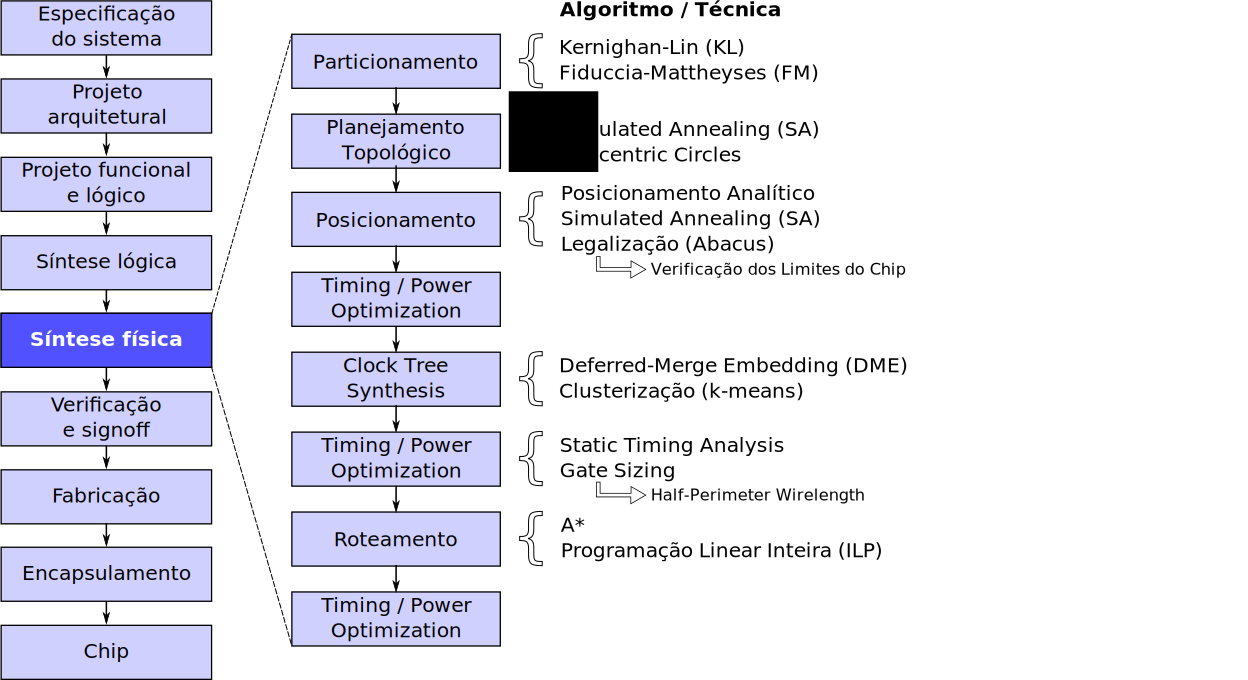
\includegraphics[width=\textwidth]{img/caracterizacao/exemplo_fluxo_com_algoritmos.pdf}
    \caption[Etapas da síntese física]{Etapas da síntese física com seus respectivos algoritmos/técnicas. Figura adaptada de~\citeonline{kahng2011vlsi}.}
    \label{fig:exemplo_fluxo_com_algoritmos}
\end{figure}

O Particionamento é a primeira etapa da síntese física e tem como objetivo dividir o \ac{ic} em sub-circuitos para minimizar o número de interconexões entre estas partições \cite{kahng2011vlsi}. Para resolver este problema de particionamento, existem dois algoritmos clássicos: Kernighan-Lin (KL)~\cite{kernighan1970efficient} e Fiduccia-Mattheyses (FM) \cite{fiduccia1988linear}.

% O algoritmo KL opera sobre uma representação do circuito modelada através de um grafo $G(V, E)$. Os nodos $e \in E$ deste grafo representam as células do circuito, enquanto, as arestas $v \in V$ modelam as conexões entre as células. Dado este grafo $G$, cujo $|V| = 2n$ e cada aresta $v$ possui o mesmo peso, o algoritmo KL particiona o conjunto de nodos $V$ em dois conjuntos disjuntos ($A$ e $B$) de mesmo tamanho, isto é, $|A| = |B| = n$.
% Para realizar este particionamento, o algoritmo KL realiza a troca de dois nodos $e_1 \in A$ e $e_2 \in B$ entre as partições com objetivo de minimizar o número de arestas intersectadas pelas partições. Após esta troca, os nodos ($e_1$ e $e_2$) são fixados para prevenir movimentos reversos.

% O algoritmo FM também opera sobre uma modelagem do circuito representada em grafo. Este algoritmo oferece melhorias significativas perante o algoritmo KL. Nele, as células podem ser movidas independentes entre as partições, o que facilita o particionamento de conjuntos de tamanhos distintos. O algoritmo FM utiliza a área da célula no cálculo do peso das arestas do grafo. Esta consideração leva a mover primeiro as células com menor área e visa reduzir a perturbação gerada pelo particionamento. A complexidade do algoritmo FM é $\mathcal{O}(|Pins|)$.

Os dois algoritmos (KL e FM) representam o circuito através de um grafo $G(V, E)$ , onde os nodos $v \in V$ representam as células e as arestas $e \in E$ modelam as conexões entre as células. Dado este grafo $G$, cujo $|V| = 2n$ e cada aresta $e$ possui o mesmo peso, o algoritmo KL particiona o conjunto de nodos $V$ em dois conjuntos disjuntos ($A$ e $B$) de mesmo tamanho, isto é, $|A| = |B| = n$.
Para realizar este particionamento, o algoritmo KL realiza a troca de dois nodos $v_1 \in A$ e $v_2 \in B$ entre as partições com objetivo de minimizar o número de arestas intersectadas pelas partições. Após esta troca, os nodos ($v_1$ e $v_2$) são fixados para prevenir movimentos reversos.
O algoritmo FM oferece melhorias significativas perante o algoritmo KL. Nele, uma única  célula pode ser movida entre as partições, o que facilita o particionamento de conjuntos de tamanhos distintos ($|A| \neq |B|$).
O algoritmo FM utiliza a área da célula no cálculo do peso das arestas do grafo. Esta consideração leva a mover primeiro as células com menor área e visa reduzir a perturbação gerada pelo particionamento. 
A complexidade do algoritmo FM é $\mathcal{O}(n)$, onde $n = |V|$, ao passo que, a complexidade do algoritmo KL é $\mathcal{O}(n^2~log~n)$, onde $n = |V|$.


Na etapa de planejamento topológico são definidas as localizações e formas dos módulos pertencentes ao circuito.
Com estas, é possível realizar estimativas precoces do tamanho das interconexões (\textit{wirelength}) e atraso. 
Esta análise inicial permite identificar quais blocos precisam de maior otimização nas etapas posteriores do fluxo de projeto de um \ac{ic}. 
A etapa de planejamento topológico é tipicamente dividida em três subetapas, que são elas: \textit{floorplanning}, \textit{pin assignment} e \textit{power planning}.
A subetapa de \textit{floorplanning} determina as localizações e dimensões, com base nas áreas e relações dos módulos, de modo a otimizar o tamanho do chip, reduzir as interconexões e melhorar a temporização do circuito. Para isso esta etapa avalia diferentes posicionamentos dos módulos pertencentes ao circuito.
O resultado final desta etapa pode ser observado na Figura~\ref{subfig:resultadofloorplan} onde a área total do \textit{chip} foi minimizada e possui $35$ unidades.
Um possível algoritmo para esta etapa é o Simulated Annealing (SA)~\cite{russell2009artificial}.

O algoritmo SA é iterativo - inicia com uma solução inicial ($s_i$) e busca incrementalmente melhorar a função objetivo $F$.
A cada iteração soluções vizinhas ($S_v$) são consideradas.
Estas soluções vizinhas são obtidas com uma pequena perturbação na solução atual ($S_v = s_a \pm \alpha$).
Para cada $s \in S_v$, se $s$ for melhor que a solução atual ($F(s) < F(s_a)$ assumindo um objetivo de minimização da função objetivo $F$) esta solução é tomada como solução atual ($s_a = s$).
Senão, existe uma probabilidade $t$ (temperatura) da solução $s$ ser tomada como solução atual. Esta probabilidade $t$ é reduzida a medida que o algoritmo executa, de forma que o mesmo sempre possui convergência para uma solução ótima local.
% Se esta probabilidade fosse infinitamente reduzida o algoritmo sempre encontraria o ótimo global, porém, isso não é verdade na prática.

\begin{figure}[h!t]
    \centering
    \subfigure[]{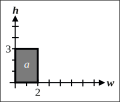
\includegraphics[width=0.3\textwidth]{img/caracterizacao/floorplan/floorplan.pdf} \label{subfig:resultadofloorplan}}
    \subfigure[]{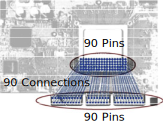
\includegraphics[width=0.3\textwidth]{img/caracterizacao/floorplan/pin_assignment.pdf} \label{subfig:resultadopinAssignment}}
    \subfigure[]{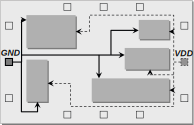
\includegraphics[width=0.32\textwidth]{img/caracterizacao/floorplan/power_planning.pdf} \label{subfig:resultadopowerPlanning}}
    
    \caption{Etapas do planejamento topológico. Retirado de \citeonline{kahng2011vlsi}.}
    \label{fig:etapasPlanejamentoTopologico}
\end{figure}

A subetapa de \textit{pin assignment} conecta as redes de sinais de saída do \ac{ic} com os pinos pertencentes aos blocos internos ao \ac{ic}.
O resultado final desta etapa pode ser observado na Figura~\ref{subfig:resultadopinAssignment}, sendo um dos principais algoritmos para esta etapa é o Concentric Circles \cite{koren1972pin, brady1984approach}.
A Figura~\ref{fig:concentricCircles} apresenta as principais etapas deste algoritmo.
Este algoritmo assume que todos os pinos externos (pinos fora do bloco atual) possuem localizações fixas (representados pelos círculos em verde na Figura~\ref{subfig:concentricCircles::a}). 
O algoritmo utiliza dois círculos concêntricos - o círculo interno mapeia os pinos do bloco atual (fontes dos sinais) enquanto, o círculo externo mapeia os pinos dos demais blocos conectados a este (destinos dos sinais).
Para cada pino é traçado uma linha do centro do círculo até sua posição, e sua posição é projetada para o respectivo círculo.
Este mapeamento pode ser observado pelos pontos em vermelho na Figura~\ref{subfig:concentricCircles::c}.
O mapeamento inicial é determinado por dado um pino fonte e um destino, interconecta-se estes pinos (linha trastejada da Figura~\ref{subfig:concentricCircles::d2}) e mapeia-se os demais pinos no sentido horário.
O mapeamento de todos os pinos pode ser observado na Figura~\ref{subfig:concentricCircles::g}.
Este processo é repetido para cada combinação de fonte/destino, sendo o melhor mapeamento determinado pela menor distância Euclidiana entre todos os fontes/destinos.
Neste exemplo o melhor mapeamento para os pinos é o demonstrado pela Figura~\ref{subfig:concentricCircles::e}.
Após determinar o mapeamento este algoritmo conecta os pinos do bloco atual (fontes dos sinais) com os pinos dos demais blocos conectados a este (destinos dos sinais), Este passo é ilustrado pela Figura~\ref{subfig:concentricCircles::f}.

\begin{figure}[h!t]
    \centering
    \subfigure[]{\includegraphics[width=0.3\textwidth]{img/caracterizacao/concentricCircles/a.pdf} \label{subfig:concentricCircles::a}}
    % \subfigure[]{\includegraphics[width=0.32\textwidth]{img/caracterizacao/concentricCircles/b.pdf} \label{subfig:concentricCircles::b}}
    \subfigure[]{\includegraphics[width=0.3\textwidth]{img/caracterizacao/concentricCircles/c.pdf} \label{subfig:concentricCircles::c}}
    \subfigure[]{\includegraphics[width=0.3\textwidth]{img/caracterizacao/concentricCircles/d2.pdf} \label{subfig:concentricCircles::d2}}
    
    \subfigure[]{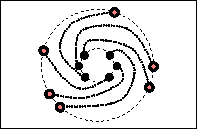
\includegraphics[width=0.3\textwidth]{img/caracterizacao/concentricCircles/g.pdf} \label{subfig:concentricCircles::g}}
    \subfigure[]{\includegraphics[width=0.3\textwidth]{img/caracterizacao/concentricCircles/e.pdf} \label{subfig:concentricCircles::e}}
    \subfigure[]{\includegraphics[width=0.3\textwidth]{img/caracterizacao/concentricCircles/f.pdf} \label{subfig:concentricCircles::f}}
    \caption[Ilustração algoritmo \textit{Concentric Circles}]{Exemplo da execução do algoritmo \textit{Concentric Circles}. Adaptado de \citeonline{kahng2011vlsi}.}
    \label{fig:concentricCircles}
\end{figure}

Na subetapa de \textit{power planning} constrói-se a rede de fornecimento de energia, isto é, redes de \textit{VDD} e \textit{ground}, de modo a assegurar que cada bloco é fornecido com a tensão de alimentação apropriada. A Figura~\ref{subfig:resultadopowerPlanning} apresenta o resultado desta etapa.

A etapa de posicionamento (\textit{placement}) é responsável por encontrar as posições e orientações de todos os elementos do circuito numa superfície planar.
Este posicionamento deve respeitar uma série de restrições (as células não podem se sobrepor uma as outras; todas as células devem estar alinhadas com as linhas e colunas do circuito; as células devem respeitar a linha de alimentação, sendo rotacionada quando necessário) e minimizar uma gama de objetivos (comprimento das interconexões, densidade do circuito).
Esta etapa de posicionamento é dividida em três subetapas: posicionamento global, legalização e posicionamento detalhado.
O posicionamento global negligencia algumas restrições (sobreposição e alinhamento das células) para simplificar o problema de posicionamento.
O principal objetivo nesta etapa é a redução das interconexões, mantendo a distribuição da densidade pelo circuito.
Para encontrar o local ideal de cada célula no circuito, utiliza-se técnicas analíticas para minimizar a função objetivo~\cite{tsay1988proud, eisenmann1998generic, Lin2013Polar}.
Outra técnica clássica de posicionamento global é baseada no algoritmo Simulated Annealing (SA). 

Como as técnicas de posicionamento global negligenciam algumas métricas, a etapa subsequente, denominada legalização, tem como propósito remover as sobreposições geradas pela etapa anterior.
Esta etapa também corrige as demais restrições impostas pela tecnologia, como por exemplo: alinhamento das células com a grade de alimentação, linhas e colunas do circuito.
Existem diversos algoritmos para a legalização de \acp{ic}, dentre eles um dos mais clássicos é o Abacus~\cite{spindler2008abacus}.
Abacus é um algoritmo de programação dinâmica que legaliza as células do circuito uma de cada vez, posicionando-as nas linhas que minimizam seu deslocamento com relação às posições encontradas pelo posicionamento global.

A etapa de legalização pode perturbar a solução encontrada pelo posicionamento global. Então, após a legalização é aplicada uma etapa de posicionamento detalhado.
Esta etapa reposiciona algumas células do circuito, otimizando métricas específicas, como por exemplo: atraso do circuito e densidade das células.
Para esta etapa são utilizados algoritmos iterativos que incrementalmente refinam o posicionamento das células críticas do circuito.

Com todas as células do circuitos posicionadas e legalizadas a etapa de \ac{cts} irá clusterizar elementos síncronos pertencentes ao mesmo sinal de relógio e planejar a rede de relógio do \ac{ic}.
Um dos algoritmos clássicos para o agrupamento de elementos pertencentes a mesma rede de relógio é denominado K-\textit{means}~\cite{selim1984k}.
O algoritmo inicia criando $k$ \textit{clusters} com centros aleatórios. Em seguida, na etapa de assinalamento, todos os elementos síncronos são assinalados para o \textit{cluster} mais próximo.
Após assinalar todos os elementos, o centro do \textit{cluster} é alterado para o centro de massa dos elementos que o pertencem. Estas duas etapas são repetidas por um número fixo de vezes ou até que os centros dos \textit{clusters} convirjam.

Para gerar a rede de relógio, dentre os algoritmos clássicos temos como exemplo o Deferred-Merge Embedding (DME)~\cite{boese1992zero}.
Este algoritmo é baseado no conceito de divisão e conquista e em tempo linear constrói a topologia de conexão no plano de Manhattan para criar uma árvore de relógio com \textit{clock skew} zero, minimizando o comprimento de fio das interconexões de relógio.
\textit{Clock Skew} é a máxima diferença no tempo de chegada (\textit{arrival time}) do sinal de relógio entre todos os elementos sequenciais. Se $t(u,v)$ representa o atraso na chegada do sinal de relógio entre os elementos sequenciais $u$ e $v$, o \textit{skew} de uma rede de relógio $T$ é calculado segundo a Equação \ref{eq.skew}.
\begin{equation} \label{eq.skew}
	 \displaystyle \operatorname{\textit{skew}(T)} = \max_{S_{i}, S_{j} \in S} | t(S_{0},S_{i})-t(S_{0},S_{j})|
%	 \displaystyle \operatorname{\textit{skew}(T)} = \max_{i,j \in S} | at_i^L - at_j^L|
\end{equation} 


Durante a etapa de roteamento todas as interconexões de sinais (\textit{nets}) devem ser estabelecidas. 
Esta etapa é subdividida em dois passos: 1) roteamento global; 2) roteamento detalhado.
No roteamento global, o circuito é dividido numa grade em que cada área desta grade é denominada gcell.
Cada gcell possui uma capacidade que representa o número de interconexões que podem ser roteadas nesta fração do circuito.
O modelo utilizado para representar estas informações de forma computacional é um Grafo G(V, E), em que os vértices $v \in V$ representam as gcell e as arestas $(u, v) \in E$ representam a capacidade da gcell $u$ rotear um sinal para a gcell vizinha $v$.
Então, para cada par de pinos interconectados são definidas as gcells em que a interconexão irá passar.
Um algoritmo capaz de definir por quais gcells a interconexão passa é o $A*$~\cite{russell2009artificial}.
Na etapa de roteamento detalhado, são definidas as trilhas de roteamento, vias e camadas de metais para cada segmento pertencente as interconexões do circuito.
Estas definições devem respeitar todas as regras de projetos estabelecidas para uma dada tecnologia de fabricação~\cite{kahng2011vlsi}.
Para isso, são definidas um conjunto de equações e estas são solucionadas por meio de \ac{ilp}.
Entre os roteadores clássicos baseados em \ac{ilp} estão Sidewinder~\cite{hu2008sidewinder} e BoxRouter~\cite{cho2007boxrouter}.


Durante todo o fluxo do \ac{ic}, a etapa de \textit{Timing/Power Optimization} é responsável por verificar se o circuito satisfaz as restrições de desempenho para uma frequência alvo de operação e aplicar otimizações incrementais.
Nesta etapa, a \ac{sta})~\cite{srivastava2006statistical, chadha2009static} propaga os atrasos das células e interconexões para identificar os locais com violações temporais.
Para isto, o circuito é modelado como um grafo G(V, E) em que os vértices $v \in V$ representam as células do circuito e as arestas $(u, v) \in E$ representam que a célula $u$ é interconectada com a célula $v$. 
Após identificar as violações temporais diferentes heurísticas são aplicadas para solucionar estas violações.
% Esta etapa é denominada \textit{Timing/Power Optimization} e possui dois grandes passos: \textit{Static Timing Analysis}~(STA)~\cite{srivastava2006statistical, chadha2009static} e \textit{Gate Sizing}.
% A análise consiste em propagar os atrasos das células e interconexões para identificar os locais com violações temporais.
% A etapa de \textit{Gate Sizing} é responsável por corrigir as violações temporais identificadas anteriormente.
% Estas correções são realizadas com a alteração do tamanho das células (uma biblioteca standard-cell tipicamente fornece a  mesma célula com diferentes tamanhos que correspondem a diferentes \textit{drive strengths}~\footnote{\textit{Drive strengths} é a quantidade de corrente que uma célula pode fornecer em seu chaveamento.}), a inserção de \textit{buffers} e a reestruturação da \textit{netlist}.

% sumarização da síntese física

A Tabela~\ref{tab:caracteristicasSinteseFisica} sintetiza as características das etapas da síntese física descrevendo os algoritmos/técnicas e suas estruturas de dados/métodos.
% Para cada etapa são descritos seus algoritmos e/ou técnicas bem como suas estruturas de dados e/ou métodos utilizados. 
Note que que diversos algoritmos/técnicas utilizam estruturas de dados elementares, como por exemplo: arranjos, pilhas, filas, conjuntos, entre outras.
Outra parcela destas etapas representa as informações do circuito por meio de um grafo.
Também existem etapas que fazem uso de outros métodos de programação, tais como: Programação Linear e Programação Dinâmica.

% Please add the following required packages to your document preamble:
% \usepackage{booktabs}
% \usepackage{multirow}
% \usepackage{graphicx}
\begin{table}[h!b]
\centering
\caption{Caracterização da Síntese Física}
\label{tab:caracteristicasSinteseFisica}
\resizebox{\textwidth}{!}{%
\begin{tabular}{@{}lll@{}}
\toprule
Etapa                                                                                  & Algoritmo / Técnica            & Estrutura de Dados / Método      \\ \midrule
\multirow{2}{*}{Particionamento}                                                       & Kernighan-Lin (KL)             & Grafo                            \\
                                                                                       & Fiduccia-Mattheyses (FM)       & Grafo                            \\ \midrule
\multirow{2}{*}{Planejamento Topológico}                                               & Simulated Annealing (SA)       & Elementar                        \\
                                                                                       & Concentric Circles             & Elementar                        \\ \midrule
\multirow{3}{*}{Posicionamento}                                                        & Posicionamento Analítico       & Programação Linear               \\
                                                                                       & Simulated Annealing (SA)       & Elementar                        \\
                                                                                       & Abacus                         & Programação Dinâmica             \\ \midrule
\multirow{2}{*}{\begin{tabular}[c]{@{}l@{}}Timing / Power\\ Optimization\end{tabular}} & Static Timing Analysis (STA)   & Grafo                            \\
                                                                                       & Gate Sizing                    & Grafo                            \\ \midrule
\multirow{2}{*}{Clock Tree Synthesis}                                                  & Deferred-Merge Embedding (DME) & Elementar                        \\
                                                                                       & K-means                        & Elementar                        \\ \midrule
\multirow{2}{*}{Roteamento}                                                            & A*                             & Grafo                            \\
                                                                                       & Sidewinder                     & Programação Linear Inteira (ILP) \\ \bottomrule
\end{tabular}%
}
\end{table}

% Please add the following required packages to your document preamble:
% \usepackage{multirow}
% \usepackage{graphicx}
% \begin{table}[]
% \centering
% \caption{Caracterização da Síntese Física}
% \label{tab:caracteristicasSinteseFisica}
% \resizebox{\textwidth}{!}{%
% \begin{tabular}{lll}
% \hline
% Etapa                                                                                  & Estratégia                     & Organização dos Dados            \\ \hline
% \multirow{2}{*}{Particionamento}                                                       & Kernighan-Lin (KL)             & Grafo                            \\
%                                                                                       & Fiduccia-Mattheyses (FM)       & Grafo                            \\ \hline
% \multirow{2}{*}{Planejamento Topológico}                                               & Simulated Annealing (SA)       &                                  \\
%                                                                                       & Concentric Circles             &                                  \\ \hline
% \multirow{3}{*}{Posicionamento}                                                        & Posicionamento Analítico       & Programação Linear               \\
%                                                                                       & Simulated Annealing (SA)       &                                  \\
%                                                                                       & Abacus                         & Programação Dinâmica             \\ \hline
% \multirow{2}{*}{\begin{tabular}[c]{@{}l@{}}Timing~/~Power Optimization\end{tabular}} & Static Timing Analysis (STA)   & Grafo                            \\
%                                                                                       & Gate Sizing                    & Grafo                            \\ \hline
% \multirow{2}{*}{Clock Tree Synthesis}                                                  & Deferred-Merge Embedding (DME) &                                  \\
%                                                                                       & K-means                        &                                  \\ \hline
% \multirow{2}{*}{Roteamento}                                                            & A*                             & Grafo                            \\
%                                                                                       & Sidewinder                     & Programação Linear Inteira (ILP) \\ \hline
% \end{tabular}%
% }
% \end{table}


% Please add the following required packages to your document preamble:
% \usepackage{booktabs}
% \usepackage{multirow}
% \usepackage{graphicx}
% \begin{table}[]
% \centering
% \caption{My caption}
% \label{my-label}
% \resizebox{\textwidth}{!}{%
% \begin{tabular}{@{}lll@{}}
% \toprule
% Etapa                                    & Estratégia                     & Organização dos Dados            \\ \midrule
% \multirow{2}{*}{Particionamento}         & Kernighan-Lin (KL)             & Grafo                            \\
%                                          & Fiduccia-Mattheyses (FM)       & Grafo                            \\ \midrule
% \multirow{2}{*}{Planejamento Topológico} & Simulated Annealing (SA)       &                                  \\
%                                          & Concentric Circles             &                                  \\ \midrule
% \multirow{3}{*}{Posicionamento}          & Posicionamento Analítico       & Programação Linear               \\
%                                          & Simulated Annealing (SA)       &                                  \\
%                                          & Abacus                         & Programação Dinâmica             \\ \midrule
% \multirow{2}{*}{Clock Tree Synthesis}    & Deferred-Merge Embedding (DME) &                                  \\
%                                          & K-means                        &                                  \\ \midrule
% \multirow{2}{*}{Roteamento}              & A*                             & Grafo                            \\
%                                          & Sidewinder                     & Programação Linear Inteira (ILP) \\ \midrule
% \multirow{2}{*}{Timing Closure}          & Static Timing Analysis (STA)   & Grafo                            \\
%                                          & Gate Sizing                    & Grafo                            \\ \toprule
% \end{tabular}%
% }
% \end{table}

Com isso é possível eleger um subconjunto de algoritmos/técnicas que representa as principais características do fluxo da síntese física de um \ac{ic}.
Para este trabalho os seguintes algoritmos/técnicas foram escolhidos para fornecer uma grande representatividade da síntese física:
\begin{itemize}
    \itemsep0em
    \item \textbf{Verificação dos limites do chip}: pertencente a etapa de legalização do posicionamento de um \ac{ic}. Este estudo de caso representa tarefas simples e com estruturas de dados elementares. Porém, estas são executadas inúmeras vezes durante o fluxo de projeto.
    \item \textbf{Estimativa do comprimento de interconexões}: pertencente as etapas de posicionamento e \textit{timming/power optimization}. Esta tarefa depende de diversas informações 
    tradicionalmente separadas em diversos módulos. Possui baixa intensidade aritmética e utiliza estrutura de dados elementares.
    \item \textbf{Clusterização de registradores}: Pertencente a etapa de \textit{Clock Tree Synthesis}. Esta tarefa necessita de poucas informações e utiliza estruturas de dados elementares. Porém, realiza um alto número de operações aritméticas. 
    \item \textbf{Roteamento de interconexões}: pertencente a etapa de roteamento do \ac{ic}. Esta tarefa opera sobre um grafo que representa o leiaute do circuito.
\end{itemize}

Não foram analisadas tarefas que utilizam Programação Linear pois grande parte do esforço concentra-se na solução de um sistema de equações matemáticas.
Estas equações são resolvidas por meio de solucionadores matemáticos externos, os quais, possuem como entrada estruturas de dados previamente definidas.
Isto, torna impossível aplicar outra organização (por exemplo \ac{dod}) nos dados internos destes solvedores.
Com isso, alterar a organização dos dados numa pequena parcela da tarefa provavelmente não surtiria efeito sobre o contexto global da tarefa.
Por limitação do escopo deste trabalho não foram analisadas tarefas que fazem uso de Programação Dinâmica.



% !TEX root = ../dissertacao.tex
\chapter{Resultados Experimentais}
\label{cap:resultados}

Este capítulo apresenta os resultados experimentais obtidos por este trabalho. 
Inicialmente, a Seção~\ref{sec:metodologia_experimental} descreve a metodologia adotada para avaliar os modelos de programação \ac{ood} e \ac{dod}.
A Seção~\ref{sec:infraestrutura_experimental} apresenta a infraestrutura experimental utilizada.
Por fim, as Seções~\ref{sec:estudo_de_caso_1} à \ref{sec:estudo_de_caso_4} apresentam um detalhamento de cada estudo de caso pertencente a síntese física.
Para cada estudo de caso é apresentado seu algoritmo, suas organizações de dados e realizada uma análise dos resultados experimentais obtidos.


\section{Metodologia Experimental}
\label{sec:metodologia_experimental}

Para quantizar o impacto da organização dos dados, foram avaliados o \textbf{número de  \textit{cache misses}} e o \textbf{tempo de execução} para cada estudo de caso definidos no Capítulo~\ref{cap:caracterizacaoSinteseFisica}.
Para os estudo de caso 1, 2, e 3 foram implementadas quatro versões: 1) utilizando o modelo \ac{ood} com execução sequencial; 2) utilizando o modelo \ac{dod} com execução sequencial; 3) utilizando o modelo \ac{ood} com execução paralelo; 4) utilizando o modelo \ac{dod} com execução paralela.
Para o estudo de caso 4 foram implementadas 2 versões: 1) utilizando o modelo \ac{ood} com execução sequencial; 2) utilizando o modelo \ac{dod} com execução sequencial.
Os experimentos podem apresentar resultados diferentes em cada execução, devido a interferências causadas pelo sistema operacional utilizado.
Portanto, para aumentar a confiança estatística obtida pelos experimentos, os mesmos foram repetidos 30 vezes, o que resultou em 99\% de confiança estatística\footnote{A confiança estatística foi medida utilizando o teste t de Student para p=0,01.}. Os resultados apresentados neste capítulo são as médias das 30 execuções.


\section{Infraestrutura e configuração experimental}
\label{sec:infraestrutura_experimental}

Os experimentos realizados utilizaram o conjunto de benchmarks disponibilizados pela competição \textit{ICCAD 2015 CAD Contest (problema C: Incremental Timing-Driven Placement)} \cite{kim2015}, o qual inclui 8 circuitos que possuem entre 768k e 1,93M células, todos derivados de circuitos industriais. Optou-se por utilizar tal infraestrutura pois a mesma disponibiliza circuitos com número de células compatível com circuitos contemporâneos. Além disso, tal infraestrutura é de acesso aberto, o que facilita a comparação experimental deste trabalho com trabalhos futuros. Como biblioteca básica, utilizou-se a Ophidian: Open-Source Library for Physical Design Research and Teaching~\cite{ophidian}.

Todas as implementações foram realizadas na linguagem $C++$ e compiladas com o compilador GCC 5.4.0. Para compilações com otimizações foram utilizadas as \textit{flags}: $O3$, ftree-vectorize e fopenmp. A \textit{flag} ftree-vectorize é responsável por habilitar a vetorização do código compilado, enquanto a \textit{flag} fopenmp é responsável pela paralelização do código com a biblioteca OpenMP~\cite{openmp}. Para medição do número de  \textit{cache misses} foi utilizado a ferramenta PAPI~\cite{papi} $5.6.0$.

Todos os experimentos foram executados em um computador com sistema operacional Debian GNU/Linux $8.2$ e processador Intel\textsuperscript{\textregistered} Core\textsuperscript{\textregistered} i5-4460 CPU @ 3.20~GHz.
A Figura~\ref{fig:architectureMemoryZeus} apresenta de forma gráfica a arquitetura deste computador.
Este computador possui 32GB RAM (DDR3 @ 1600MHz) como memória principal.
Seu processador possui quatro núcleos idênticos e três níveis de \textit{cache}.
Os primeiros dois níveis de \textit{cache}~(L1 and L2) são privativos para cada core do processador e possuem 64KB e 256KB de capacidade, respectivamente.
O terceiro nível de \textit{cache}~(L3) é compartilhado e possui 6144KB de capacidade.
Este processador possui $11$ contadores de \textit{hardware} o que possibiliza a ferramenta PAPI analisar os três níveis de \textit{cache} simultaneamente.

\begin{figure}[ht]
    \centering
    \includegraphics[width=0.5\linewidth]{img/results/architectureMemoryZeus.pdf}
    \caption{Arquitetura do computador utilizados nos experimentos.}
    \label{fig:architectureMemoryZeus}
\end{figure}


\section{Estudo de caso 1: Verificando os Limites do Chip}
\label{sec:estudo_de_caso_1}

Este estudo de caso visa avaliar um problema com baixa intensidade aritmética sobre um grande conjunto de dados.
Este problema consiste em verificar se cada célula do circuito está contida entre os limites físicos do \ac{ic} e é realizada na etapa de legalização do circuito.
Como a legalização é executada inúmeras vezes no fluxo de projeto é essencial que esta seja o mais otimizada possível.
Portanto, esta verificação pode impactar no desempenho da etapa de legalização pertencente a síntese física.

O Algoritmo~\ref{alg:problem1} descreve os passos a serem executados para verificar se todas as células estão posicionadas dentro dos limites de um chip.
Este Algoritmo recebe como entrada um conjunto de células $C$ e os limites do chip. 
Cada célula $c_i \in C$ possui sua localização representada por um ponto $(x(c_i), y(c_i))$.
Os limites do chip são representados por uma quádrupla ($\mathcal{X}_{min}$, $\mathcal{X}_{max}$ , $\mathcal{Y}_{min}$, $\mathcal{Y}_{max}$), onde $\mathcal{X}_{min}$ e  $\mathcal{Y}_{min}$ denotam os limites inferiores; e $\mathcal{X}_{max}$ e $\mathcal{Y}_{max}$ retratam os limites superiores.
Inicialmente uma variável que representa quantas células existem fora dos limites do chip é inicializada com zero (linha \ref{alg:problem1:var:initIlegal}).
Então, para cada célula $c_i$ do circuito (linhas \ref{alg:problem1:var:initFor} a \ref{alg:problem1:var:endFor}) é analisada se sua posição encontra-se fora dos limites (linhas \ref{alg:problem1:var:if}).
Se a posição de $c_i$ estiver além dos limites do chip a variável $ilegal$ é incrementada (linha \ref{alg:problem1:var:atribuicao}).
O número de células que estão fora dos limites do chip é retornado após percorrer todas as células (linha \ref{alg:problem1:var:retorno}).

\simbolo{$C$}{conjunto de células $C$ do circuito}
\simbolo{$c_i$}{i-ésima célula do conjunto $C$}
\simbolo{$x(c_i)$}{posição no eixo $x$ da célula $c_i$}
\simbolo{$y(c_i)$}{posição no eixo $y$ da célula $c_i$}

\begin{algorithm}[h!t]
	\SetKwInOut{Input}{Entrada}\SetKwInOut{Output}{Saída}
	\LinesNumbered
  	\Input{Conjunto de células $C$, Limites do Chip ($\mathcal{X}_{min}$, $\mathcal{X}_{max}$ , $\mathcal{Y}_{min}$, $\mathcal{Y}_{max}$) }
  	\Output{ Número de células além dos limites do chip }
    $ilegal \gets 0$\; \label{alg:problem1:var:initIlegal}
  	\ForEach{$c_i \in C$}{ \label{alg:problem1:var:initFor}
  	    \uIf{$(x(c_i) < \mathcal{X}_{min}) \lor (x(c_i) > \mathcal{X}_{max}) \lor$ $(y(c_i) < \mathcal{Y}_{min}) \lor (y(c_i) > \mathcal{Y}_{max})$}{ \label{alg:problem1:var:if}
  	       $ilegal \gets ilegal + 1$\; \label{alg:problem1:var:atribuicao}
  	    }
  	} \label{alg:problem1:var:endFor}
  	\Return $ilegal$\; \label{alg:problem1:var:retorno}
	\caption{Verificação dos Limites do Chip} 
	\label{alg:problem1}
\end{algorithm}

Na Figura~\ref{fig:problem1} estão representados dois exemplos de posicionamento de células em um circuito.
A única diferença entre estes posicionamentos (Figura~\ref{subfig:problem1_a} e  \ref{subfig:problem1_b}) é o posicionamento da célula $c_1$.
No posicionamento da Figura~\ref{subfig:problem1_a} a célula $c_1$ viola o limite inferior do chip ($\mathcal{X}_{min}$), o que torna necessário executar algoritmos de legalização sobre este posicionamento para que a célula $c_1$ seja relocada para uma posição válida e legal.

\begin{figure}[ht]
    \centering
    \subfigure[Circuito com células além do limite do chip.]{\includegraphics[width=0.33\linewidth]{img/results/problem1/problem1_a.pdf} \label{subfig:problem1_a}}
    \hspace{1cm}
    \subfigure[Circuito sem violação dos limites do chip.]{\includegraphics[width=0.33\linewidth]{img/results/problem1/problem1_b.pdf} \label{subfig:problem1_b}}
    \caption{Exemplo de posicionamento de células sobre um circuito.}
    \label{fig:problem1}
\end{figure}

\subsection{Modelagem dos Dados}

Para verificar se todas as células estão contidas dentro dos limites do chip são necessários três informações sobre o mesmo circuito: limites do chip, lista das células e a posição de cada célula.
Estas informações podem ser separadas em três módulos: \textit{Floorplan}, \textit{Netlist} e \textit{Placement}.
O módulo \textit{Floorplan} contém informações pertinentes a área do circuito, como limites do chip e tamanho das linhas e colunas.
O módulo \textit{Netlist}, por sua vez, representa as informações das interconexões e lista das células do circuito.
No módulo \textit{Placement} estão contidas informações do posicionamento e geometrias das células.
Portanto, é possível modelar o problema utilizando \ac{ood} com três classes: \textit{Floorplan::Floorplan, Netlist::Cell e Placement::Cell}.
A Figura~\ref{subfig:problem1ModelagemDados_OOD} apresenta graficamente o diagrama de classes para este paradigma de programação.
A seta entre as classes \textit{Cell} dos módulos \textit{Netlist} e \textit{Placement} representa uma relação de hierarquia, significando que a classe \textit{Cell} do módulo \textit{Placement} estende os atributos da classe \textit{Cell} do módulo \textit{Netlist}.

\begin{figure}[h!t]
    \centering
    \subfigure[Diagrama de classes para modelar o problema de verificação dos limites do chip segundo paradigma de programação \ac{ood}.]{\includegraphics[width=0.6\linewidth]{img/results/problem1/classHierarchyChipBoundariesOOD.pdf} \label{subfig:problem1ModelagemDados_OOD}}
    % \hspace{0.1cm}
    
    \subfigure[Modelagem dos dados para o problema de verificação dos limites do chip segundo paradigma de programação \ac{dod}.]{\includegraphics[width=0.9\linewidth]{img/results/problem1/chipBoundariesDOD.pdf} \label{subfig:problem1ModelagemDados_DOD}}
    \caption[Organização dos dados estudo de caso 1]{Comparativo da organização dos dados entre os modelos de programação OOD e DOD.}
    \label{fig:problem1ModelagemDados}
\end{figure}

Com esta abordagem dos dados, segundo o modelo \ac{ood}, pode-se perceber que existem atributos nos objetos que não serão utilizados por este problema (nome e pinos pertencentes a uma célula).
Porém, estes atributos irão ser recuperados juntamente com atributos úteis para o problema.
Este fator pode reduzir a localidade espacial do programa, por consequência, degradar o desempenho da aplicação de modo geral.

Adotando o paradigma de programação \ac{dod}, somente são necessárias duas informações: limites do chip e a posição de cada célula.
A Figura~\ref{subfig:problem1ModelagemDados_DOD} apresenta um possível modelo dos dados segundo este paradigma de programação.
A posição de todas as células são armazenadas contiguamente em um único vetor (\textit{Cells  Positions}), isso retira a necessidade do algoritmo possuir uma lista de todas as células pertencentes ao chip.
Neste modelo de dados, o laço presente na linha \ref{alg:problem1:var:initFor} do Algoritmo~\ref{alg:problem1} seria limitado a percorrer todos os dados contidos no vetor \textit{Cells  Positions}.
Esta abordagem fornece uma ampla localidade espacial para este algoritmo e também reduz o número de atributos necessários para a execução deste algoritmo.

\subsection{Avaliação}

A Figura~\ref{fig:problem1resultSequencial} apresenta os resultados da execução sequencial para a verificação dos limites do chip.
Na Figura~\ref{fig:missSequentialProblem1} são apresentados os números de  \textit{cache misses}, em escala logarítmica, (eixo Y) para cada circuito avaliado (eixo X). As barras amarelas representam o modelo de dados Orientado a Objetos (\ac{ood}). As barras azuis representam o modelo Orientado a Dados (\ac{dod}). O número total de  \textit{cache misses} para o \ac{dod} (de $87$ a $103$) foi, em média, cinco ordens de grandeza menor do que o atingido pelo modelo \ac{ood} (de $3M$ a $11M$). A redução no número de  \textit{cache misses} é proveniente diretamente da melhor organização dos dados em memória. Nesta organização, os dados de uma mesma propriedade (posição de uma determinada célula neste problema) estão armazenados contiguamente em memória. Portanto, ao ocorrer um miss na \textit{cache}, somente dados úteis são recuperados da memória principal. Assim, é realizado um melhor aproveitamento dos blocos de dados recuperados da memória principal para a \textit{cache}.
Outro fator importante é a vetorização do código gerado pelo compilador. Como o laço (linha \ref{alg:problem1:var:initFor} a \ref{alg:problem1:var:endFor} do Algoritmo~\ref{alg:problem1} para modelo \ac{dod}) acessa somente informações contidas em um vetor, o compilador consegue facilmente identificar esse comportamento e substituir as instruções padrões (\ac{sisd}) por instruções vetoriais (\ac{simd}).

\begin{figure}
    \centering
    \subfigure[Número de  \textit{cache misses}.]{\includegraphics[width=0.47\linewidth]{img/results/problem1/problem1_miss_sequential.pdf} \label{fig:missSequentialProblem1}}
    \subfigure[Tempo de execução.]{\includegraphics[width=0.47\linewidth]{img/results/problem1/problem1_runtime_sequential.pdf} \label{fig:runtimeSequentialProblem1}}
    \caption{Resultados experimentais para a execução sequencial do estudo de caso 1.}
    \label{fig:problem1resultSequencial}
\end{figure}

% \begin{figure}[ht]
%     \centering
%     \includegraphics[width=0.65\linewidth]{img/results/problem1/problem1_miss_sequential.pdf}
%     \caption[Cache misses do estudo de caso~1 sequencial.]{Número de cache misses resultantes dos dois protótipos de software do studo de caso~1 com execução sequencial.}
%     \label{fig:missSequentialProblem1}
% \end{figure}

A exploração da localidade dos dados reduz o tempo de acesso à memória principal, que representa o gargalo principal.  O impacto desta redução no tempo de execução pode ser observado na Figura~\ref{fig:runtimeSequentialProblem1}. Este gráfico, em escala logarítmica, retrata o tempo de execução (eixo Y) em nanosegundos para cada circuito avaliado (eixo X). Pode-se observar que a versão \ac{dod} executou mais rápido em todos os circuitos avaliados. Os tempos de execução da versão \ac{dod} foram entre $572ns$ e $743ns$, enquanto os tempos de execução de \ac{ood} foram entre $55ms$ e $174ms$.
Note que a implementação com \ac{dod} executou em \textbf{nanossegundos} ao invés de \textbf{milissegundos}, isto reflete em uma redução média de cinco ordens de grandeza.
Portanto, para o estudo de caso~1, a diferença relativa~\footnote{A diferença relativa foi calculada com a seguinte equação: $dr = \frac{(OOD - DOD)}{OOD}$, onde OOD e DOD representam a média da métrica avaliada (número de  \textit{cache misses} ou tempo de execução).} entre a modelagem dos dados com paradigma de programação \ac{ood} e \ac{dod} é em média $99.99\%$.

% \begin{figure}[ht]
%     \centering
%     \includegraphics[width=0.65\linewidth]{img/results/problem1/problem1_runtime_sequential.pdf}
%     \caption[Tempo de execução estudo de caso~1 sequencial]{Tempo de execução para o estudo de caso~1 com execução sequencial.}
%     \label{fig:runtimeSequentialProblem1}
% \end{figure}

O Algoritmo~\ref{alg:problem1paralelo} apresenta uma versão paralela do Algoritmo~\ref{alg:problem1}.
Neste algoritmo o conjunto de células é percorrido de forma simultânea por diferentes \textit{threads}.
Note que a variável $ilegal$ deve ser compartilhada entre todos os fluxos de execuções e pode ser escrita simultaneamente.
Para isso, a função $reduction$, da API OpenMP~\cite{openmp}, fornece a cada \textit{thread} uma cópia local da variável $ilegal$ e, ao final de todos os fluxos de execuções, sincroniza o valor da variável de forma exclusiva.


\begin{algorithm}[h!t]
	\SetKwInOut{Input}{Entrada}\SetKwInOut{Output}{Saída}
	\LinesNumbered
  	\Input{Conjunto de células $C$, Limites do Chip ($\mathcal{X}_{min}$, $\mathcal{X}_{max}$ , $\mathcal{Y}_{min}$, $\mathcal{Y}_{max}$) }
  	\Output{ Número de células além dos limites do chip }
    $ilegal \gets 0$\; \label{alg:problem1paralelo:var:initIlegal}
  	\textit{\textbf{\#pragma omp parallel for reduction(}}$+:ilegal$\textit{\textbf{)}} \hspace{20pt} \ForEach{$c_i \in C$}{ \label{alg:problem1paralelo:var:initFor}
  	    \uIf{$(x(c_i) < \mathcal{X}_{min}) \lor (x(c_i) > \mathcal{X}_{max}) \lor$ $(y(c_i) < \mathcal{Y}_{min}) \lor (y(c_i) > \mathcal{Y}_{max})$}{ \label{alg:problem1paralelo:var:if}
  	       $ilegal \gets ilegal + 1$\; \label{alg:problem1paralelo:var:atribuicao}
  	    }
  	} \label{alg:problem1paralelo:var:endFor}
  	\Return $ilegal$\; \label{alg:problem1paralelo:var:retorno}
	\caption{Verificação dos Limites do Chip em Paralelo} 
	\label{alg:problem1paralelo}
\end{algorithm}

A Figura~\ref{fig:problem1ExecParallel} apresenta os resultados obtidos com a execução paralela do estudo de caso~1.
Na esquerda (Figura~\ref{fig:problem1ExecParallelMiss}) é apresentado, em escala logarítmica, o número de  \textit{cache misses} (eixo Y) para cada circuito (eixo X).
O número de  \textit{cache misses} para o modelo \ac{ood} foi entre $1M$ a $6M$ enquanto, para o modelo \ac{dod} foi entre $83k$ a $202k$.
Esta redução foi, em média, de uma ordem de grandeza.
No lado direito (Figura~\ref{fig:problem1ExecParallelRuntime}) é apresentado, em escala logarítmica, o tempo de execução em nanossegundos (eixo Y) para cada circuito (eixo X).
O tempo de execução foi entre $26$ e $96$ milissegundos para o modelo \ac{ood}. Já o modelo \ac{dod} executou entre $0.76$ e $1.62$ milissegundos, o que gerou uma redução média de uma ordem de grandeza e uma diferença relativa de $9.85\%$.

\begin{figure}[ht]
    \centering
    \subfigure[Número de  \textit{cache misses}.]{\includegraphics[width=0.48\linewidth]{img/results/problem1/problem1_miss_parallel.pdf} \label{fig:problem1ExecParallelMiss}}
    \subfigure[Tempo de execução.]{\includegraphics[width=0.48\linewidth]{img/results/problem1/problem1_runtime_parallel.pdf} \label{fig:problem1ExecParallelRuntime}}
    \caption[Resultados do estudo de caso~1 com execução paralela.]{Resultados, em escala logarítmica, para execução paralela do estudo de caso~1.}
    \label{fig:problem1ExecParallel}
\end{figure}

Comparando as execuções sequencial e paralela, pode-se notar que houve uma redução no número de  \textit{cache misses} para a versão \ac{ood} e um \textit{speedup} médio de $1.95$ no tempo de execução.
Porém, houve um aumento significativo no número de  \textit{cache misses} (aumento de 4 ordens de grandeza) e tempo de execução para a versão \ac{dod} (\textit{speedup} médio de $0.0006$).
Este aumento se deve ao fato de que a tarefa, no modelo \ac{dod}, já possuía um alto desempenho e seu tempo de execução era extremamente baixo.
O sobrecusto de criação e sincronização das \textit{threads} foi muito superior ao próprio tempo da aplicação.
Portanto, a paralelização desta aplicação não apresentou ganhos significativos quando comparado com a versão sequencial.


% \begin{figure}[ht]
%     \centering
%     \includegraphics[width=0.65\linewidth]{img/results/problem1/problem1_miss_parallel.pdf}
%     \caption[Cache misses do Problema~1 paralelo.]{Número de cache misses resultantes dos dois protótipos de software do Problema~1 com execução paralela.}
%     \label{fig:missParallelProblem1}
% \end{figure}

% \begin{figure}[ht]
%     \centering
%     \includegraphics[width=0.65\linewidth]{img/results/problem1/problem1_runtime_parallel.pdf}
%     \caption[Tempo de execução Problema~1 paralelo]{Tempo de execução para o Problema~1 com execução paralela.}
%     \label{fig:runtimeParallelProblem1}
% \end{figure}









\section{Estudo de caso 2: Estimativa do Comprimento de Interconexões}
\label{sec:estudo_de_caso_2}

A proposta deste estudo de caso é avaliar uma tarefa de baixa intensidade aritmética porém, com necessidade de diversas propriedades de diferentes entidades.
A estimativa das interconexões, dentro da síntese física, é uma atividade utilizada por algoritmos de posicionamento e \textit{timing/power optimization}.
Exitem diversos métodos para estimar o comprimento de uma interconexão, dentre eles estão o \ac{rsmt} e \ac{hpwl}.
A \ac{rsmt} fornece estimativas de comprimento com um alto nível de precisão, porém possui complexidade computacional superior a do \ac{hpwl}.

O modelo é \ac{hpwl} comumente usado nas etapas iniciais da síntese física por possuir um tempo de execução linear ao número de pinos pertencentes a interconexão ($\mathcal{O}|Pins|$).
O comprimento de fio é estimado como a metade do perímetro do retângulo mínimo que contém todos os pinos pertencentes a uma determinada interconexão.
A Figura~\ref{fig:problem2} exemplifica uma interconexão entre 4 células e seus respectivos pinos.
Na Figura~\ref{fig:problem2_a} é apresentada a \ac{rsmt} para esta interconexão.
Ao passo que, na Figura~\ref{fig:problem2_b} é apresentada a estimativa \ac{hpwl} para a mesma interconexão.
Nesta, o retângulo mínimo que contem os quatro pinos possui perímetro de $18$ unidades. Portanto, o comprimento desta interconexão é estimado em $9$ unidades.

\begin{figure}[ht]
    \centering
    \subfigure[]{\includegraphics[width=0.25\linewidth]{img/results/problem2/problemaB_a.pdf} \label{fig:problem2_a}}
    \hspace{1cm}
    \subfigure[]{\includegraphics[width=0.25\linewidth]{img/results/problem2/problemaB_b.pdf} \label{fig:problem2_b}}
    \caption[Exemplo do cálculo de HPWL.]{Exemplo da estimativa do comprimento de uma interconexão de quatro pinos. Adaptada de \citeonline{kahng2011vlsi}.}
    \label{fig:problem2}
\end{figure}

O Algoritmo~\ref{alg:problem2} descreve o procedimento para o cálculo do \ac{hpwl} para todas as interconexões do \ac{ic}. 
Este algoritmo recebe como entrada um conjunto $N$ de todas as interconexões do \ac{ic} e retorna a estimativa do comprimento destas interconexões.
Inicialmente, a estimativa das interconexões ($hpwl$) é inicializada com zero (linha \ref{alg:problem2:var:inithpwl}).
Então, para cada interconexão $n_i$ pertencente ao conjunto $N$ é recuperado o conjunto $P$ de seus pinos (linha~\ref{alg:problem2:var:conjuntoPins}) e calculado o retângulo que encapsula todos os pinos pertencentes a este conjunto (linhas~\ref{alg:problem2:var:initForPins} a \ref{alg:problem2:var:endForPins}).
Por conseguinte, a estimativa das interconexões ($hpwl$) do circuito é acrescida da metade do perímetro deste retângulo (linha~\ref{alg:problem2paralelo:var:somaHpwl}).
Finalmente, a estimativa total das interconexões é retornada na linha~\ref{alg:problem2:var:retorno}.

\simbolo{$N$}{conjunto de interconexões $N$ do circuito}
\simbolo{$n_i$}{i-ésima interconexão do conjunto $N$}
\simbolo{$pins(n_i)$}{\\ pinos pertencentes a interconexão $n_i$}
\simbolo{$P$}{conjunto de pinos $P$ do circuito}
\simbolo{$p_j$}{j-ésimo pino do conjunto $P$}
\simbolo{$x(p_j)$}{posição no eixo $x$ do pino $p_j$}
\simbolo{$y(p_j)$}{posição no eixo $y$ do pino $p_j$}

\begin{algorithm}[h!t]
	\SetKwInOut{Input}{Entrada}\SetKwInOut{Output}{Saída}
	\LinesNumbered
  	\Input{Conjunto de Interconexões do circuito $N$}
  	\Output{ Estimativa das Interconexões }
    $hpwl \gets 0$\; \label{alg:problem2:var:inithpwl}
  	\ForEach{$n_i \in N$}{ \label{alg:problem2:var:initForNets}
  	    $P \gets pins(n_i)$\; \label{alg:problem2:var:conjuntoPins}
  	    $x_{min}, y_{min} \gets \infty$\; \label{alg:problem2:var:initMin}
  	    $x_{max}, y_{max} \gets -\infty$\; \label{alg:problem2:var:initMax}
  	    \ForEach{$p_j \in P$}{ \label{alg:problem2:var:initForPins}
  	        \uIf{$x(p_j) < x_{min}$}{\label{alg:problem2:var:ifXmin} $x_{min} \gets x(p_j)$\;}
  	        \uIf{$y(p_j) < y_{min}$}{\label{alg:problem2:var:ifYmin} $y_{min} \gets y(p_j)$\;}
  	        \uIf{$x(p_j) > x_{max}$}{\label{alg:problem2:var:ifXmax} $x_{max} \gets x(p_j)$\;}
  	        \uIf{$y(p_j) > y_{max}$}{\label{alg:problem2:var:ifYmax} $y_{max} \gets y(p_j)$\;}
  	    } \label{alg:problem2:var:endForPins}
  	    $hpwl \gets hpwl + (x_{max} - x_{min}) + (y_{max} - y_{min})$\; \label{alg:problem2:var:somaHpwl}
  	} \label{alg:problem2:var:endForNets}
  	\Return $hpwl$\; \label{alg:problem2:var:retorno}
	\caption{\textit{Half-Perimeter Wirelength} (HPWL)} 
	\label{alg:problem2}
\end{algorithm}

\subsection{Modelagem dos Dados}
\label{subsec:modelagemDadosProblem2}

Para estimar o comprimento das interconexões utilizando o modelo \ac{hpwl} são necessárias três informações básicas a respeito do \ac{ic}: conjunto das interconexões, conjunto dos pinos pertencentes a cada interconexão, e posição dos pinos.
Estas informações podem ser divididas em dois módulos: \textit{Netlist} e \textit{Placement}.
A Figura~\ref{fig:problem2ModelagemDados} apresenta de forma gráfica a organização dos dados para os modelos \ac{ood} e \ac{dod}.
Na Figura~\ref{subfig:problem2ModelagemDados_OOD} é apresentado o diagrama de classes para estimar uma interconexão seguindo o modelo de programação \ac{ood}.
Neste diagrama, a seta entre as classes \textit{Pin} dos módulos \textit{Netlist} e \textit{Placement} representa uma relação de hierarquia, ao passo que, a seta de ponta de diamante entre as classes \textit{Net} e \textit{Pin} representa  uma relação de agregação --- o que significa que a \textit{Net} (interconexão) possui referência para seus \textit{pins} (pinos) enquanto, os pinos possuem referência para sua interconexão.

Já para o modelo \ac{dod} serão necessários duas entidades (\textit{Nets} e \textit{Pins}) e duas propriedades (\textit{Net Pins} e \textit{Pins Position}), resultando em quatro vetores de informações. Estes vetores estão representados de forma gráfica na Figura~\ref{subfig:problem2ModelagemDados_DOD}.
Seguindo esta modelagem dos dados, o laço da linha~\ref{alg:problem2:var:initForNets} à \ref{alg:problem2:var:endForNets} do Algoritmo~\ref{alg:problem2:var:retorno} irá iterar sobre o vetor \textit{Nets} apresentado nesta figura. O conjunto de pinos $P$ acessado na linha~\ref{alg:problem2:var:conjuntoPins} será recuperado a partir do vetor \textit{Net Pins} deste modelo. Já o laço da linha~\ref{alg:problem2:var:initForPins} à \ref{alg:problem2:var:endForPins} irá percorrer o vetor \textit{Pins}.

\begin{figure}[ht]
    \centering
    % Diagrama de classes para modelar o problema de estimativa do comprimento de interconexões segundo paradigma de programação \ac{ood}.
    \subfigure[]{\includegraphics[width=0.3\linewidth]{img/results/problem2/classHierarchyOOD.pdf} \label{subfig:problem2ModelagemDados_OOD}}
    % \hspace{0.1cm}
    % Modelagem dos dados para o problema de estimativa do comprimento de interconexões segundo paradigma de programação \ac{dod}.
    \subfigure[]{\includegraphics[width=0.64\linewidth]{img/results/problem2/estimativa_interconection_dod_2.pdf} \label{subfig:problem2ModelagemDados_DOD}}
    \caption[Organização dos dados estudo de caso 2]{Comparativo da organização dos dados para estimativa de interconexões entre os paradigmas de programação OOD e DOD.}
    \label{fig:problem2ModelagemDados}
\end{figure}


\subsection{Avaliação}

A Figura \ref{fig:problem2resultSequencial} apresenta os resultados para o estudo de caso 2 com execução sequencial. As barras amarelas representam o modelo de dados Orientado a Objetos (\ac{ood}), enquanto que as barras azuis representam o modelo Orientado a Dados (\ac{dod}). A Figura~\ref{fig:missSequentialProblem2} apresenta o número de  \textit{cache misses} (eixo Y) para cada circuito (eixo X). O número de  \textit{cache misses} foi entre $8M$ e $20M$ para o modelo \ac{ood}, enquanto o modelo \ac{dod} obteve entre $26M$ e $72M$.
A Figura~\ref{fig:runtimeSequentialProblem2} retrata o tempo de execução em milissegundos (eixo Y) para cada circuito (eixo X).
O modelo \ac{ood} executou entre $91$ e $226$ milissegundos, enquanto o modelo \ac{dod} executou entre $354$ e $951$ milissegundos 

\begin{figure}[ht]
    \centering
    \subfigure[Número de  \textit{cache misses}.]{\includegraphics[width=0.47\linewidth]{img/results/problem2/problem2_miss_sequential.pdf} \label{fig:missSequentialProblem2}}
    % \hspace{1cm}
    \subfigure[Tempo de execução.]{\includegraphics[width=0.47\linewidth]{img/results/problem2/problem2_runtime_sequential.pdf} \label{fig:runtimeSequentialProblem2}}
    \caption[Resultados estudo de caso 2 com execução sequencial]{Resultados com execução sequencial.}
    \label{fig:problem2resultSequencial}
\end{figure}

% \begin{figure}[ht]
%     \centering
%     \includegraphics[width=0.65\linewidth]{img/results/problem2/problem2_miss_sequential.pdf}
%     \caption[Cache misses do Problema~2 sequencial.]{Número de cache misses resultantes dos dois protótipos de software do Problema~2 com execução sequencial.}
%     \label{fig:missSequentialProblem2}
% \end{figure}

% \begin{figure}[ht]
%     \centering
%     \includegraphics[width=0.65\linewidth]{img/results/problem2/problem2_runtime_sequential.pdf}
%     \caption[Tempo de execução Problema~2 sequencial]{Tempo de execução para o Problema~2 com execução sequencial.}
%     \label{fig:runtimeSequentialProblem2}
% \end{figure}

Nesta organização de dados, pode-se perceber que o modelo \ac{dod} resultou num número muito superior de  \textit{cache misses} do que o modelo \ac{ood}. Este número elevado de  \textit{cache misses} impactou diretamente no tempo total da execução do mesmo modelo.
Esta degradação no desempenho se deve ao fato de que a posição dos pinos no vetor \textit{Pins Positions} não reflete a ordem em que as interconexões serão percorridas (ordem do vetor \textit{Nets}). 
Este desalinhamento entre as ordens de visita aos vetores pode, no pior caso, levar a recuperação de um bloco da memória principal para cada pino pertencente a mesma interconexão.


O Algoritmo~\ref{alg:problem2paralelo} apresenta uma versão paralela para o Algoritmo~\ref{alg:problem2}.
Este algoritmo estima o comprimento de cada interconexão $n_i$ de modo paralelo. 
Esta abordagem pode sanar parcialmente o problema do desalinhamento no acesso ao vetor de posições de pinos, uma vez que um bloco recuperado da memória principal é compartilhado entre todas as unidades de processamento do computador.
Porém, este compartilhamento entre as unidades de processamento não pode ser garantido sem o conhecimento prévio da ordem em que as interconexões serão percorridas.

\begin{algorithm}[h!t]
	\SetKwInOut{Input}{Entrada}\SetKwInOut{Output}{Saída}
	\LinesNumbered
  	\Input{Conjunto de Interconexões do circuito $N$}
  	\Output{ Estimativa das Interconexões }
    $hpwl \gets 0$\; \label{alg:problem2paralelo:var:inithpwl}
  	\textit{\textbf{\#pragma omp parallel for reduction(}}$+:hpwl$\textit{\textbf{)}} \hspace{20pt} \ForEach{$n_i \in N$}{ \label{alg:problem2paralelo:var:initForNets}
  	    $P \gets pins(n_i)$\; \label{alg:problem2paralelo:var:conjuntoPins}
  	    $x_{min}, y_{min} \gets \infty$\; \label{alg:problem2paralelo:var:initMin}
  	    $x_{max}, y_{max} \gets -\infty$\; \label{alg:problem2paralelo:var:initMax}
  	    \ForEach{$p_j \in P$}{ \label{alg:problem2paralelo:var:initForPins}
  	        \uIf{$x(p_j) < x_{min}$}{\label{alg:problem2paralelo:var:ifXmin} $x_{min} \gets x(p_j)$\;}
  	        \uIf{$y(p_j) < y_{min}$}{\label{alg:problem2paralelo:var:ifYmin} $y_{min} \gets y(p_j)$\;}
  	        \uIf{$x(p_j) > x_{max}$}{\label{alg:problem2paralelo:var:ifXmax} $x_{max} \gets x(p_j)$\;}
  	        \uIf{$y(p_j) > y_{max}$}{\label{alg:problem2paralelo:var:ifYmax} $y_{max} \gets y(p_j)$\;}
  	    } \label{alg:problem2paralelo:var:endForPins}
  	    $hpwl \gets hpwl + (x_{max} - x_{min}) + (y_{max} - y_{min})$\; \label{alg:problem2paralelo:var:somaHpwl}
  	} \label{alg:problem2paralelo:var:endForNets}
  	\Return $hpwl$\; \label{alg:problem2paralelo:var:retorno}
	\caption{\textit{Half-Perimeter Wirelength} (HPWL) em Paralelo} 
	\label{alg:problem2paralelo}
\end{algorithm}

A Figura~\ref{fig:problem2resultParallel} apresenta os resultados da execução paralela para o estudo de caso 2.
As barras amarelas representam o modelo de dados Orientado a Objetos (\ac{ood}), enquanto, as barras azuis representam o modelo Orientado a Dados (\ac{dod}).
A esquerda, na Figura~\ref{fig:missParallelProblem2}, é apresentado o número de  \textit{cache misses} (eixo Y) para cada circuito avaliado (eixo X).
Na direita, Figura~\ref{fig:runtimeParallelProblem2}, é exibido o tempo de execução em milissegundos (eixo Y) para cada circuito (eixo X).

É possível observar que a versão paralela resultou numa redução significativa em ambas as métricas (número de  \textit{cache misses} e tempo de execução) para os dois modelos de programação. Esta redução foi mais significativa para o modelo \ac{dod}. Isto provavelmente se deve ao fato do compartilhamento de blocos recuperados da memória principal entre unidades de processamento. Contudo, mesmo com a paralelização do código, a diferença relativa entre as duas abordagens foi de $-157\%$ para o número de  \textit{cache misses} e de $-74\%$ no tempo de execução.

\begin{figure}[ht]
    \centering
    \subfigure[Número de  \textit{cache misses}.]{\includegraphics[width=0.47\linewidth]{img/results/problem2/problem2_miss_parallel.pdf} \label{fig:missParallelProblem2}}
    % \hspace{1cm}
    \subfigure[Tempo de execução.]{\includegraphics[width=0.47\linewidth]{img/results/problem2/problem2_runtime_parallel.pdf} \label{fig:runtimeParallelProblem2}}
    \caption[Resultados estudo de caso 2 com execução paralela]{Resultados com execução paralela.}
    \label{fig:problem2resultParallel}
\end{figure}

% \begin{figure}[ht]
%     \centering
%     \includegraphics[width=0.65\linewidth]{img/results/problem2/problem2_miss_parallel.pdf}
%     \caption[Cache misses do Problema~2 paralelo.]{Número de cache misses resultantes dos dois protótipos de software do Problema~2 com execução paralela.}
%     \label{fig:missParallelProblem2}
% \end{figure}

% \begin{figure}[ht]
%     \centering
%     \includegraphics[width=0.65\linewidth]{img/results/problem2/problem2_runtime_parallel.pdf}
%     \caption[Tempo de execução Problema~2 paralelo]{Tempo de execução para o Problema~2 com execução paralela.}
%     \label{fig:runtimeParallelProblem2}
% \end{figure}


% AGRUPANDO AS POSIÇÕES DOS PINOS



Uma forma de melhorar a localidade espacial da posição de cada pino pertencente à mesma interconexão é agrupar esta propriedade em relação as interconexões.
Isto pode ser feito replicando os dados e aplicando, uma única vez, um algoritmo de agrupamento. 
A Figura~\ref{fig:problem2Modelagem_DOD_grouped} apresenta uma possível organização dos dados para o modelo \ac{dod} com replicação das entidades pinos e suas respectivas posições. 
Note que a única alteração da organização dos dados apresentada na Figura~\ref{subfig:problem2ModelagemDados_DOD} é a adição de dois novos vetores: \textit{Pins Grouped} e \textit{Pins Position Grouped}.
O vetor \textit{Pins Grouped} foi agrupado com relação ao vetor \textit{Nets}, ou seja, os pinos pertencentes a cada interconexão estão armazenados de forma contígua neste vetor. Para refletir esse agrupamento, o vetor \textit{Pins Positions Grouped} também segue a mesma indexação do vetor \textit{Pins Grouped}.

\begin{figure}
    \centering
    \includegraphics[width=\linewidth]{img/results/problem2/estimativa_interconection_dod_grouped.pdf}
    \caption[Agrupamento dos dados para o estudo de caso 2]{Modelagem dos dados para o estudo de caso 2. Nesta modelagem os dados referentes aos pinos foram replicados para gerar uma cópia com o agrupamento de informações.}
    \label{fig:problem2Modelagem_DOD_grouped}
\end{figure}


As Figuras~\ref{fig:problem2resultSequencialordered}~e~\ref{fig:problem2resultParallelordered} apresentam os resultados desta organização dos dados (para o modelo \ac{dod}) para execução sequencial e paralela respectivamente. 
As barras amarelas representam o modelo de dados Orientado a Objetos (\ac{ood}), enquanto, as barras azuis representam o modelo Orientado a Dados (\ac{dod}).
Os dados presentes para o modelo \ac{ood} seguem a organização apresentada na Figura~\ref{subfig:problem2ModelagemDados_OOD} da Subseção~\ref{subsec:modelagemDadosProblem2}.
Analisando os resultados para a execução sequencial, é possível observar que o número de  \textit{cache misses} reduziu, em média, duas ordens de grandeza (de $1.53\times10^7$ para $5.83\times10^5$) para o modelo \ac{dod}. Com isso, a diferença relativa entre os modelos passou a ser de $85.31\%$. Este resultado demonstra que a organização dos dados, para o modelo \ac{dod}, inicialmente proposta na Subseção~\ref{subsec:modelagemDadosProblem2} gerou uma baixa localidade espacial nos vetores de pinos e suas posições.
Outro benefício gerado pelo agrupamento das informações foi a vetorização do código gerado pelo compilador. Na versão proposta na Subseção~\ref{subsec:modelagemDadosProblem2} somente instruções \ac{sisd} foram traduzidas do código fonte. Porém, com a organização dos dados proposta pela Figura~\ref{fig:problem2Modelagem_DOD_grouped}, o compilador gerou instruções \ac{simd} para este estudo de caso.

\begin{figure}[ht]
    \centering
    \subfigure[Número de  \textit{cache misses}.]{\includegraphics[width=0.47\linewidth]{img/results/problem2/problem2_miss_sequential_property_ordered.pdf} \label{fig:missSequentialProblem2ordered}}
    % \hspace{1cm}
    \subfigure[Tempo de execução.]{\includegraphics[width=0.47\linewidth]{img/results/problem2/problem2_runtime_sequential_property_ordered.pdf} \label{fig:runtimeSequentialProblem2ordered}}
    \caption{Resultados do estudo de caso 2 com execução sequencial e agrupamento de propriedades.}
    \label{fig:problem2resultSequencialordered}
\end{figure}

% \begin{figure}[ht]
%     \centering
%     \includegraphics[width=0.65\linewidth]{img/results/problem2/problem2_miss_sequential_property_ordered.pdf}
%     \caption[Cache misses do Problema~2 sequencial com ordenamento.]{Número de cache misses resultantes dos dois protótipos de software do Problema~2 com execução sequencial.}
%     \label{fig:missSequentialProblem2ordered}
% \end{figure}

% \begin{figure}[ht]
%     \centering
%     \includegraphics[width=0.65\linewidth]{img/results/problem2/problem2_runtime_sequential_property_ordered.pdf}
%     \caption[Tempo de execução Problema~2 sequencial com ordenamento.]{Tempo de execução para o Problema~2 com execução sequencial com ordenamento..}
%     \label{fig:runtimeSequentialProblem2ordered}
% \end{figure}

A Figura~\ref{fig:runtimeSequentialProblem2ordered} apresenta os resultados do tempo de execução. A escala desta figura foi alterada em relação a escala apresentada na Figura~\ref{fig:runtimeSequentialProblem2}. Esta alteração na escala fez-se necessária para ser possível visualizar os tempos de execução para o modelo \ac{dod}.
Comparando as duas execuções sequenciais, pode-se observar que o modelo \ac{dod} atingiu uma redução de uma ordem de grandeza e gerou uma diferença relativa entre as técnicas de $85\%$. 
Ou seja, o modelo \ac{dod} resulta em menos \textit{cache misses} do que \ac{ood} quando os dados estão agrupados de forma mais eficiente.
É importante observar que esse agrupamento não é possível de ser feito no modelo \ac{ood} porque a posição de cada pino é armazenada internamente ao objeto \textit{Placement::Pin}.
Com isso, não é possível manter diversos agrupamentos (um para cada necessidade de algoritmos) com o modelo \ac{ood}.


Na Figura~\ref{fig:problem2resultParallelordered} são apresentados os resultados para a execução paralela do estudo de caso 2.
É possível observar que a execução paralela com dados agrupados atingiu uma taxa de redução superior a taxa atingida pela paralelização sem agrupamento de informações.
Na Figura~\ref{fig:missParallelProblem2ordered} é apresentado o número de  \textit{cache misses} (eixo Y) para cada circuito avaliado (eixo X).
O modelo \ac{ood} gerou entre $3M$ e $9M$ de \textit{cache misses}, tendo em média $5$ milhões de  \textit{cache misses} para cada circuito.
Já o modelo \ac{dod} provocou entre $374k$ e $1M$ de \textit{cache misses}, tendo em média $583$ mil  \textit{cache misses} para cada circuito. 
A diferença relativa entre os dois modelos foi, em média, de $90\%$.

Na Figura~\ref{fig:runtimeParallelProblem2ordered} estão apresentados os tempos de execução da execução paralela (eixo Y) em milissegundos para cada circuito avaliado (eixo X).
Os tempos de execução foram de $78ms$ a $193ms$ para o modelo \ac{ood} e de $4ms$ a $10ms$ para o modelo \ac{dod}.





\begin{figure}[ht]
    \centering
    \subfigure[Número de  \textit{cache misses}.]{\includegraphics[width=0.47\linewidth]{img/results/problem2/problem2_miss_parallel_property_ordered.pdf} \label{fig:missParallelProblem2ordered}}
    % \hspace{1cm}
    \subfigure[Tempo de execução.]{\includegraphics[width=0.47\linewidth]{img/results/problem2/problem2_runtime_parallel_property_ordered.pdf} \label{fig:runtimeParallelProblem2ordered}}
    \caption{Resultados do estudo de caso 2 com execução paralela e agrupamento de propriedades.}
    \label{fig:problem2resultParallelordered}
\end{figure}

% \begin{figure}[ht]
%     \centering
%     \includegraphics[width=0.65\linewidth]{img/results/problem2/problem2_miss_parallel_property_ordered.pdf}
%     \caption[Cache misses do Problema~2 paralelo com ordenamento..]{Número de cache misses resultantes dos dois protótipos de software do Problema~2 com execução paralela com ordenamento.}
%     \label{fig:missParallelProblem2ordered}
% \end{figure}

% \begin{figure}[ht]
%     \centering
%     \includegraphics[width=0.65\linewidth]{img/results/problem2/problem2_runtime_parallel_property_ordered.pdf}
%     \caption[Tempo de execução Problema~2 paralelo com ordenamento.]{Tempo de execução para o Problema~2 com execução paralela com ordenamento.}
%     \label{fig:runtimeParallelProblem2ordered}
% \end{figure}




\section{Estudo de caso 3: Clusterização de Registradores}
\label{sec:estudo_de_caso_3}

Este estudo de caso avalia uma tarefa com maior intensidade aritmética e com poucas propriedades.
Durante a etapa de \textit{Clock Tree Synthesis} os registradores próximos são agrupados para que um \textit{buffer} do sinal de relógio possa ser inserido. Este processo é denominado clusterização dos registradores. Dado um conjunto de posições dos registradores $\mathcal{R} = \{r_1, r_2, ..., r_n\}$ onde cada $r_i \in \mathbb{R}^2$, o problema de clusterizar os registradores pode ser definido como: particionar o conjunto $\mathcal{R}$ num número predefinido $k$ de \textit{clusters} $\Gamma = \{\gamma_1, \gamma_2, ..., \gamma_k\}$ onde a soma das interconexões pertencentes a cada \textit{cluster} seja minimizada. A soma das interconexões estão descritas nas Equações \eqref{eq:register_clustering} à \eqref{eq:union_constraint}.
Cada $\gamma_i \in \Gamma$ representa o conjunto de elementos pertencentes ao \textit{cluster} $i$.
A Equação~\eqref{eq:register_clustering} apresenta a função objetivo definida pela soma das distâncias Manhattan entre o centro de cluster $c_i$ e os elementos pertencentes a este cluster.
Geralmente, o centro do cluster é determinado pelo centro gravitacional de seus elementos: $c_i = \sum_{r_j \in \gamma_i} r_j/|\gamma_i|$, onde $|\gamma_i|$ representa o tamanho  de $\gamma_i$.
O conjunto de Equações \eqref{eq:empty_constraint} a \eqref{eq:union_constraint} definem as partições de $\mathcal{R}$, isto é, cada registrador deve pertencer a um, e exclusivamente um, \textit{cluster}.

\simbolo{$\mathcal{R}$}{conjunto de registradores $\mathcal{R}$ do circuito}
\simbolo{$\Gamma$}{conjunto de \textit{clusters} do circuito}
\simbolo{$\gamma_i$}{i-ésimo \textit{clister} do conjunto $\Gamma$}

\begin{eqnarray}
\label{eq:register_clustering}
    \textbf{Min}&:& \sum_{i = 1}^{k}\sum_{r_j \in \gamma_i} \lVert c_i - r_j\rVert_2^2 \\
    % \label{eq:cluster_mean}
    % && x_{cl_i} = \frac{\sum_{r_j \in cl_i} x_{r_j}}{|cl_i|}, \ y_{cl_i} = \frac{\sum_{r_j \in cl_i} y_{r_j}}{|cl_i|} \\
    \label{eq:empty_constraint}
    \textbf{S.t.} &:& \gamma_i \in \Gamma \implies \gamma_i \neq \emptyset \\
    \label{eq:intersection_constraint}
    &:&\gamma_i, \gamma_j \in \Gamma \ \land \ i \neq j \implies \gamma_i \cap \gamma_j = \emptyset\\
    \label{eq:union_constraint}
    &:& \mathcal{R} = \bigcup_{\gamma_i \in \Gamma} \gamma_i 
\end{eqnarray}

Um algoritmo clássico de clusterização de elementos é o \textit{K-means} \cite{selim1984k}.
Este algoritmo não é somente utilizado para clusterização de registradores, mas também em diferentes áreas como \textit{machine learning} e \textit{data mining}.
O Algoritmo~\ref{alg:problem3} descreve as etapas do algoritmo \textit{k-means}.
Este algoritmo recebe como entrada um conjunto $\mathcal{R}$ de posições de registradores e um conjunto $\mathcal{C}$ dos $k$ centros de \textit{clusters}.
Existem diversas formas de determinar o número $k$ de \textit{clusters}, neste trabalho o número máximo de elementos por \textit{cluster} foi limitado a $50$.
Portanto, o número $k$ de cluster para cada circuito foi determinado pelo número de registradores dividido por $50$ ($k=\lceil\frac{|\mathcal{R}|}{50}\rceil$).
A posição de cada centro de \textit{cluster} foi inicializada aleatoriamente com uma distribuição uniforme.
O retorno do algoritmo é um conjunto de \textit{clusters} e seus novos centros.

\begin{algorithm}[bht]
\SetKwInOut{Input}{Entrada}\SetKwInOut{Output}{Saída}
\SetKwRepeat{Do}{do}{while}
\LinesNumbered
     \Input{Conjunto $\mathcal{R}$ de posições dos registradores, conjunto $\mathcal{C}$ dos $k$ centros de clusters} 
     \Output{Conjunto de clusters $\Gamma$ e seus respectivos centros $\mathcal{C}$}
     \Do{centros dos clusters não convergirem}{
        $\gamma_i \gets \emptyset, \ i = 1 \dots k$\; \label{line:clear}
        \ForEach{$r_i \in \mathcal{R}$}{ \label{line:for_assignment_init}
            $c_j \gets \argmin_{c_j \in \mathcal{C}} \{\lVert c_j - r_i\rVert_2^2  \}$\; \label{alg:problem3:buscaRTree}
            $\gamma_j \gets \gamma_j \cup \{r_i\}$\;
        } \label{line:for_assignment_end}
        % $\Gamma \gets \bigcup_{i = 1}^k \gamma_i$\;
        \ForEach{$\gamma_i \in \Gamma$}{
            $c_i \gets \sum_{r_j \in \gamma_i} r_j/|\gamma_i|$\;
        }
     }
  \caption{\textit{K-means}} \label{alg:problem3}
\end{algorithm}

Inicialmente todos os \textit{clusters} estão vazios (line~\ref{line:clear}).
Então, o algoritmo resolve o problema da clusterização de registradores executando duas etapas principais: \textbf{assinalamento} e \textbf{atualização}.
Durante a etapa de assinalamento (linhas 3 a 6), cada registrador é assinalado para o centro de \textit{cluster} mais próximo da  sua posição.
Após assinalar todos os registradores para um cluster, na etapa de atualização (linhas 7 a 9), os centros dos \textit{clusters} são realocados para o centro de massa de seus elementos.
Estas duas etapas são executadas até que todos os centros dos \textit{clusters} convirjam ou limitadas por um número fixo de iterações.
Neste trabalho o número de iterações foi limitado a 10 e utilizou-se a mesma semente na geração das posições iniciais aleatórias dos centros dos \textit{clusters}.

% \begin{figure}[ht]
%     \centering
%     \includegraphics[width=0.3\linewidth]{img/results/problem3/problem3.pdf}
%     \caption[]{}
%     \label{fig:problem3}
% \end{figure}


\subsection{Modelagem dos Dados}
\label{subsec:modelagemDadosProblem3}
A Figura~\ref{fig:problem3ModelagemDados} apresenta uma possível modelagem dos dados para este estudo de caso.
A Figura~\ref{subfig:problem3ModelagemDados_OOD} ilustra o diagrama de classes para o modelo \ac{ood}.
Neste modelo são definidas duas classes: \textit{cluster} e \textit{Register}.
A seta de ponta de diamante entre estas classes representa  uma relação de agregação --- o que significa que o \textit{Cluster} possui referência para seus registradores.
Na Figura~\ref{subfig:problem3ModelagemDados_DOD} é possível observar a organização dos dados para o modelo \ac{dod}.
A Agregação representada pela seta de ponta de diamante entre estas classes no modelo \ac{ood} é neste caso realizada pelo vetor \textit{Cluster Registers}.
Também é possível observar que nesta abordagem não existem dados desnecessários (como o nome de um registrador) para o presente estudo de caso.

\begin{figure}[ht]
    \centering
    % Diagrama de classes para modelar a clusterização de registradores segundo paradigma de programação \ac{ood}.
    \subfigure[]{\includegraphics[width=0.35\linewidth]{img/results/problem3/problem3_OOD.pdf} \label{subfig:problem3ModelagemDados_OOD}}
    \hspace{0.1cm}
    % Modelagem dos dados para o problema de clusterizar os registradores segundo paradigma de programação \ac{dod}.
    \subfigure[]{\includegraphics[width=0.55\linewidth]{img/results/problem3/problem3_DOD.pdf} \label{subfig:problem3ModelagemDados_DOD}}
    \caption[Organização dos dados estudo de caso 3]{Comparativo da organização dos dados para estimativa de interconexões entre os paradigmas de programação OOD e DOD para o estudo de caso 3.}
    \label{fig:problem3ModelagemDados}
\end{figure}


\subsection{Avaliação}

A Figura~\ref{fig:resultsProblem3sequential} apresenta os resultados da execução sequencial do estudo de caso 3 utilizando a modelagem dos dados descrita na Seção~\ref{subsec:modelagemDadosProblem3}. 
As barras amarelas representam o modelo de dados Orientado a Objetos (\ac{ood}), enquanto, as barras azuis representam o modelo Orientado a Dados (\ac{dod}).
Na esquerda, Figura~\ref{fig:missSequentialProblem3}, o número de  \textit{cache misses} (eixo Y) para cada circuito avaliado (eixo X).
É possível observar que ambos os modelos (\ac{ood} e \ac{dod}) necessitaram de um número muito similar de  \textit{cache misses} para carregarem os dados para este estudo de caso.
Portanto, não é possível inferir informações estatísticas sobre os circuitos \textit{superblue4}, \textit{superblue5} e \textit{superblue1} pois nestes casos há uma intersecção no intervalo de confiança entre os dois modelos. Nos demais circuitos o modelo \ac{dod} obteve um desempenho ligeiramente melhor do que o modelo \ac{ood}.
A Figura~\ref{fig:runtimeSequentialProblem3} apresenta o tempo de execução em segundos (eixo Y) para cada circuito avaliado (eixo X).
Novamente, pode-se observar que existem intersecções nos intervalos de confiança.
Portanto, não é possível estimar qual dos dois modelos obteve um melhor desempenho.

\begin{figure}[hbt]
    \centering
    \subfigure[Número de  \textit{cache misses}.]{\includegraphics[width=0.47\linewidth]{img/results/problem3/problem3_miss_sequential.pdf} \label{fig:missSequentialProblem3}}
    \subfigure[Tempo de execução.]{\includegraphics[width=0.47\linewidth]{img/results/problem3/problem3_runtime_sequential.pdf} \label{fig:runtimeSequentialProblem3}}
    \caption{Resultados para a execução sequencial do estudo de caso 3.}
    \label{fig:resultsProblem3sequential}
\end{figure}

Uma possível explicação para o comportamento similar entre os dois modelos é o fato de que a busca espacial pelo centro do \textit{cluster} mais próximo a cada registrador foi realizado utilizando a estrutura de dados \textit{R-Tree}~\footnote{A estrutura de dados R-tree consiste em uma árvore espacial especializada no armazenamento de dados multidimensionais.}~\cite{manolopoulos2010r} para ambos os modelos.
Esta busca é realizada na linha~\ref{alg:problem3:buscaRTree} do Algoritmo~\ref{alg:problem3}. 
% O modelo \ac{dod} foi incapaz de atingir um alto desempenho na localidade espacial dos dados fornecidos a R-tree pois a alta intensidade aritmética esta concentrada exatamente na etapa de busca espacial e o acesso ao vetor das posições dos registradores não é garantidamente contíguo.
% Uma abordagem seria aplicar um agrupamento nas posições dos registradores pertencentes ao mesmo cluster. Isso daria garantias a localidade espacial dos dados na busca espacial.
% Porém, como um determinado registrador pode ser trocado de um \textit{cluster} para outro em cada iteração do algoritmo, seria necessário reagrupar o vetor de posições de registradores a cada iteração do algoritmo. Este sobrecusto de agrupar o vetor possivelmente é maior do que o custo gerado sem nenhum agrupamento/ordenamento dos dados.
O modelo \ac{dod} foi incapaz de atingir um alto desempenho pois a maior complexidade do algoritmo \textit{K-means} reside na busca espacial pelos \textit{clusters} próximos, que é realizada pela \textit{R-tree}, cuja estrutura interna independe da organização dos dados.

% \begin{figure}[ht]
%     \centering
%     \includegraphics[width=0.65\linewidth]{img/results/problem3/problem3_miss_sequential.pdf}
%     \caption[Cache misses do Problema~3 sequencial.]{Número de cache misses resultantes dos dois protótipos de software do Problema~3 com execução sequencial.}
%     \label{fig:missSequentialProblem3}
% \end{figure}

% \begin{figure}[ht]
%     \centering
%     \includegraphics[width=0.65\linewidth]{img/results/problem3/problem3_runtime_sequential.pdf}
%     \caption[Tempo de execução Problema~3 sequencial]{Tempo de execução para o Problema~3 com execução sequencial.}
%     \label{fig:runtimeSequentialProblem3}
% \end{figure}

O Algoritmo~\ref{alg:problem3parallel} apresenta uma versão paralela para o Algoritmo~\ref{alg:problem3}.
Ao paralelizar a etapa de assinalamento, linhas 4 a 6 do Algoritmo~\ref{alg:problem3}, é obrigatório a adição de um mapeamento extra para o conjunto de registradores pertencentes a cada \textit{cluster} (linha 5 do Algoritmo~\ref{alg:problem3}). Isto se faz necessário pois dois registradores podem escrever simultaneamente no mesmo \textit{cluster}.
Este mapeamento é realizado com um vetor auxiliar $\alpha$ de tamanho igual ao número de registradores do circuito --- $|\alpha| = |\mathcal{R}|$.
Então, na linha 5 do Algoritmo~\ref{alg:problem3parallel}, cada registrador irá escrever numa posição única do vetor $\alpha$ retirando assim a concorrência no acesso aos \textit{clusters}.
Com este mapeamento extra, é necessário adicionar um laço para atualizar as referências dos registradores pertencentes a um \textit{cluster}.
Isto é realizado entre as linhas 7 e 10 do Algoritmo~\ref{alg:problem3parallel}.
Ao paralelizar a etapa de atualização dos \textit{clusters}, linhas  7 a 9 do Algoritmo~\ref{alg:problem3}, não se faz necessária nenhuma alteração no código fonte uma vez que cada cluster irá escrever em variáveis distintas.

\begin{algorithm}[h!t]
\SetKwInOut{Input}{Entrada}\SetKwInOut{Output}{Saída}
\SetKwRepeat{Do}{do}{while}
\LinesNumbered
     \Input{Conjunto $\mathcal{R}$ de posições dos registradores, conjunto $\mathcal{C}$ dos $k$ centros de clusters} 
     \Output{Conjunto de clusters $\Gamma$ e seus respectivos centros $\mathcal{C}$}
     \Do{centros dos clusters não convergirem}{
        $\gamma_i \gets \emptyset, \ i = 1 \dots k$\;
        % $\alpha \gets \emptyset, \ i = 1 \dots k$\;
        \textit{\textbf{\#pragma omp parallel for}} \hspace{75pt} \ForEach{$r_i \in \mathcal{R}$}{
            $c_j \gets \argmin_{c_j \in \mathcal{C}}\{\lVert c_j - r_i\rVert_2^2 \}$\;
            $\alpha_i \gets \gamma_j$\;
        }
        
        \ForEach{$r_i \in \mathcal{R}$}{        
            $\gamma_j \gets \alpha_i$\;
            $\gamma_j \gets \gamma_j \cup \{r_i\}$\;
        }
        
        % $\Gamma \gets \bigcup_{i = 1}^k \gamma_i$\;
        \textit{\textbf{\#pragma omp parallel for}} \hspace{75pt} \ForEach{$\gamma_i \in \Gamma$}{
            $c_i \gets \sum_{r_j \in \gamma_i} r_j/|\gamma_i|$\;
        }
     }
  \caption{\textit{K-means} em paralelo}
  \label{alg:problem3parallel}
\end{algorithm}



\begin{figure}[h!b]
    \centering
    \subfigure[Número de  \textit{cache misses}.]{\includegraphics[width=0.47\linewidth]{img/results/problem3/problem3_miss_parallel.pdf} \label{fig:missParallelProblem3}}
    \subfigure[Tempo de execução.]{\includegraphics[width=0.47\linewidth]{img/results/problem3/problem3_runtime_parallel.pdf} \label{fig:runtimeParallelProblem3}}
    \caption{Resultados para a execução paralela do estudo de caso 3.}
    \label{fig:resultsProblem3parallel}
\end{figure}

A Figura~\ref{fig:resultsProblem3parallel} apresenta os resultados da execução paralela do estudo de caso 3.
As barras amarelas representam o modelo de dados Orientado a Objetos (\ac{ood}) enquanto, as barras azuis representam o modelo Orientado a Dados (\ac{dod}).
É possível observar que, ao paralelizar o algoritmo k-means, o modelo \ac{dod} favoreceu a localidade espacial e reduziu o número de  \textit{cache misses} da maioria dos circuitos.
O número de  \textit{cache misses} para o modelo \ac{ood} foi em média $9.49M$, com coeficiente de variação\footnote{O coeficiente de variação $cv$ é definido como $cv = \frac{\sigma}{\mu}$ onde $\sigma$ e $\mu$ representam respectivamente o desvio padrão e a média.} médio de $13\%$.
Para o modelo \ac{dod}, o número de  \textit{cache misses} foi em média $6.49M$, e teve um coeficiente de variação de $10\%$.



% \begin{figure}[ht]
%     \centering
%     \includegraphics[width=0.65\linewidth]{img/results/problem3/problem3_miss_parallel.pdf}
%     \caption[Cache misses do Problema~3 paralelo.]{Número de cache misses resultantes dos dois protótipos de software do Problema~3 com execução paralela.}
%     \label{fig:missParallelProblem3}
% \end{figure}

% \begin{figure}[ht]
%     \centering
%     \includegraphics[width=0.65\linewidth]{img/results/problem3/problem3_runtime_parallel.pdf}
%     \caption[Tempo de execução Problema~3 paralelo]{Tempo de execução para o Problema~3 com execução paralela.}
%     \label{fig:runtimeParallelProblem3}
% \end{figure}

A Figura~\ref{fig:runtimeParallelProblem3} apresenta os tempos de execução (eixo Y), em segundos, para cada circuito avaliado (eixo X).
O modelo \ac{dod} foi mais rápido que o modelo \ac{ood} em todos os circuitos avaliados.
O modelo \ac{ood} executou entre $0.20$ (no circuito \textit{superblue18}) e $0.44$ (no circuito \textit{superblue10}) segundos, em média este modelo levou $0.32$ segundos com desvio padrão médio de $2.77\%$ em relação a média das execuções. 
Já o modelo \ac{dod} executou entre $0.16$ (no circuito \textit{superblue5}) e $0.43$ (no circuito \textit{superblue7}) segundos, com média de $0.29$ segundos e desvio padrão médio de $3.28\%$ em relação a média das execuções.
A diferença relativa entre as duas técnicas foi de $8.75\%$, o que sugere que a implementação dod oferece mais potencial de paralelismo neste problema.




\section{Estudo de caso 4: Roteamento de Interconexões}
\label{sec:estudo_de_caso_4}

Este estudo de caso avalia tarefas que possuem suas informações representadas por meio de um grafo.
Durante a etapa de síntese física de um \ac{ic}, a etapa de roteamento global é responsável por interconectar os pinos pertencentes a um mesmo potencial elétrico.
Durante esta etapa, o leiaute do circuito é representado por regiões de roteamento denominadas $gcell$.
A Figura~\ref{subfig:problem4_a} apresenta de forma gráfica a subdivisão do leiaute do circuito nas $gcell$.
Todas as interconexões do circuito devem ser minimizadas para otimizar o comprimento total das interconexões do circuito e/ou otimizar outros objetivos~\cite{kahng2011vlsi}.
Uma heurística utilizada para minimizar o roteamento global é a distância Manhattan entre os pontos a serem conectados.
Na Figura~\ref{subfig:problem4_a} esta distância é representada pela heurística $h(A, B)$, onde as $gcell$ $A$ e $B$ estão distantes $9$ unidades.


\begin{figure}[h!t]
    \centering
    \subfigure[]{\includegraphics[width=0.35\linewidth]{img/results/problem4/problem4_a.pdf} \label{subfig:problem4_a}}
    \hspace{15pt}
    \subfigure[]{\includegraphics[width=0.35\linewidth]{img/results/problem4/problem4_b.pdf} \label{subfig:problem4_b}} 
    
    \subfigure[]{\includegraphics[width=0.35\linewidth]{img/results/problem4/problem4_c.pdf} \label{subfig:problem4_c}}
    \hspace{15pt}
    \subfigure[]{\includegraphics[width=0.35\linewidth]{img/results/problem4/problem4_d.pdf} \label{subfig:problem4_d}}
    
    \caption{Exemplo da execução do algoritmo A*}
    \label{fig:problem4}
\end{figure}

% Para modelar o contexto da etapa de roteamento de \ac{ic} utiliza-se um grafo onde os nodos representam as regiões de roteamento ($gcell$) e as arestas representam as regiões adjacentes.
% Como o leiaute do circuito é subdividido de forma regular e constante é utilizado um modelo de grafo denominado \textit{grid graph}.
Para modelar o contexto da etapa de roteamento de \ac{ic} utiliza-se um grafo denominado \textit{grid graph}.
Em um \textit{grid graph} todos os nodos adjacentes possuem uma aresta que os interconecta.
Um \textit{grid graph} é definido como $G_{grid} = (V,E)$, onde os vértices $v \in V$ representam as regiões de roteamento ($gcell$) e as arestas $e \in V$ representam as interconexões entre um par de $gcell$ adjacentes ($v_i$, $v_j$).
Para o exemplo demonstrado na Figura~\ref{subfig:problem4_a} será gerado um $G_{grid_{11\times12}}$ com $132$ vértices e $241$ arestas.

% \begin{figure}[ht]
%     \centering
%     \subfigure[]{\includegraphics[width=0.35\linewidth]{img/results/problem4/problem4_a.pdf} \label{subfig:problem4_a}}
%     \hspace{15pt}
%     \subfigure[]{\includegraphics[width=0.35\linewidth]{img/results/problem4/problem4_gcell.pdf} \label{subfig:problem4_gcell}} 
    
%     \caption{Exemplo da modelagem do roteamento global.}
%     \label{fig:problem4}
% \end{figure}



% falar que pode rotear com o A*
Uma forma de encontrar o menor roteamento entre dois pinos de uma interconexão (menor caminho no grafo entre as $gcell$ que contem cada um dos pinos), desviando obstáculos presentes no leiaute do circuito, é o algoritmo A*.
O Algoritmo~\ref{alg:problem4} apresenta um pseudo código para o algoritmo $A^*$ enquanto, a Figura~\ref{fig:problem4} apresenta um exemplo gráfico de sua execução.
Este algoritmo recebe como entrada um vértice fonte $s$ e um vértice destino $t$ (vértices A e B da Figura~\ref{subfig:problem4_a}, respectivamente).
O algoritmo retorna o caminho pertencente ao grafo de menor custo entre $s$ e $t$.

\begin{algorithm}[h!t]
\SetKwInOut{Input}{Entrada}\SetKwInOut{Output}{Saída}
\SetKwRepeat{Do}{do}{while}
\SetKw{Continue}{continue}
\SetKwProg{FReconstructPath}{RECONSTRUCT\_PATH}{}{}
\LinesNumbered
    \Input{source $s \in V$ e target $t \in V$} 
    \Output{caminho de menor custo entre $s$ e $t$}
    $open \gets \{s\}$\; \label{alg:problem4:var:initOpen}
    $closed \gets \emptyset$\; \label{alg:problem4:var:initClosed}
    $g\_score(s) \gets 0$ \; \label{alg:problem4:var:initGscore}
    $f\_score(s) \gets g\_score(s) + h(s, t)$ \; \label{alg:problem4:var:initFscore}
    
    \While{$open \neq \emptyset$}{ \label{alg:problem4:var:initWhileOpen}
        $curr \gets \{c \in open \mid f\_score(c) \leq f\_score(c'), \forall c' \in open \}$ \; \label{alg:problem4:var:initcurr}
        \uIf{$curr = t$}{ \label{alg:problem4:var:IfcurrIsTarget}
            \Return RECONSTRUCT\_PATH($curr$, $s$)\; \label{alg:problem4:var:callReconstructPath}
        }
        $open \gets open - \{curr\}$\; \label{alg:problem4:var:removecurrFromOpen}
        $closed \gets closed \cup \{curr\}$\; \label{alg:problem4:var:aadcurrInClosed}
        \ForEach{ $n \in neighbors(curr)$}{ \label{alg:problem4:var:initForNeighbors}
            \uIf{$n \notin closed \land capacity(curr, n) \geq 1$}{ \label{alg:problem4:var:ifNinClosed}
                $g\_score' \gets g\_score(curr) + w(curr,n)$\; \label{alg:problem4:var:initTentGScore}
                \uIf{$n \notin open \lor g\_score' < g\_score(n)$}{ \label{alg:problem4:var:ifNinOpenORtentScoreLess}
                    $came\_from(n) \gets curr$\; \label{alg:problem4:var:initCameFront}
                    $g\_score(n) \gets g\_score'$\; \label{alg:problem4:var:updatGScoreN}
                    $f\_score(n) \gets g\_score(n) + h(n, t)$ \; \label{alg:problem4:var:updatFScoreN}
                    $open \gets open \cup \{n\}$\; \label{alg:problem4:var:addNinOpen}
                }
            }
        } \label{alg:problem4:var:endForNeighbors}
    } \label{alg:problem4:var:endWhileOpen}
    \Return $\emptyset$ \label{alg:problem4:var:returnEmpty}
    
    \FReconstructPath{($curr \in V$, $s \in V$)}{
        $total\_path \gets [curr]$\;
        \While{$curr \neq s$}{
            $curr \gets came\_from(curr)$\;
            $total\_path.insert(curr)$\;
        }
        \Return $total\_path$\;
    }
    
  \caption{$A^*$} \label{alg:problem4}
\end{algorithm}

\simbolo{$h(A, B)$}{\\ heurística entre as $gcell$ $A$ e $B$}
\simbolo{$g\_score(x)$}{\\ custo para percorrer o caminho entre $s$ e $x$}
\simbolo{$f\_score(x)$}{\\ estimativa do custo total entre $s$ e $t$, que passe pelo vértice $x$}
\simbolo{$neighbors(curr)$}{\\ vértices vizinhos ao vértice $curr$}

A busca do caminho entre os vértices do grafo é baseada em uma busca em largura.
Inicialmente o vértice $s$ é adicionado ao conjunto que contém todos os vértices a serem visitados, chamado de $open$ (linha \ref{alg:problem4:var:initOpen}).
O conjunto $closed$ contém os vértices que foram visitados pelo algoritmo e por este motivo ele é inicialmente vazio (linha \ref{alg:problem4:var:initClosed}).
O algoritmo mantém dois \textit{scores} $g\_score(x)$ e $f\_score(x)$ para cada vértice pertencente ao grafo. 
A função $g\_score(x)$ representa o custo para percorrer o caminho entre $s$ e $x$.
A função $f\_score(x)$ retorna a estimativa do custo total entre $s$ e $t$, que passe pelo vértice $x$.


% As funções $g\_score(x)$ e $f\_score(x)$ (linhas \ref{alg:problem4:var:initGscore}, \ref{alg:problem4:var:initFscore}, \ref{alg:problem4:var:initTentGScore}, \ref{alg:problem4:var:updatGScoreN} e  \ref{alg:problem4:var:updatFScoreN}) retornam respectivamente o custo do vértice fonte até o vértice $x$; e a estimativa do custo total entre o vértice fonte e o vértice $x$.
Na linha \ref{alg:problem4:var:initFscore}, a função $h(s, t)$ retorna uma estimativa do custo entre dois vértices.
Em roteamento global esta estimativa é realizada através da distância Manhattan entre as $gcell$ representadas pelos vértices.
Na Figura~\ref{subfig:problem4_a} esta função é definida como $h(A, B)$.

% A cada iteração do laço principal, linha~\ref{alg:problem4:var:initWhileOpen} até \ref{alg:problem4:var:endWhileOpen}, o vértice com menor estimativa do custo total entre ele e o vértice destino $t$ é avaliado.
A cada execução da linha~\ref{alg:problem4:var:initWhileOpen} até \ref{alg:problem4:var:endWhileOpen}, que representa a iteração do laço principal, o algoritmo avalia o vértice que possuir o menor custo.
Este vértice de menor estimativa é atribuído à variável $curr$ na linha~\ref{alg:problem4:var:initcurr}.
Na Figura~\ref{subfig:problem4_b} o vértice A será o primeiro a ser analisado.
Se o vértice em análise for o próprio vértice destino ($curr = t$) o caminho entre $s$ e $curr$ é reconstruído e retornado pela função RECONSTRUCT\_PATH (linha~\ref{alg:problem4:var:callReconstructPath}).
Se o vértice em análise não for o vértice de destino então, ele é removido do conjunto $open$ (linha~\ref{alg:problem4:var:removecurrFromOpen}) e adicionado no conjunto $closed$ (linha~\ref{alg:problem4:var:aadcurrInClosed}). Isso garante que um vértice só será visitado uma única vez.
% Então, nas linhas~\ref{alg:problem4:var:initForNeighbors} à \ref{alg:problem4:var:endForNeighbors}, para cada vizinho $n$ do vértice $curr$, que não esteja na lista de visitados, é calculado o custo estimado entre $n$ e $t$. Como por exemplo, na Figura~\ref{subfig:problem4_b}, os vizinhos do vértice A estão preenchidos na cor amarela.  Então, o vértice $curr$ é definido como antecessor do vértice $n$ e são atualizados os valores das funções $g\_score$ e $f\_score$ para $n$ (linha~\ref{alg:problem4:var:initCameFront} a  \ref{alg:problem4:var:updatFScoreN}). Caso o vértice $n$ não pertença ao conjunto $open$, o mesmo é adicionado a este conjunto (linha~\ref{alg:problem4:var:addNinOpen}).
Para cada vértice vizinho $n$ ao vértice atual (\textit{curr}) que ainda não foi visitado ($n \notin closed$) e possuir capacidade de roteamento entre as $gcell$ ($capacity(curr, n) \geq 1$) o algoritmo atualiza os \textit{scores}, o nodo predecessor de $n$ e adiciona $n$ ao conjunto $open$ (linha~\ref{alg:problem4:var:initForNeighbors} a \ref{alg:problem4:var:endForNeighbors}). A função $w(curr, n)$, presente na linha~\ref{alg:problem4:var:initTentGScore} retorna o custo da aresta entre os vértices $curr$ e $n$.
Na Figura~\ref{subfig:problem4_b}, os vizinhos do vértice A estão preenchidos na cor amarela e seus custos foram atualizados.
Posteriormente à analise do vértice A, o vértice abaixo de sua posição será tomado como $curr$ e seus vizinhos (em azul na imagem) serão avaliados.

O algoritmo procede nestas iterações até que o vértice $t$ seja encontrado. Caso o conjunto de vértices a serem visitados fique vazio ($open = \emptyset$) o algoritmo retorna um conjunto vazio indicando que não existe caminho possível entre os vértices $s$ e $t$ (linha \ref{alg:problem4:var:returnEmpty}).
A Figura~\ref{subfig:problem4_c} apresenta todos os vértices analisados (em amarelo) e seus respectivos valores, ao passo que, a Figura~\ref{subfig:problem4_d} ilustra o caminho retornado pela função  RECONSTRUCT\_PATH para este exemplo.

A função RECONSTRUCT\_PATH recebe como argumento dois vértices e retorna uma lista de vértices pertencentes ao caminho entre estes.
Esta função inicia do vértice $curr$ (que neste caso é o vértice $t$) e iterativamente percorre a lista de vértices predecessores até chegar no vértice $s$.
A função $came\_from(curr)$ fornece o vértice predecessor ao vértice $curr$.
A função $insert(curr)$ insere o vértice $curr$ no início da lista $total\_path$.


\subsection{Modelagem dos Dados}

Para realizar a etapa de roteamento global são necessárias três informações básicas a respeito do \ac{ic}: conjunto das interconexões; conjunto dos pinos pertencentes a cada interconexão; e posição dos pinos.
Estas informações estão tradicionalmente divididas em dois módulos: \textit{Netlist} e \textit{Placement}.
Portanto, este estudo de caso utiliza as mesmas informações já apresentadas na Seção~\ref{subsec:modelagemDadosProblem2} para o estudo de caso 2.
Este estudo de caso utilizara a modelagem apresentada pela Figura~\ref{subfig:problem2ModelagemDados_OOD} para o modelo \ac{ood} e pela Figura~\ref{fig:problem2Modelagem_DOD_grouped} para o modelo \ac{dod}.
% Como o roteamento utiliza as mesmas informações do que as já apresentadas na Seção~\ref{subsec:modelagemDadosProblem2} do estudo de caso 2, a modelagem das informações para o estudo de caso 4 serão as mesmas apresentadas na Figura~\ref{subfig:problem2ModelagemDados_OOD} para o modelo \ac{ood} e na Figura~\ref{fig:problem2Modelagem_DOD_grouped} para o modelo \ac{dod}.
Note que para o modelo \ac{dod} as propriedades pertencentes aos pinos foram agrupadas pelas interconexões.

A principal diferença entre os estudos de caso 2 e 4 é que no estudo de caso 4 é preciso modelar um \textit{grid graph} para representar as informações de roteamento.
A Figura~\ref{fig:problem4ModelagemDados} apresenta uma possível modelagem de um grafo para ambos os modelos de programação, \ac{ood} em (a) e \ac{dod} em(b).
Os vetores $Edges$ e $Nodes$, da Figura~\ref{subfig:problem4ModelagemDados_DOD}, representam as entidades do grafo e os demais vetores representam as propriedades pertinentes a cada uma dessas duas entidades. O vetor $Node Edges$ realiza o mapeamento entre as entidades $Nodes$ e $Edges$ e representa quais arestas um determinado vértice do grafo possui.
Os vetores $w$ e $capacity$ armazenam o peso de cada aresta e suas capacidades, respectivamente.
Todas as arestas para este estudo de caso possuem o mesmo peso e capacidade. 
Isto foi realizado para simplificar o problema e garantir a roteabilidade de todas as interconexões.

\begin{figure}[h!b]
    \centering
    \subfigure[]{\includegraphics[width=0.35\linewidth]{img/results/problem4/gridGraphOOD.pdf} \label{subfig:problem4ModelagemDados_OOD}}
    % \hspace{0.1cm}
    \subfigure[]{\includegraphics[width=0.6\linewidth]{img/results/problem4/problem4_DOD.pdf} \label{subfig:problem4ModelagemDados_DOD}}
    \caption[Organização dos dados estudo de caso 4]{Comparativo da organização dos dados para modelagem de um grafo entre os modelos de programação OOD e DOD para o estudo de caso 4.}
    \label{fig:problem4ModelagemDados}
\end{figure}

A Figura~\ref{subfig:problem4ModelagemDados_OOD} apresenta o diagrama de classes para modelagem de um grafo utilizando o modelo \ac{ood}.
As setas de ponta de diamante entre as classes representam  uma relação de agregação --- o que significa, por exemplo, que a classe \textit{Grid\_Graph} possui referência para a classe \textit{Node}.
Como já descrito para o modelo \ac{dod}, os atributos $capacity$ e $w$ foram atribuídos igualmente para todas as arestas ($capacity = \infty$ e $w = 1$).


\subsection{Avaliação}

A Figura~\ref{fig:resultsProblem4sequencial} apresenta os resultados da execução sequencial para o estudo de caso 4.
As barras amarelas representam o modelo de dados Orientado a Objetos (\ac{ood}) enquanto, as barras azuis representam o modelo Orientado a Dados (\ac{dod}).
À esquerda, Figura~\ref{fig:missSequentialProblem4}, estão apresentados os número de  \textit{cache misses} (eixo Y) para cada circuito avaliado (eixo X).
À direita, Figura~\ref{fig:runtimeSequentialProblem4}, estão exibidos os tempos de execução (eixo Y), em segundos, para cada circuito avaliado (eixo X).

\begin{figure}[ht]
    \centering
    \subfigure[Número de  \textit{cache misses}.]{\includegraphics[width=0.47\linewidth]{img/results/problem4/problem4_miss_sequential.pdf} \label{fig:missSequentialProblem4}}
    \subfigure[Tempo de execução.]{\includegraphics[width=0.47\linewidth]{img/results/problem4/problem4_runtime_sequential.pdf} \label{fig:runtimeSequentialProblem4}}
    \caption{Resultados para a execução sequencial do estudo de caso 4.}
    \label{fig:resultsProblem4sequencial}
\end{figure}

% \begin{figure}[ht]
%     \centering
%     \includegraphics[width=0.65\linewidth]{img/results/problem4/problem4_miss_sequential.pdf}
%     \caption[Cache misses do Problema~4 sequencial.]{Número de cache misses resultantes dos dois protótipos de software do Problema~4 com execução sequencial.}
%     \label{fig:missSequentialProblem4}
% \end{figure}

% \begin{figure}[ht]
%     \centering
%     \includegraphics[width=0.65\linewidth]{img/results/problem4/problem4_runtime_sequential.pdf}
%     \caption[Tempo de execução Problema~4 sequencial]{Tempo de execução para o Problema~4 com execução sequencial.}
%     \label{fig:runtimeSequentialProblem4}
% \end{figure}

% dados estatísticos
A execução do estudo de caso 4 com o modelo \ac{ood} gerou um número de  \textit{cache misses} de $709M$ a $2709M$ sendo, em média, de $1.33M$ com desvio padrão médio de $0.55\%$ de sua média. 
A execução com o modelo \ac{dod} gerou um número de  \textit{cache misses} de $401M$ a $1008M$ sendo, em média, de $629M$ com desvio padrão médio de $0.79\%$ de sua média.
Isso gerou uma diferença relativa média de $52.81\%$ entre os modelos.
% discussão de ocorrido
É possível observar que houve uma grande redução no número de  \textit{cache misses} com o modelo \ac{dod} se comparado ao modelo tradicional \ac{ood} para todos os circuitos.
Para ambos os casos o circuito com maior número de  \textit{cache misses} e por isso considerado o pior foi o \textit{superblue10}.
Isto se deve ao fato deste circuito possuir a maior área dentre todos os circuitos avaliados.
Esta característica é fundamental pois determina quantas \textit{gcell} serão necessárias para cobrir todo o leiaute do \ac{ic}.
Portanto, como cada vértice do grafo representa unicamente uma \textit{gcell}, este circuito resulta no grafo com maior número de vértices dentre todos os circuitos avaliados.

A redução no número de  \textit{cache misses}, pelo modelo \ac{dod}, é refletida nos tempos de execução.
Este modelo foi mais rápido para todos os circuitos, executando entre $8$ e $22$ segundos e tendo tempo médio de execução de $13.65$ segundos.
O modelo \ac{ood} executou entre $10$ e $38$ segundos, levando em média $19.57$ segundos.
Novamente, assim como no número de  \textit{cache misses}, o circuito \textit{superblue10} foi o que despendeu o maior tempo de execução.
Estes resultados mostram que aplicar o modelo \ac{dod} para representar um grafo é vantajoso e proporciona uma melhoria tanto no acesso aos dados quanto no tempo de execuções das aplicações.
Portanto, outras etapas da síntese física que podem ser modeladas com o uso de grafo (como por exemplo a \ac{sta}) devem possuir comportamento similar ao apresentado por este estudo de caso.

Para este estudo de caso não foi implementado uma versão paralela pois sua paralelização não é trivial.
Para realizar o roteamento de duas interconexões, $i_1$ e $i_2$, em paralelo seria necessário garantir que o conjunto de $gcell$ pertencente ao roteamento de $e_1$ seria disjunto do conjunto de $gcell$ do roteamento de $e_2$.
Isto se faz necessário para que as capacidades das $gcell$ sejam atualizadas corretamente e um roteamento não influencie nos \textit{scores} ($f\_score$ e $g\_score$) são armazenados nos vértices do grafo) de outro roteamento.

% !TEX root = ../dissertacao.tex
% \acresetall{}

\chapter{Conclusões e Trabalhos Futuros}
\label{cap:conclusao_e_trabalhos_futuros}

% revisar um pouco sobre programação
    
% falar da organização proposta (entity component system)
% falar dos benefícios da organização (resultados)
%     falar do ordenamento que melhorou o caso 2
%       vetorizou o código
%       facilitou a paralelização

% trabalhos futuros   
%     analisar um estudo de caso com programação dinâmica (abacus).

Este trabalho caracterizou as etapas da síntese física e elegeu um subconjunto destas como representantes das principais características da organização dos dados em tais etapas.
Além disso, o trabalho também investigou a utilização do modelo de \ac{dod} para este subconjunto de etapas, realizando comparações com o modelo \ac{ood}.
Para auxiliar no acesso aos dados modelados com \ac{dod}, propôs-se o uso do padrão de projeto \textit{Entity-Component System}, o qual foi estendido para suportar o agrupamento de propriedades que possuam relações de composição e agregação.

A avaliação quantitativa do número de \textit{cache misses} comprovou que o modelo \ac{dod} explorou a localidade espacial fornecida pela memória cache, reduzindo o número de \textit{cache misses} significativamente na maioria dos casos estudados.
Esta redução foi muito expressiva (obtendo até $99\%$ de redução) para tarefas em que poucos atributos/propriedades são necessários e a ordem do acesso a estes não é relevante, como por exemplo no estudo de caso 1.
No cenário onde mais atributos/propriedades são necessários sem importar a ordem de acesso (como o descrito pelo estudo de caso 3) a redução no número de  \textit{cache misses} foi insignificativa no cenário sequencial.
Contudo, no mesmo cenário, com execução paralela a redução no número de \textit{cache misses} atingiu cerca de $30\%$.
Já no cenário com mais atributos/propriedades e no qual a ordem do acesso aos dados é relevante (exemplificado pelo estudo de caso 2), o modelo \ac{dod} com agrupamento de propriedades atingiu uma redução de $85\%$ na execução sequencial e $90\%$ na execução paralela .
Para tarefas que possuem mapeamento sobre grafos (como o estudo de caso 4), a redução no número de  \textit{cache misses} foi de $52\%$ na execução sequencial.

Estas reduções no número de  \textit{cache misses} impactaram no tempo total de execução das tarefas.
O modelo \ac{dod} foi pelo menos tão rápido quanto o modelo \ac{ood}, sendo que executou mais rápido na maioria dos estudos de caso.
Este modelo também permitiu que o compilador gerasse um número maior de instruções vetoriais (\ac{simd}).
Assim, este trabalho constatou que modelar os dados relativos à síntese física pode reduzir o tempo total necessário para o desenvolvimento de um \ac{ic}.

Como trabalhos futuros é preciso avaliar algoritmos que utilizem programação dinâmica.
Isso garantiria a completude na representatividade das características presentes na síntese física.
Um algoritmo possível para esta análise é o Abacus~\cite{spindler2008abacus} pertencente a etapa de legalização.
Outro trabalho futuro seria comprovar que algoritmos de outros domínios, com as mesmas características elencadas por este trabalho, possuem comportamento semelhante ao reportado pelos resultados experimentais apresentados no presente trabalho. Com isso, seria possível gerar uma ontologia com as classes de algoritmos e determinar o possível desempenho segundo suas características.


% \chapter{Cronograma}
\label{cap:cronograma}

Este capítulo apresenta as atividades já concluídas até o momento da escrita deste documento, assim como as atividades pendentes que serão realizadas após o exame de qualificação.

\section{Atividades concluídas}

\begin{itemize}
    \item \textbf{C1}: Implementar problemas de \textit{Physical Design} utilizando \ac{ood} e \ac{dod}.
    \item \textbf{C2}: Avaliar quantitativamente os resultados obtidos na Atividade C1.
    \item \textbf{C3}: Escrita e submissão do artigo para o ISPD 2017 (Qualis A2).
    \item \textbf{C4}: Implementar técnica de clusterização de elementos utilizando \ac{ood} e \ac{dod}.
    \item \textbf{C5}: Avaliar quantitativamente os resultados obtidos na Atividade C4.
    \item \textbf{C6}: Escrita e submissão do artigo para o SBCCI 2017 (Qualis B1).
    \item \textbf{C7}: Apresentação do artigo no SBCCI 2017.
    \item \textbf{C8}: Escrita do texto do Exame de Qualificação.
    % \item \textbf{C9}:
    % \item \textbf{C10}:
\end{itemize}

\section{Atividades pendentes}

\begin{itemize}
    \item \textbf{P1}: Realizar as sugestões de melhoria do trabalho propostas pela banca no exame de qualificação;
    \item \textbf{P2}: Implementar Sistema de Entidade com suporte a acesso ordenado das propriedades de uma entidade.
    \item \textbf{P3}: Adaptar problemas já implementados nas atividades C1 e C4 para ordenarem as propriedades pela ordem de acesso.
    \item \textbf{P4}: Avaliar quantitativamente os resultados obtidos na Atividade P3.
    \item \textbf{P5}: Escrever e submeter artigo para revista ou evento de índice restrito com as contribuições totais deste trabalho.
    \item \textbf{P6}: Escrever a dissertação de mestrado;
    \item \textbf{P7}: Preparar a apresentação e defender este trabalho de mestrado;
    \item \textbf{P8}: Realizar as correções sugeridas pela banca durante a defesa;
    \item \textbf{P9}: Entregar a versão final da dissertação de mestrado na Biblioteca Central da Universidade Federal de Santa Catarina.
\end{itemize}

\section{Cronograma}

A Figura~\ref{tab:cronograma} apresenta o cronograma o previsto para realização deste trabalho de mestrado.
Os meses de Novembro e Dezembro serão dedicados às correções sugeridas pela banca no exame de qualificação, assim como a implementação do ordenamento no sistema de entidades.
Finalizando as correções, entre Janeiro e Março pretende-se terminar toda a análise experimental o que suportará a escrita de um artigo, que será realizado nos meses de Março e Abril.
Por fim, os meses entre Maio e Julho são reservados para realizar as correções sugeridas pela banca na defesa e entrega do artigo na Biblioteca Central da Universidade Federal de Santa Catarina.
Desta forma, a finalização deste trabalho de mestrado está dentro do prazo de 24 meses previsto pelo programa de Pós-Graduação em Ciência da Computação da Universidade Federal de Santa Catarina.


\begin{table}[b]
\centering
\caption[Cronograma do trabalho]{Cronograma previsto para realização do trabalho de mestrado}
\label{tab:cronograma}
\resizebox{\textwidth}{!}{
\begin{tabular}{@{}cccccccccc@{}}
\toprule
                                  & \textbf{Novembro}      & \textbf{Dezembro}      & \textbf{Janeiro}       & \textbf{Fevereiro}     & \textbf{Março}         & \textbf{Abril}         & \textbf{Maio}          & \textbf{Junho}         & \textbf{Julho}         \\ \midrule
\multicolumn{1}{|c|}{\textbf{P1}} & \multicolumn{1}{c|}{X} & \multicolumn{1}{c|}{}  & \multicolumn{1}{c|}{}  & \multicolumn{1}{c|}{}  & \multicolumn{1}{c|}{}  & \multicolumn{1}{c|}{}  & \multicolumn{1}{c|}{}  & \multicolumn{1}{c|}{}  & \multicolumn{1}{c|}{}  \\ \midrule
\multicolumn{1}{|c|}{\textbf{P2}} & \multicolumn{1}{c|}{}  & \multicolumn{1}{c|}{X} & \multicolumn{1}{c|}{X} & \multicolumn{1}{c|}{}  & \multicolumn{1}{c|}{}  & \multicolumn{1}{c|}{}  & \multicolumn{1}{c|}{}  & \multicolumn{1}{c|}{}  & \multicolumn{1}{c|}{}  \\ \midrule
\multicolumn{1}{|c|}{\textbf{P3}} & \multicolumn{1}{c|}{}  & \multicolumn{1}{c|}{X} & \multicolumn{1}{c|}{X} & \multicolumn{1}{c|}{X} & \multicolumn{1}{c|}{}  & \multicolumn{1}{c|}{}  & \multicolumn{1}{c|}{}  & \multicolumn{1}{c|}{}  & \multicolumn{1}{c|}{}  \\ \midrule
\multicolumn{1}{|c|}{\textbf{P4}} & \multicolumn{1}{c|}{}  & \multicolumn{1}{c|}{X} & \multicolumn{1}{c|}{X} & \multicolumn{1}{c|}{X} & \multicolumn{1}{c|}{}  & \multicolumn{1}{c|}{}  & \multicolumn{1}{c|}{}  & \multicolumn{1}{c|}{}  & \multicolumn{1}{c|}{}  \\ \midrule
\multicolumn{1}{|c|}{\textbf{P5}} & \multicolumn{1}{c|}{}  & \multicolumn{1}{c|}{}  & \multicolumn{1}{c|}{}  & \multicolumn{1}{c|}{}  & \multicolumn{1}{c|}{X} & \multicolumn{1}{c|}{X} & \multicolumn{1}{c|}{}  & \multicolumn{1}{c|}{}  & \multicolumn{1}{c|}{}  \\ \midrule
\multicolumn{1}{|c|}{\textbf{P6}} & \multicolumn{1}{c|}{X} & \multicolumn{1}{c|}{X} & \multicolumn{1}{c|}{X} & \multicolumn{1}{c|}{X} & \multicolumn{1}{c|}{X} & \multicolumn{1}{c|}{X} & \multicolumn{1}{c|}{X} & \multicolumn{1}{c|}{}  & \multicolumn{1}{c|}{}  \\ \midrule
\multicolumn{1}{|c|}{\textbf{P7}} & \multicolumn{1}{c|}{}  & \multicolumn{1}{c|}{}  & \multicolumn{1}{c|}{}  & \multicolumn{1}{c|}{}  & \multicolumn{1}{c|}{}  & \multicolumn{1}{c|}{}  & \multicolumn{1}{c|}{X} & \multicolumn{1}{c|}{X} & \multicolumn{1}{c|}{}  \\ \midrule
\multicolumn{1}{|c|}{\textbf{P8}} & \multicolumn{1}{c|}{}  & \multicolumn{1}{c|}{}  & \multicolumn{1}{c|}{}  & \multicolumn{1}{c|}{}  & \multicolumn{1}{c|}{}  & \multicolumn{1}{c|}{}  & \multicolumn{1}{c|}{}  & \multicolumn{1}{c|}{X} & \multicolumn{1}{c|}{X} \\ \midrule
\multicolumn{1}{|c|}{\textbf{P9}} & \multicolumn{1}{c|}{}  & \multicolumn{1}{c|}{}  & \multicolumn{1}{c|}{}  & \multicolumn{1}{c|}{}  & \multicolumn{1}{c|}{}  & \multicolumn{1}{c|}{}  & \multicolumn{1}{c|}{}  & \multicolumn{1}{c|}{}  & \multicolumn{1}{c|}{X} \\ \bottomrule
\end{tabular}
}
\end{table}
% 

    % cronograma de desenvolvimento das atividades previstas, incluindo provável mês e ano da defesa;



% % !TEX root = ../dissertacao.tex
\chapter{Introdução}
\label{cap:introducao}
    % evolução da tecnologia -> transistores menores
    % circuitos modernos muito grande grandes -> ferramentas de EDA
    % eletrônica de consumo -> tempo limitado para projeto de um circuito
    % é benéfico a redução de tempo na execução dos algoritmos sem perda da qualidade da solução
    % memória representa gargalo -> explorar a localidade na cache
    %
    % uma possível solução que não altera a qualidade da solução é o melhor armazenamento dos dados

A evolução da tecnologia de fabricação de \acp{ic} vem permitindo uma redução drástica e contínua das dimensões dos transistores.
O consequente aumento de densidade permitiu que atualmente sejam fabricados \acp{ic} com dezenas de milhões de transistores.
Além deste número elevado de elementos, os circuitos contemporâneos devem respeitar uma ampla gama de restrições, sejam elas de atraso, potência e\@/\@ou área.
Adicionalmente, o prazo entre o projeto e a fabricação de um chip é cada vez mais limitado para que um novo produto eletrônico possa garantir o mercado (\textit{time-to-market})~\cite{papa2011physical}.
Neste contexto, é mandatório o uso de Ferramentas de \ac{eda} no projeto de \acp{ic} contemporâneos.
% Portanto, as Ferramentas de \ac{eda} são obrigatórias no design de \acp{ic} modernos.

% Ferramentas de \ac{eda} para o projeto de circuitos digitais seguem uma metodologia de projeto denominada \textit{standard cell}.
O fluxo de projeto com ferramentas de \ac{eda} segue a metodologia denominada \textit{standard cell}.
Esta metodologia se caracteriza pela adoção de bibliotecas de células padrão pré-projetadas e pré-caracterizadas, que descrevem as informações lógicas, físicas e elétricas dos elementos combinacionais e sequenciais a serem utilizados na síntese~\cite{kahng2011vlsi}.

Um fluxo de projeto que segue a metodologia \textit{standard cell} é tipicamente dividido em diversas etapas.
A Figura~\ref{fig:exemplo_fluxo} apresenta as principais etapas deste fluxo, onde cada etapa pode ser subdividida em outras.
Este fluxo inicia com a captura do comportamento do sistema, em um alto nível de abstração (especificação do sistema).
Após, o sistema é particionado em \textit{software} e \textit{hardware} e a arquitetura da parte de \textit{hardware} é definida (projeto arquitetural).
A seguir, é criada a descrição no \ac{rtl}, usando uma \ac{hdl}, tal como VHDL e Verilog (projeto funcional e lógico).
Tal descrição é traduzida para o nível lógico (síntese lógica), originando uma lista de portas lógicas, elementos sequenciais (\textit{latches} e\@/\@ou \textit{flip-flops}) e interconexões, geralmente referenciada por \textit{netlist}.

\begin{figure}[]
    \centering
    \includegraphics[width=0.5\textwidth]{img/introducao/exemplo_fluxo.pdf}
    \caption[Etapas do fluxo \textit{standard cell}.]{Exemplo das etapas de um fluxo de projeto com metodologia \textit{standard cell}. Figura adaptada de~\citeonline{kahng2011vlsi}.}
    \label{fig:exemplo_fluxo}
\end{figure}

Na etapa de síntese física as portas lógicas e os elementos sequenciais da \textit{netlist} são associados a descrições geométricas de associações de transistores referenciadas por "células", as quais estão disponíveis na \textit{standard cells}.
Após, as células são posicionadas e interconectadas, formando uma descrição completa das máscaras que serão usadas na fabricação do \ac{ic}.
Tal descrição ainda deve ser verificada antes de ser enviada para a fabricação (verificação e signoff).
A verificação é realizada seguindo regras que representam as limitações físicas do meio de fabricação.
Por exemplo, todos os fios devem estar a uma distância mínima e ter uma determinada largura mínima.
Uma vez fabricado, o \ac{ic} é testado e empacotado (etapa de encapsulamento).

Observe que a Figura~\ref{fig:exemplo_fluxo} apresenta um modelo simplificado do fluxo executado no projeto de um \ac{ic} real.
% Caso a Figura~\ref{fig:exemplo_fluxo} apresentasse o fluxo completo, seria necessário inserir diversas etapas de otimização, bem como caminhos que regressam no fluxo.
Note que este não é um fluxo linear, mas iterativo, onde pode ser necessário voltar para etapas anteriores do fluxo.
Por exemplo, caso ocorra um congestionamento numa determinada área do circuito, o roteamento do circuito pode se tornar impossível de ser realizado. Neste caso, o projeto deve retornar à etapa de posicionamento e legalização das células.

Ao mesmo tempo que cada etapa do fluxo \textit{standard cell} apresenta grande complexidade, segundo~\citeonline{papa2011physical}, é desejável que o fluxo completo de projeto seja realizado em um curto período de tempo (12 horas no processo da IBM). Logo, é essencial que cada etapa seja executada no menor tempo possível, o que demanda a exploração de diversas técnicas para redução de tempo de execução.
Portanto, as ferramentas de \ac{eda} devem tratar um grande volume de dados em um curto período de tempo.
Para isso, estas ferramentas devem empregar otimizações de software, como o uso de melhores estruturas de dados, paralelização e exploração da localidade de dados na cache.


% Diversos trabalhos na literatura buscam otimizar o tempo de execuções de aplicações.
% \citeonline{majeti2013compiler} utilizou heurísticas e metadados inseridos no código fonte para, em tempo de compilação, selecionar as estrutura de dados para execução em CPU\@/\@GPU.
% Já \citeonline{sung2010data} realizaram conversões das estruturas de dados para aumentar a utilização da cache compartilhada empregando transformações em tempo de compilação.
% Porém, a grande maioria destes trabalhos realizam as otimizações com foco em uma única arquitetura, avaliam seus resultados com \textit{benchmarks} sintéticos e nenhum destes trabalhos foi avaliado no contexto de \textit{Physical Design}.

% Outra adversidade que as ferramentas de \ac{eda} enfrentam é como modelar os dados para que as diversas relações do fluxo do projeto seja suportadas.
% Modelando com modelos tradicionais de programação, como \ac{ood}, a hierarquia das classes pode forçar a repetição de código e\@/\@ou a utilização de herança múltipla para um determinado problema.
% Herança múltipla não é suportada por todas as linguagens de programação e, mesmo quando suportada, não é recomendável porque pode levar a uma codificação confusa que dificultaria a manutenção do código~\cite{nystrom2014game}.

Este trabalho irá focar na exploração da localidade da cache no contexto de ferramentas de Physical Design.
Para aumentar a localidade da cache, este trabalho irá aplicar otimizações previamente ao código ser compilado.
Para realizar estas otimizações, primeiro serão identificadas as características de cada algoritmo e sobre quais dados este irá operar.
Posteriormente, será otimizada a organização destes dados de forma a maximizar a utilização dos dados recuperados pela cache.
Por fim, este trabalho ira comparar a abordagem tradicional (orientada a objetos) com a abordagem otimizada considerando o número total de \textit{cache misses} e o tempo de execução. Informações pertinentes a arquiteturas de cache (tamanho de blocos e número de níveis) não serão consideradas no momento da organização dos dados.
Estas informações não serão consideradas pois a organização dos dados deve suportar diversas arquiteturas de cache.


\section{Justificativa}

    Apesar de vários trabalhos encontrados na literatura fazerem otimizações de software mencionadas na seção anterior, nenhum deles avalia o impacto destas diferentes estratégias quando aplicadas no contexto de Physical Design.

    % Portanto, é desejável uma análise quantitativa do impacto da organização dos dados no contexto de Physical Design, sobretudo, com uma comparação que faça uso de uma infraestrutura realista e bem consolidada na academia.
    Portanto, é desejável uma análise quantitativa do impacto da organização dos dados no contexto de Physical Design, sobretudo, com um estudo de problemas reais utilizando entradas realistas para a experimentação.

\section{Objetivos e Contribuições Pretendidas}

    Este trabalho tem como objetivo a avaliação quantitativa do impacto causado pela organização dos dados em diferentes algoritmos no contexto de Physical Design.

    Os objetivos específicos deste trabalho são:

    \begin{itemize}
        \item Implementar três algoritmos de Physical Design com diferentes tipos de organização dos dados;
        \item Avaliar as organizações dos dados propostas comparando-as com a modelagem tradicional utilizada, resultante do uso de orientação a objetos. A comparação é realizada comparando o número de \textit{cache misses} gerados pelas algoritmos, bem como o tempo de execução;
        \item Avaliar a facilidade e o desempenho da paralelização dos algoritmos implementados com as diferentes organização dos dados.
    \end{itemize}

    Cumprindo estes objetivos, espera-se alcançar as seguintes contribuições científicas e tecnológicas:

    \begin{itemize}
        \item Implementação de um sistema de componentes e entidades;
        \item Avaliação quantitativa do desempenho causado pela modelagem dos dados em três algoritmos da síntese física;
        \item Resultados experimentais utilizando uma infraestrutura baseada em circuitos industriais;
        \item Resultados experimentais analisando problemas reais com dados realistas. Como dados de entrada serão utilizados circuitos industriais oriundos da competição ICCAD CAD Context 2015~\cite{kim2015}.
    \end{itemize}


% \section{Metodologia}
%         Implementar versões de problemas
%         avaliar quantitativamente o número de cache misses
%         avaliar quantitativamente o tempo de execução
%
% \section{Limitações(escopo) deste trabalho}
%         somente 3 problemas avaliados
%         somente uma arquitetura de processador e cache
%         paralelização com um chunk único

% \section{Organização deste trabalho}
\section{Organização deste texto}

O Capítulo~\ref{cap:trabalhos_correlatos} apresenta os trabalhos correlatos na otimização da organização dos dados para uma melhor utilização da cache.
No Capítulo~\ref{cap:tecnica_proposta} é apresentada a proposta de organização dos dados e os possíveis impactos causados pelas mesmas segundo o contexto de Physical Design.
O Capítulo~\ref{cap:resultados} apresenta os resultados preliminares já obtidos até o presente momento da escrita deste documento.
O Capítulo~\ref{cap:cronograma} descreve as atividades já realizadas e as que ainda precisam serem realizadas para a conclusão deste mestrado. Neste capítulo também é apresentado o cronograma que demonstra que este mestrado será concluído dentro do prazo disposto.

% \input{capitulos/conceitos_fundamentais}
% \input{capitulos/formulacao_problema}
% % !TEX root = ../dissertacao.tex
\chapter{Trabalhos correlatos}
\label{cap:trabalhos_correlatos}

Este capítulo revisa os principais trabalhos de otimização do uso da memória cache.
Inicialmente, na Seção~\ref{sec:trabalhos_cache_aware} serão abordados os trabalhos correlatos que consideram informações da arquitetura da memória cache (\textit{cache-aware}).
Posteriormente, na Seção~\ref{sec:trabalhos_cache_oblivous} serão abordados os trabalhos que desprezam informações sobre a memória cache a qual o programa será executado (\textit{cache-oblivious}).
Por fim, na Seção~\ref{sec:analise_trabalhos_correlatos}, será apresentado um resumo do estado da arte e suas oportunidades de contribuições científicas.
É importante ressaltar que este capítulo não faz uma análise exaustiva de cada trabalho citado, mas busca apresentar as características mais relevantes das principais abordagens para otimização do uso da memória cache.

\section{Trabalhos correlatos considerando \textit{cache-aware}}
\label{sec:trabalhos_cache_aware}

Esta seção apresenta os trabalhos correlatos que consideram o modelo de \textit{cache-aware}.
Algoritmos \textit{cache-aware} são aqueles que possuem informações sobre a arquitetura da cache a priori.
Com estas informações estes trabalhos buscam otimizar seus comportamentos para extrair o máximo de desempenho de uma dada arquitetura.
Como por exemplo, uma multiplicação de matrizes pode ser realizada em blocos para melhorar a localidade da cache.

\begin{figure}[hb]
    \centering
    \subfigure[$1^a$ iteração]{\includegraphics[width=0.3\linewidth]{img/multiplicacao_matrix_a}}
    \subfigure[$2^a$ iteração]{\includegraphics[width=0.3\linewidth]{img/multiplicacao_matrix_b}}
    \subfigure[$3^a$ iteração]{\includegraphics[width=0.3\linewidth]{img/multiplicacao_matrix_c}}
    \caption[Exemplo multiplicação de matrizes]{Exemplo multiplicação de matrizes com abordagem tradicional.}
    \label{fig:multiplicacao_matriz}
\end{figure}

A Figura~\ref{fig:multiplicacao_matriz} apresenta como seria uma multiplicação de duas matrizes utilizando a abordagem tradicional. Nesta figura, os \textit{cache misses} são representados pelas setas e a linha pontilhada representa um \textit{cache hit}. Podemos notar que os blocos carregados para a cache não são reaproveitados no passo seguinte da multiplicação, o que irá gerar um grande aumento no numero de instruções executadas bem como no tempo toral de execução.

Um algoritmo \textit{cache aware} para a multiplicação de matrizes poderia tirar proveito do conhecimento do tamanho do bloco da cache para executar as operações em uma sub-matriz.
A multiplicação de matrizes em blocos é possível uma vez que esta operação é apenas uma enorme adição de uma pilha de produtos, não importando qual ordem estas adições são realizadas.
O único cuidado que se deve tomar neste caso é para que todos os produtos sejam realizados corretamente e contribuam para as somas adequadas.

\begin{figure}[hb]
    \centering
    \subfigure[$1^a$ iteração]{\includegraphics[width=0.3\linewidth]{img/multiplicacao_matrix_bloco_a}}
    \subfigure[$2^a$ iteração]{\includegraphics[width=0.3\linewidth]{img/multiplicacao_matrix_bloco_b}}
    \subfigure[$3^a$ iteração]{\includegraphics[width=0.3\linewidth]{img/multiplicacao_matrix_bloco_c}}
    \caption[Exemplo multiplicação de matrizes em blocos]{Exemplo multiplicação de matrizes em blocos.}
    \label{fig:multiplicacao_matriz_bloco}
\end{figure}

A Figura~\ref{fig:multiplicacao_matriz_bloco} ilustra a execução de um algoritmo \textit{cache aware} de multiplicação de matrizes. Por ter conhecimento do tamanho do bloco da cache em que este algoritmo será executado, são executadas operações de submatrizes de tamanho $4 \times 4$. Esta otimização faz com que o número de \textit{cache misses} seja reduzido drasticamente, uma vez que o bloco recuperado para a cache é totalmente utilizado.

% Um desses trabalhos tem como enfoque a modelagem da arquitetura perante um conjunto de aplicações.

% \subsection{\citeonline{DiazAlvarez2016}}

% O trabalho de \citeonline{DiazAlvarez2016} visa encontrar a melhor configuração de uma arquitetura cache para um conjunto pré definido de aplicações.
% O contexto deste trabalho inclui aplicações para dispositivos móveis e portanto, operados a bateria.
% Seu principal objetivo é reduzir o tempo de execução das aplicações, bem como, o consumo energético demandado pelas mesmas.
% Para determinar as arquiteturas, este trabalho visa encontrar a capacidade, tamanho do bloco e associatividade da cache.

% \citeonline{DiazAlvarez2016} tomaram como base o trabalho de \citeonline{wang2012dynamic}.
% \citeonline{wang2012dynamic} realizaram uma análise combinando análise estática e dinâmica para determinar as configurações da cache para sistemas embarcados de tempo real.
% Com isso, \citeonline{wang2012dynamic} minimizam o consumo de energia em até $74\%$.

% Para determinar as arquiteturas, \citeonline{DiazAlvarez2016} encontraram os parâmetros da cache baseados em \ac{ge}~\cite{dempsey2009foundations} utilizando \textit{tracers} e determinando a configuração baseado-se no tempo de execução e consumo de energia.
% Esta técnica garante uma redução no tempo de execução pois o algoritmo meta-heurístico converge mesmo com um curto número de gerações e tamanho da população; e a técnica adiciona um \textit{hash} para armazenar os valores objetivos de cada cache avaliada.
% Para avaliar o trabalho, foram utilizados os \textit{benchmarks} Mediabench~\cite{mediabench1997}.
% Esta técnica conseguiu reduzir o tempo de execução em $75\%$ em média, e obteve $96\%$ de redução de consumo de energia em média.

\subsection{\citeonline{majeti2013compiler}}

O trabalho de \citeonline{majeti2013compiler} possui como objetivo principal determinar o melhor \textit{layout} dos dados para um determinado programa. Segundo o autor, o \textit{layout} ideal para um programa computacional depende de se o mesmo é executado em um núcleo de CPU, uma GPU discreta, ou em uma GPU integrada (juntamente com outros fatores). Com isso, para obter programas que extraíssem todo o potencial de uma arquitetura, seria necessário rescrever o código fonte para cada arquitetura de CPU\@/\@GPU.

Para sanar o problema da reescrita do código para cada arquitetura, \citeonline{majeti2013compiler} propõem a inserção de metadados nos códigos-fonte. Estes metadados guiariam um compilador a selecionar as melhores estruturas de dados para uma dada arquitetura de CPU\@/\@GPU. Com isso, o compilador é capaz de escolher e converter os dados de \ac{aos} para \ac{soa} e vice versa.
% Neste trabalho também é apresentado que a escolha do \textit{layout} de dados que maximiza o número de acessos coalescidos (acessos que utilizam o mesmo bloco da cache e, portanto, minimizam o número de cache misses) em uma GPU é NP-completo~\cite{wu2013complexity}.
Majeti et al. ainda ressaltam que os metadados se fazem necessários pois a escolha de um leiaute de dados que maximiza o número de acessos coalescidos (acessos que utilizam o mesmo bloco da cache e, portanto, minimizam o número de cache misses) para uma GPU é NP-completo. A prova que esta escolha é da classe NP-completo foi realizada por~\citeonline{wu2013complexity}.


Para avaliar a eficiência da técnica de compilação proposta, os autores geraram \textit{benchmarks} sintéticos e avaliaram a execução compilando esses códigos com e sem os metadados. Em algumas arquiteturas como AMD 4-core A10-5880K CPU e NVIDIA Tesla M2050 GPU conseguiram um \textit{speedup}\footnote{A métrica \textit{speedup} representa a relação entre os tempos de execução da solução sequencial e a solução paralela para um determinado número de threads.} de até $27,11 \times$ e $29,50 \times$ respectivamente.

\section{Trabalhos correlatos considerando \textit{cache-oblivious}}
\label{sec:trabalhos_cache_oblivous}

Esta seção apresenta os trabalhos correlatos que consideram o modelo de \textit{cache-oblivious}.
Algoritmos \textit{cache-oblivious} (ou \textit{cache-tran\-scen\-dent}) são algoritmos projetados para explorar a memória cache de uma CPU sem ter o tamanho da mesma (ou o tamanho das linhas, etc.) como um parâmetro explícito~\cite{frigo1999cache}. Assim, um algoritmo \textit{cache-oblivious} é concebido para funcionar otimizadamente, sem modificação, em inúmeras arquiteturas com diferentes tamanhos de cache, ou para uma hierarquia de memória com diferentes níveis de cache e tamanhos variados.

\subsection{\citeonline{li2014}}

O trabalho de \citeonline{li2014} tem como enfoque o gerenciamento da cache compartilhada em processadores multi-core.
Segundo o autor, a gestão do compartilhamento de cache não é apenas para alcançar um bom desempenho, mas também para garantir um desempenho estável em um ambiente dinâmico; e considerando não apenas programas paralelos, mas também programas sequenciais co-executados uns com os outros.

Para identificar onde o gerenciamento da cache pode incidir, os autores descrevem um método para reorganizar o código para um \textit{layout} ideal com base no \ac{pdg}.
Com estas informações, é construído um \ac{trg}~\cite{gloy1999procedure} para otimizar o \textit{layout} do código em tempo de compilação.
A otimização realiza duas transformações: reordenamento global das funções e\@/\@ou reordenamento dos blocos inter-procedurais. Estes reordenamentos são baseados na afinidade do acesso à cache.

Para mensurar suas otimizações, os autores utilizaram os \textit{benchmarks} SPEC CPU 2006~\cite{spec2006}, realizando os experimentos tanto em uma máquina real como em um simulador de instruções da cache. Para medir a proporção de cache misses, utilizaram contadores de desempenho de hardware.
O método melhorou o desempenho de todos os programas em até $3\%$ quando estes foram executados separadamente (somente um programa por processador).
Quando executados mais de um programa por processador, este método obteve até $10,3\%$ de melhoria. Ao utilizar melhor a cache compartilhada, o método amplia a melhoria da transferência de \textit{hiper-threading} em $8\%$.

\subsection{\citeonline{Tang2015}}

O trabalho de \citeonline{Tang2015} visa preservar a localidade da cache em algoritmos de Programação Dinâmica no contexto de algoritmos cache-oblivious paralelos.
% Estes algoritmos geralmente aplicam estratégias de divisão e conquista recursivamente, o que assintoticamente atinge o uso ótimo da localidade temporal de uma cache sequencial.
Estes algoritmos geralmente subdividem o problema em instâncias menores, o que assintoticamente atinge o uso ótimo da localidade temporal de uma cache sequencial.
No entanto, o escalonamento das tarefas pela granularidade de suas dependências limita o paralelismo ao introduzir dependências artificiais entre subtarefas recursivas, além das decorrentes das equações de recorrência~\cite{Tang2015}.

Para realizar as otimizações, \citeonline{Tang2015} removeram as dependências artificiais. Com isso, foi possível agendar as tarefas prontas para execução assim que todas as restrições reais de dependência eram satisfeitas (instruções atômicas foram usadas para identificar e iniciar tarefas prontas). Assim, eles conseguiram preservar a otimização da cache herdada da estratégia de dividir e conquistar.
Com a paralelização e remoção das dependências artificiais, Tang et al. atingiram uma melhoria de 3 a 5 vezes no tempo absoluto de execução.

\subsection{\citeonline{qasem2017characterizing}}

% O trabalho de \citeonline{qasem2017characterizing} caracteriza o impacto no desempenho da organização dos dados em arquiteturas de \ac{hpc} com sistemas de memória heterogêneos e de vários níveis.

Segundo os autores, este é o primeiro trabalho a considerar a organização dos dados juntamente com o \textit{layout} da memória.
\citeonline{qasem2017characterizing} caracterizam os problemas de desempenho com a organização de dados em arquiteturas de memória heterogêneas, visando descobrir os cenários aos quais seria rentável realizar uma reorganização das estruturas de dados compartilhadas para uma maior performance.
Segundo o autor, a eficiência do acesso aos dados é impactada pelos padrões de acesso a memória, \textit{layout} da estrutura de dados e características do caminho sobre o qual os dados serão transferidos entre o processador e a unidade de memória.

Com base no estudo realizado sobre os efeitos das organização de dados tradicionais para sistemas de memória heterogêneos, como \ac{aos} e \ac{soa}, os autores propõem uma nova estrutura de dados denominada \ac{ca}.
Esta estrutura de dados se comporta tanto como \ac{aos} ou \ac{soa}, dependendo do tipo de acesso a dados que está sendo realizado.
As decisões sobre a organização dos dados considera três atributos principais: \textit{register pressure}, intensidade aritmética e esparsidade no acesso aos dados.

O estudo realizado por \citeonline{qasem2017characterizing} demonstrou que a abordagem de utilizar \ac{soa} nem sempre é lucrativa e que a escolha da organização dos dados deve considerar uma variedade de fatores, incluindo intensidade aritmética e esparsidade no acesso aos dados.
A nova estratégia de organização dos dados (\ac{ca}), que aborda as limitações das abordagens atuais (\ac{aos} e \ac{soa}), atingiu uma aceleração de uma ordem de magnitude em algumas arquiteturas.

\section{Análise qualitativa dos trabalhos correlatos}
\label{sec:analise_trabalhos_correlatos}

Esta seção apresenta uma análise dos trabalhos correlatos citados neste capítulo.
A Tabela~\ref{tab:resumo_trabalhos_correlatos} classifica os trabalhos correlatos de acordo com o modelo de memória cache utilizado (\textit{Cache-Aware} ou \textit{Cache-Oblivious}) e o momento em que a otimização ocorre.
Ela também identifica os casos de usos que foram utilizados em cada um dos trabalhos.


% Please add the following required packages to your document preamble:
% \usepackage{booktabs}
% \usepackage{lscape}
\begin{table}[hb]
\centering
\caption{Resumo dos trabalhos correlatos.}
\label{tab:resumo_trabalhos_correlatos}
\resizebox{\textwidth}{!}{%
\begin{tabular}{@{}cccc@{}}
\toprule
Trabalho      & Consideração da Cache & Momento da Otimização & Casos de Uso                                                               \\ \midrule
% Álvarez, 2016 & Cache-Aware           & N/A                   & Mediabench                                                                 \\
Majeti, 2013  & Cache-Aware           & Compilação            & sintéticos                                                                 \\
Li, 2014      & Cache-Oblivious       & Compilação            & SPEC2006 CPU                                                               \\
Tang, 2015    & Cache-Oblivious       & Pós-Compilação        & sintéticos                                                                 \\
Qasem, 2017   & Cache-Oblivious       & Pós-Compilação        & sintéticos                                                                 \\
Este Trabalho & Cache-Oblivious       & Pré-Compilação        & \begin{tabular}[c]{@{}c@{}}3 algoritmos de\\ Physical Design*\end{tabular} \\ \midrule
\multicolumn{4}{l}{* Entrada realista oriunda de circuitos industriais providos pela competição ICCAD2015 \cite{kim2015}.}                
\end{tabular}
}
\end{table}

Diversos métodos de otimizações já foram avaliados, dentre os quais se destacam:
heurísticas para selecionar estrutura de dados realizado por \citeonline{majeti2013compiler};
\citeonline{li2014} reorganizou as instruções baseando-se em grafo de dependências;
\citeonline{sung2010data} realizou conversão das estruturas de dados para aumentar a utilização da cache compartilhada empregando transformações em tempo de compilação.
Porém, a grande maioria destes trabalhos avaliam seus resultados com \textit{benchmarks} sintéticos e nenhum destes trabalhos considera o contexto de \textit{Physical Design}.

Não foram localizados trabalhos que considerassem otimizações de software para \textit{cache-oblivious} no contexto de \textit{Physical Design}.
Portanto este trabalho possui como principal diferencial a aplicação de técnicas de otimizações no contexto de \textit{Physical Design}.
Estas otimizações serão implementadas numa biblioteca open-source para ensino e pesquisa de síntese física chamada Ophidian~\cite{ophidian}.
Este trabalho aborda o modelo de \textit{Cache-Oblivious} por ser uma biblioteca open-source e as otimizações carecem suportar diversas arquiteturas.
Para avaliar os 3 algoritmos de \textit{Physical Design} considerando um senário realista, este trabalho irá utilizar circuitos industriais providos para a análise do problema C da competição ICCAD 2015 CAD Contest~\cite{kim2015}.

%  \chapter{Técnica Proposta}
\label{cap:tecnica_proposta}

% Este capítulo apresenta a técnica proposta para resolver o problema de legalização incremental formulado na Seção \ref{sec:formulacao_incremental}, a qual adapta o algoritmo de \citeonline{chow2014cell} para utilizar uma estrutura de dados especializada no armazenamento de dados geométricos chamada R-tree. Inicialmente, este capítulo descreve, por meio de um exemplo, o processo de legalização incremental. Em seguida, apresenta como a R-tree realiza operações espaciais de forma rápida, para enfim apresentar os detalhes da adaptação proposta.

% \section{Processo de legalização incremental}

apresentar modelo de memoria
apresentar como cache miss funciona
apresentar ood
apresentar limitação do ood
apresentar dod
apresentar entity system
Discutir como o DOD reduz o numero de cache misses
como aplicar o dod em problemas
    Problema A - limites do chip
        como seria modelado OOD
        como seria modelado DOD
    Problema B - interconexão
        como seria modelado OOD
        como seria modelado DOD
    Problema C - cluster
        como seria modelado OOD
        como seria modelado DOD
% % !TEX root = ../dissertacao.tex
\chapter{Resultados Experimentais Preliminares}
\label{cap:resultados}

Este capítulo apresenta os resultados experimentais preliminares obtidos por este trabalho até o momento da escrita deste documento. Inicialmente, ele descreve a infraestrutura experimental utilizada. Em seguida, analisa três algoritmos de Physical Design. Por fim, apresenta uma síntese dos resultados e apresenta algumas melhorias e expectativas dos trabalhos a serem realizados até o a conclusão do mestrado.

\section{Infraestrutura experimental}
\label{sec:infraestrutura_experimental}

Os experimentos realizados utilizaram o conjunto de benchmarks disponibilizados pela competição \textit{ICCAD 2015 CAD Contest (problema C: Incremental Timing-Driven Placement)} \cite{kim2015}, o qual inclui 8 circuitos que possuem entre 768k e 1,93M células, todos derivados de circuitos industriais. Optou-se por utilizar tal infraestrutura pois a mesma disponibiliza circuitos com número de células compatível com circuitos contemporâneos. Além disso, tal infraestrutura é de acesso aberto, o que facilita a comparação experimental deste trabalho com futuros trabalhos que possivelmente serão realizados por terceiros. Como biblioteca básica, utilizou-se a Ophidian: Open-Source Library for Physical Design Research and Teaching~\cite{ophidian}.

Todos os experimentos foram executados em um computador Linux com processador Intel\textsuperscript{\textregistered} Core\textsuperscript{\textregistered} i5-4460 CPU @ 3.20~GHz.
A Figura~\ref{fig:architectureMemoryZeus} apresenta de forma gráfica a arquitetura deste computador.
Este computador possui 32GB~RAM (DDR3 a 1600MHz) como memória principal.
Seu processador possui quatro núcleos idênticos e três níveis de cache.
Os primeiros dois níveis de cache~(L1 and L2) são privados para cada core do processador e possuem 64KB e 256KB de capacidade respectivamente.
O terceiro nível da cache~(L3) é compartilhado entre todo o processador e possui 6144KB de capacidade.

\begin{figure}[ht]
    \centering
    \includegraphics[width=0.5\linewidth]{img/results/architectureMemoryZeus.pdf}
    \caption{Arquitetura do computador utilizados nos experimentos.}
    \label{fig:architectureMemoryZeus}
\end{figure}

Os experimentos que avaliam o tempo de execução podem apresentar resultados diferentes em cada realização, devido a variações causadas pelo computador utilizado. Portanto, para aumentar a confiança estatística obtida pelos experimentos, os mesmos foram repetidos 30 vezes.% , o que resultou em 99\% de confiança estatística\footnote{A confiança estatística foi medida utilizando o teste t de Student para p=0,01.}.

\section{Metodologia Experimental}
\label{sec:metodologia_experimental}

Para avaliar o impacto que a organização dos dados pode causar em problemas de \textit{Physical Design}, será avaliado o \textbf{número de cache misses} e o \textbf{tempo de execução} para três algoritmos. São eles:
\begin{itemize}
    \item Problema A: Verificar se cada célula do circuito está contida dentro dos  limites físicos do circuito integrado. Neste cenário somente uma propriedade é necessário para cada célula. Portanto, a localidade dos dados será totalmente explorada na implementação com \ac{dod}. Sendo assim, este problema representa o melhor caso para implementações com o modelo de dados \ac{dod};
    \item Problema B: Estimar o comprimento de todas as interconexões do circuito. Este cenário acessa diferentes propriedades de diferentes entidades. Portanto, não pode explorar eficientemente a localidade de dados fornecida por \ac {dod}, uma vez que as propriedades dos pinos em uma única interconexão podem não ser contíguas na memória, a menos que a matriz de propriedades esteja previamente agrupada;
    \item Problema C: Clusterização de Registradores. Este cenário representa uma tarefa mais complexa que pertence a síntese física de um \ac{ic}.
\end{itemize}

Para cada problema listado acima, foram implementados protótipos de software seguindo duas organizações de dados: \ac{ood} e \ac{dod}.
Estes protótipos foram implementados utilizando linguagem de alto nível C++ e o código fonte encontra-se disponível online no repositório GitHub da Ophidian~\cite{ophidian}.

As Subseções \ref{sec:problema_a} a \ref{sec:problema_c} a seguir apresentam os resultados preliminares para os três algoritmos avaliados.
Para uma maior confiança estatística, todos os resultados apresentados nestas seções são a média de 30 execuções.
Por fim, a Subseção \ref{sec:sintese_resultado} apresenta uma síntese de todos os resultados.

\section{Estudo de Caso A:}
\label{sec:problema_a}

A Figura \ref{fig:missProblemA} apresenta o número de cache misses (eixo Y) em milhões para cada circuito avaliado (eixo X). As barras vermelhas representam o modelo de dados Orientado a Objetos (\ac{ood}). As barras azuis representam o modelo Orientado a Dados (\ac{dod}). O número total de cache misses para o \ac{dod} (de $0,5M$ a $1,4M$) foi, em média, um décimo do número atingido pelo modelo \ac{ood} (de $5,4M$ a $13,7M$). A redução no número de cache misses é proveniente diretamente da melhor organização dos dados em memória. Nesta organização, os dados de uma mesma propriedade (posição de uma determinada célula neste problema) estão armazenados contiguamente em memória. Portanto, ao ocorrer um miss na cache, somente dados úteis são recuperados da memória principal. Assim, é realizado um melhor aproveitamento dos blocos de dados recuperados da memória principal para a cache.

\begin{figure}[ht]
    \centering
    \includegraphics[width=0.65\linewidth]{img/results/missProblemA}
    \caption[Cache misses do Problema~A.]{Número de cache misses resultantes dos dois protótipos de software do Problema~A.}
    \label{fig:missProblemA}
\end{figure}

A exploração da localidade de dados reduz o tempo de acesso à memória principal, que representa o gargalo principal. Esta redução no tempo de acesso a memória pode ser observada na Figura~\ref{fig:runtimeProblemA}. Este gráfico retrata o tempo de execução (eixo Y) em milissegundos para cada circuito avaliado (eixo X). Pode-se observar que a versão \ac{dod} executou mais rápido em todos os circuitos avaliados. Os tempos de execução da versão \ac{dod} foram entre $4ms$ e $12ms$, enquanto os tempos de execução de \ac{ood} foram entre $74ms$ e $186ms$. Portanto, para o problema~A, \ac{dod} é em média $94\%$ ($16\times$) mais rápido do que \ac{ood}.

\begin{figure}[ht]
    \centering
    \includegraphics[width=0.65\linewidth]{img/results/runtimeProblemA}
    \caption[Tempo de execução Problema~A]{Tempo de execução para o Problema~A.}
    \label{fig:runtimeProblemA}
\end{figure}

\section{Estudo de Caso B:}
\label{sec:problema_b}

Com objetivo de avaliar o impacto da organização dos dados no pior cenário para o \ac{dod}. Nesta etapa do trabalho foi avaliado uma tarefa que necessite de diversas propriedades para solucionar o problema.
Diferente do Estudo de Caso~A, nesta tarefa é necessário acessar diferentes \textit{entity-component systems} (interconexões e pinos) e múltiplas propriedades. Complementarmente, os pinos pertencentes a cada interconexão podem não estar contíguos em memória, o que impacta na performance.

A Figura~\ref{fig:runtimeProblemB} apresenta o número de cache misses resultantes para cada modelo de programação. Pode-se observar que o número de cache misses do \ac{dod} (de $253M$ a $819M$) foi, em média, $10\%$ maior do que quando comparado ao modelo \ac{ood} (de $231M$ a $749M$). O maior número de cache misses do \ac{dod} resultou em uma performance inferior para o Problema~B. Contudo, o modelo \ac{dod} ainda proporcionou uma melhor engenharia de software. Adicionalmente, a diferença de performance no Problema~B (quando o \ac{dod} é mais lento) é muito menor do que a performance atingida no Problema~A (quando o \ac{dod} é mais rápido).

\begin{figure}[ht]
    \centering
    \includegraphics[width=0.7\linewidth]{img/results/missProblemB}
    \caption[Cache misses do Problema~B.]{Número de cache misses resultantes dos dois protótipos de software do Problema~B.}
    \label{fig:missProblemB}
\end{figure}

Na Figura~\ref{fig:runtimeProblemB} esta apresentado o tempo de execução (eixo Y) em milissegundos para cada circuito avaliado (eixo X). O tempo de execução para o \ac{dod} foi entre $3497ms$ e $10300ms$, enquanto o tempo de execução do \ac{ood} foi $3306ms$ e $9654ms$. Como consequência do maior número de cache misses, no Problema~B o modelo \ac{ood} foi em média $6\%$ mais rápido do que o modelo \ac{dod}.

\begin{figure}[ht]
    \centering
    \includegraphics[width=0.7\linewidth]{img/results/runtimeProblemB}
    \caption[Tempo de execução Problema~B]{Tempo de execução para o Problema~B.}
    \label{fig:runtimeProblemB}
\end{figure}

\section{Estudo de Caso C:}
\label{sec:problema_c}

A Clusterização de Registradores consiste em identificar células síncronas próximas e agrupá-las em um único \textit{cluster}. Para resolver este problema foi implementado o algoritmo clássico K-Means~\cite{selim1984k}. K-Means é um algoritmo clássico de agrupamento de elementos, não utilizado somente para register clustering, mas também em diferentes áreas como: \textit{machine learning} e \textit{data mining}.

Para avaliar como a organização dos dados pode impactar no desempenho desta tarefa, foram implementados duas versões (sequencial e paralela) para cada modelo de organização dos dados (\ac{ood} e \ac{dod}).
A Subseção~\ref{subsec:execucaoSequencialProblemaC} irá discutir os resultados preliminares para a execução sequencial, ao passo que, a Subseção~\ref{subsec:execucaoParalelaProblemaC} ira abordar os resultados da execução paralela.

\subsection{Execução Sequencial}
\label{subsec:execucaoSequencialProblemaC}

A Figura~\ref{fig:missProblemC_sequential_rtree} apresenta o número total de cache misses (eixo Y) em milhões para cada circuito avaliado (eixo X).
O número de cache misses para a Orientação a Dados (\ac{dod}) (de $17M$ a $173M$) foi, em média, $24\%$ menor do que o número requerido pela Orientação a Objetos (\ac{ood}) (de $29M$ a $214M$).
Este resultado indica, como o esperado, que a localidade espacial foi melhor utilizada quando aplicou-se o \ac{dod}.

\begin{figure}[ht]
    \centering
    \includegraphics[width=0.7\linewidth]{img/results/missProblemC_sequential_rtree}
    \caption[Cache misses Problema~C versão sequencial]{Número de cache misses para a implementação sequencial da Clusterização de Registradores}
    \label{fig:missProblemC_sequential_rtree}
\end{figure}

O menor número de cache misses com \ac{dod} impactou no tempo de execução para esta tarefa.
A Figura~\ref{fig:runtimeProblemC_sequential_rtree} apresenta a média dos tempos de execuções (eixo Y) em milissegundos para cada circuito avaliado (eixo X).
O tempo necessário para o \ac{dod} concluir a tarefa foi entre $724ms$ e $2364ms$, enquanto quando utilizado o \ac{ood} foi entre $804ms$ e $2526ms$.
Em média, o \ac{dod} executou $7,5\%$ mais rápido que o \ac{ood}.
Portanto, estes resultados confirmam que uma melhor organização dos dados em memória podem impactar beneficamente no tempo de execução de tarefas de \textit{Physical Design}.

Pode-se notar também que a redução no número de cache misses não impactou na mesma proporção no tempo de execução. Isto se deve ao fato de que a organização dos dados impactou somente em instruções de acesso a dados em memória, sendo este conjunto um subconjunto de todas as instruções do software.

\begin{figure}[ht]
    \centering
    \includegraphics[width=0.7\linewidth]{img/results/runtimeProblemC_sequential_rtree}
    \caption[Tempo de execução Problema~C versão sequencial]{Tempo de execução para a implementação sequencial da Clusterização de Registradores}
    \label{fig:runtimeProblemC_sequential_rtree}
\end{figure}

\subsection{Execução Paralela}
\label{subsec:execucaoParalelaProblemaC}

Com objetivo de avaliar o comportamento das estruturas de dados em ambientes paralelos, foi implementado uma versão paralela do algoritmo K-Means.
A Figura~\ref{fig:missProblemC_parallel_rtree} apresenta o número total de cache misses (eixo Y) em milhões para cada circuito avaliado (eixo X) na implementação paralela.
Pode-se notar que o número total de cache misses reduziu comparado as versões sequenciais. Isto se deve ao fato de que a implementação paralela usa os caches L1 e L2 de todos os núcleos, aumentando a quantidade de memória disponível. Outro benefício é que o terceiro nível da cache (L3) é compartilhado entre todos os cores do processador.
O número de falhas na cache para \ac{dod} (de $7M$ a $131M$) foi, em média, $20\%$ menor do que o alcançado pelo \ac{ood} (de $17M$ a $159M$). Este resultado demonstra que, como esperado, a organização de dados levou a um número menor de cache misses, mesmo para a implementação paralela.

\begin{figure}[ht]
    \centering
    \includegraphics[width=0.7\linewidth]{img/results/missProblemC_parallel_rtree}
    \caption[Cache misses Problema~C versão paralela]{Número de cache misses para a implementação paralela de Clusterização de Registradores}
    \label{fig:missProblemC_parallel_rtree}
\end{figure}

A redução de cache misses impactou novamente no tempo de execução. A Figura~\ref{fig:runtimeProblemC_parallel_rtree} mostra os resultados de tempo de execução (eixo Y) em milissegundos para a implementação paralela. Os tempos de execução do \ac{dod} foram entre $264ms$ e $769ms$, enquanto que os tempos de execução da implementação que utilizou \ac{ood} foram entre $ 300ms $ e $ 896ms $. Portanto, o modelo de programação \ac{dod} é, em média, $ 15.5\% $ mais rápido que o modelo \ac{ood} quando ambos são paralelizados.


\begin{figure}[ht]
    \centering
    \includegraphics[width=0.7\linewidth]{img/results/runtimeProblemC_parallel_rtree}
    \caption[Tempo de execução Problema~C versão paralela]{Tempo de execução para a implementação paralela da Clusterização de Registradores}
    \label{fig:runtimeProblemC_parallel_rtree}
\end{figure}

Observe que, enquanto a implementação sequencial \ac{dod} é em média $ 7.5 \% $ mais rápida do que a implementação \ac{ood}, na implementação paralela essa diferença aumentam para $ 15 \% $.
Esses resultados mostram que a aceleração alcançada pela implementação paralela é maior quando aplicada usando o modelo de programação \ac{dod}, mesmo que a diferença no número de cache misses seja menor entre as implementações ($ 20 \% $ no cenário paralelo comparado a $ 24 \% $ no cenário sequencial).

Na verdade, considerando apenas as versões orientadas a dados (\ac{dod}), a implementação paralela alcançou um speedup médio de $ 3,04 $ em relação a implementação sequencial, enquanto ao comparar as duas versões  orientadas a objetos (\ac{ood}) speedup foi de apenas $ 2,78 $.
Um possível motivo para esses resultados pode advir de que o tempo de acesso à memória seja um fator mais relevante nas implementações paralelas do que nas sequenciais, tornando a programação com \ac{dod} ainda mais eficiente neste cenário.


\section{Síntese dos Resultados e Perspectivas}
\label{sec:sintese_resultado}

Nesta Seção será apresentados brevemente uma síntese dos resultados preliminares obtidos até a escrita deste documento. Posteriormente serão apresentadas as perspectivas de melhorias destes resultados.

A Tabela~\ref{tab:sintese_resultados} apresenta um breve resumo das reduções/acréscimos médios da técnica \ac{dod} sobre a técnica \ac{ood} no número de cache misses e tempo de execução.
Nesta tabela, números negativos em cache misses significam que a técnica \ac{dod} resultou em menor número de cache misses.
Ao passo que, números negativos no tempo de execução representam que a técnica \ac{dod} executou mais rápido que a técnica \ac{ood}.

É possível identificar, tendo como base a Tabela~\ref{tab:sintese_resultados}, de que existem classes de problemas cujo o modelo de programação \ac{dod} pode superar em até dezesseis vezes ($16 \times$) o modelo de programação \ac{ood}.
Porém, no caso em que o modelo \ac{dod} foi inferior no desempenho, a modularidade e a engenharia de software continuaram sendo superiores às que foram implementadas seguindo o modelo \ac{ood}.


\begin{table}[h]
\centering
\caption{Síntese dos resultados preliminares.}
\label{tab:sintese_resultados}
\resizebox{\textwidth}{!}{
\begin{tabular}{c|r|r|r|r|}
\cline{2-5}
                                 & \multicolumn{2}{c|}{Execução Sequencial}                                               & \multicolumn{2}{c|}{Execução Paralela}                                                 \\ \cline{2-5}
                                 & \multicolumn{1}{c|}{\# Cache misses} & \multicolumn{1}{c|}{Tempo de Execução} & \multicolumn{1}{c|}{\# Cache misses} & \multicolumn{1}{c|}{Tempo de Execução} \\ \hline
\multicolumn{1}{|c|}{Problema A} & - 90\%                              & - 94\%                                & ---                                     & ---                                   \\ \hline
\multicolumn{1}{|c|}{Problema B} & + 10\%                              & + 6\%                                 &  ---                                    & ---                                   \\ \hline
\multicolumn{1}{|c|}{Problema C} & - 24\%                              & - 7.5\%                               & - 20\%                                  & - 15.5\%                              \\ \hline
\end{tabular}
}
\end{table}

Como perspectivas para melhorar ainda mais a organização dos dados, pretende-se implementar um modelo de \textit{entity-component system} que suporte o agrupamento das propriedades de uma entidade.
Suportar o agrupamento das propriedades possivelmente irá melhorar o desempenho das implementações.
Uma vez que, em determinadas tarefas é importante acessar os dados numa dada ordem.

Na Figura~\ref{fig:sorting_data_example}~(a) pode-se observar o mapeamento da estimativa de comprimento das interconexões (Problema B), utilizando a técnica \ac{dod}, sem nenhum agrupamento nos dados.
Para determinar o comprimento de uma interconexão (\textit{Net}), seguindo o modelo de interconexão \ac{hpwl}\footnote{O modelo de interconexão \ac{hpwl} é calculado como a metade do perímetro mínimo de todos os pinos de uma interconexão.}, é necessário determinar o perímetro mínimo que abrange todos os pinos.
Para isso, é necessário acessar todas as posições dos pinos pertencentes a esta interconexão.
Seguindo o exemplo da~\ref{fig:sorting_data_example}~(a) e supondo que iremos calcular o \ac{hpwl} da interconexão $N1$, cujo índice é $0$, podemos notar que os pinos pertencentes a $N1$ não estão contíguos na memória.
Esta esparsidade nos dados pode depreciar o desempenho do acesso aos dados e exigir um número maior de \textit{cache misses} para a recuperação de todos os dados requeridos pelo algoritmo.

Para evitar este efeito de acesso não continuo na memória, é desejável possuir os dados agrupados segundo uma determinada característica, como por exemplo os pinos pertencentes a uma mesma interconexão. A Figura~\ref{fig:sorting_data_example}~(b) apresenta um possível agrupamento dos dados em relação a cada interconexão.
Este agrupamento possivelmente reduz o número de falhas na cache pois cada bloco recuperado pelo \textit{cache miss} seria melhor aproveitado.


\begin{figure}[t]
    \centering
    \subfigure[Dados sem agrupamento]{\includegraphics[width=\linewidth]{img/results/sorting_data_example_original}}

    \subfigure[Dados agrupados pelas interconexões]{\includegraphics[width=\linewidth]{img/results/sorting_data_example_grouping}}
    \caption[Exemplo de agrupamento dos dados]{Exemplo de possível agrupamento nos dados para problema de estimativa do comprimento de interconexão. Cada propriedade está contiguamente armazenada em memória. (a) representa as propriedades sem nenhum agrupamento de dados. (b) representa os mesmos dados apresentados em (a) porém, com as interconexões propriedades agrupadas pelas interconexões.}
    \label{fig:sorting_data_example}
\end{figure}

% \chapter{Cronograma}
\label{cap:cronograma}

Este capítulo apresenta as atividades já concluídas até o momento da escrita deste documento, assim como as atividades pendentes que serão realizadas após o exame de qualificação.

\section{Atividades concluídas}

\begin{itemize}
    \item \textbf{C1}: Implementar problemas de \textit{Physical Design} utilizando \ac{ood} e \ac{dod}.
    \item \textbf{C2}: Avaliar quantitativamente os resultados obtidos na Atividade C1.
    \item \textbf{C3}: Escrita e submissão do artigo para o ISPD 2017 (Qualis A2).
    \item \textbf{C4}: Implementar técnica de clusterização de elementos utilizando \ac{ood} e \ac{dod}.
    \item \textbf{C5}: Avaliar quantitativamente os resultados obtidos na Atividade C4.
    \item \textbf{C6}: Escrita e submissão do artigo para o SBCCI 2017 (Qualis B1).
    \item \textbf{C7}: Apresentação do artigo no SBCCI 2017.
    \item \textbf{C8}: Escrita do texto do Exame de Qualificação.
    % \item \textbf{C9}:
    % \item \textbf{C10}:
\end{itemize}

\section{Atividades pendentes}

\begin{itemize}
    \item \textbf{P1}: Realizar as sugestões de melhoria do trabalho propostas pela banca no exame de qualificação;
    \item \textbf{P2}: Implementar Sistema de Entidade com suporte a acesso ordenado das propriedades de uma entidade.
    \item \textbf{P3}: Adaptar problemas já implementados nas atividades C1 e C4 para ordenarem as propriedades pela ordem de acesso.
    \item \textbf{P4}: Avaliar quantitativamente os resultados obtidos na Atividade P3.
    \item \textbf{P5}: Escrever e submeter artigo para revista ou evento de índice restrito com as contribuições totais deste trabalho.
    \item \textbf{P6}: Escrever a dissertação de mestrado;
    \item \textbf{P7}: Preparar a apresentação e defender este trabalho de mestrado;
    \item \textbf{P8}: Realizar as correções sugeridas pela banca durante a defesa;
    \item \textbf{P9}: Entregar a versão final da dissertação de mestrado na Biblioteca Central da Universidade Federal de Santa Catarina.
\end{itemize}

\section{Cronograma}

A Figura~\ref{tab:cronograma} apresenta o cronograma o previsto para realização deste trabalho de mestrado.
Os meses de Novembro e Dezembro serão dedicados às correções sugeridas pela banca no exame de qualificação, assim como a implementação do ordenamento no sistema de entidades.
Finalizando as correções, entre Janeiro e Março pretende-se terminar toda a análise experimental o que suportará a escrita de um artigo, que será realizado nos meses de Março e Abril.
Por fim, os meses entre Maio e Julho são reservados para realizar as correções sugeridas pela banca na defesa e entrega do artigo na Biblioteca Central da Universidade Federal de Santa Catarina.
Desta forma, a finalização deste trabalho de mestrado está dentro do prazo de 24 meses previsto pelo programa de Pós-Graduação em Ciência da Computação da Universidade Federal de Santa Catarina.


\begin{table}[b]
\centering
\caption[Cronograma do trabalho]{Cronograma previsto para realização do trabalho de mestrado}
\label{tab:cronograma}
\resizebox{\textwidth}{!}{
\begin{tabular}{@{}cccccccccc@{}}
\toprule
                                  & \textbf{Novembro}      & \textbf{Dezembro}      & \textbf{Janeiro}       & \textbf{Fevereiro}     & \textbf{Março}         & \textbf{Abril}         & \textbf{Maio}          & \textbf{Junho}         & \textbf{Julho}         \\ \midrule
\multicolumn{1}{|c|}{\textbf{P1}} & \multicolumn{1}{c|}{X} & \multicolumn{1}{c|}{}  & \multicolumn{1}{c|}{}  & \multicolumn{1}{c|}{}  & \multicolumn{1}{c|}{}  & \multicolumn{1}{c|}{}  & \multicolumn{1}{c|}{}  & \multicolumn{1}{c|}{}  & \multicolumn{1}{c|}{}  \\ \midrule
\multicolumn{1}{|c|}{\textbf{P2}} & \multicolumn{1}{c|}{}  & \multicolumn{1}{c|}{X} & \multicolumn{1}{c|}{X} & \multicolumn{1}{c|}{}  & \multicolumn{1}{c|}{}  & \multicolumn{1}{c|}{}  & \multicolumn{1}{c|}{}  & \multicolumn{1}{c|}{}  & \multicolumn{1}{c|}{}  \\ \midrule
\multicolumn{1}{|c|}{\textbf{P3}} & \multicolumn{1}{c|}{}  & \multicolumn{1}{c|}{X} & \multicolumn{1}{c|}{X} & \multicolumn{1}{c|}{X} & \multicolumn{1}{c|}{}  & \multicolumn{1}{c|}{}  & \multicolumn{1}{c|}{}  & \multicolumn{1}{c|}{}  & \multicolumn{1}{c|}{}  \\ \midrule
\multicolumn{1}{|c|}{\textbf{P4}} & \multicolumn{1}{c|}{}  & \multicolumn{1}{c|}{X} & \multicolumn{1}{c|}{X} & \multicolumn{1}{c|}{X} & \multicolumn{1}{c|}{}  & \multicolumn{1}{c|}{}  & \multicolumn{1}{c|}{}  & \multicolumn{1}{c|}{}  & \multicolumn{1}{c|}{}  \\ \midrule
\multicolumn{1}{|c|}{\textbf{P5}} & \multicolumn{1}{c|}{}  & \multicolumn{1}{c|}{}  & \multicolumn{1}{c|}{}  & \multicolumn{1}{c|}{}  & \multicolumn{1}{c|}{X} & \multicolumn{1}{c|}{X} & \multicolumn{1}{c|}{}  & \multicolumn{1}{c|}{}  & \multicolumn{1}{c|}{}  \\ \midrule
\multicolumn{1}{|c|}{\textbf{P6}} & \multicolumn{1}{c|}{X} & \multicolumn{1}{c|}{X} & \multicolumn{1}{c|}{X} & \multicolumn{1}{c|}{X} & \multicolumn{1}{c|}{X} & \multicolumn{1}{c|}{X} & \multicolumn{1}{c|}{X} & \multicolumn{1}{c|}{}  & \multicolumn{1}{c|}{}  \\ \midrule
\multicolumn{1}{|c|}{\textbf{P7}} & \multicolumn{1}{c|}{}  & \multicolumn{1}{c|}{}  & \multicolumn{1}{c|}{}  & \multicolumn{1}{c|}{}  & \multicolumn{1}{c|}{}  & \multicolumn{1}{c|}{}  & \multicolumn{1}{c|}{X} & \multicolumn{1}{c|}{X} & \multicolumn{1}{c|}{}  \\ \midrule
\multicolumn{1}{|c|}{\textbf{P8}} & \multicolumn{1}{c|}{}  & \multicolumn{1}{c|}{}  & \multicolumn{1}{c|}{}  & \multicolumn{1}{c|}{}  & \multicolumn{1}{c|}{}  & \multicolumn{1}{c|}{}  & \multicolumn{1}{c|}{}  & \multicolumn{1}{c|}{X} & \multicolumn{1}{c|}{X} \\ \midrule
\multicolumn{1}{|c|}{\textbf{P9}} & \multicolumn{1}{c|}{}  & \multicolumn{1}{c|}{}  & \multicolumn{1}{c|}{}  & \multicolumn{1}{c|}{}  & \multicolumn{1}{c|}{}  & \multicolumn{1}{c|}{}  & \multicolumn{1}{c|}{}  & \multicolumn{1}{c|}{}  & \multicolumn{1}{c|}{X} \\ \bottomrule
\end{tabular}
}
\end{table}
% 

% \input{capitulos/conclusoes}

\bibliographystyle{ufsc-alf}
\bibliography{references}

%--------------------------------------------------------
% Elementos pós-textuais
\apendice
% !TEX root = ../dissertacao.tex
\chapter{Lista de Publicações e Prêmios}
\label{ap:producoes}
\section{Artigos publicados diretamente relacionados ao tema de mestrado}

A avaliação quantitativa da melhoria na organização dos dados, resultou em duas publicações diretamente relacionadas ao tema deste trabalho de mestrado. Os detalhes destas publicações estão listados nesta Seção.

\subsection{\textit{Proceedings of the 2017 ACM on International Symposium on Physical Design.}, 2017}

A Avaliação do impacto causado pelo número de caches misses em duas tarefas da síntese física de circuitos integrados, resultou na publicação de um atrigo completo no ISPD2017 --- International Symposium on Physical Design.

\begin{itemize}
\item \textbf{Qualis CC 2016:} B1
\item \textbf{Título:} \textit{How Game Engines Can Inspire EDA Tools Development: A use case for an open-source physical design library}
\item \textbf{Autores:}  \textbf{Tiago Augusto Fontana}; Renan Netto; Vinicius Livramento; Chrystian Guth; Sheiny Almeida; Laércio Pilla; José Luís Güntzel
\item \textbf{DOI:} http://dx.doi.org/10.1145/3036669.3038248
\item \textbf{\textit{Abstract:}} \emph{Similarly to game engines, physical design tools must handle huge amounts of data. Although the game industry has been employing modern software development concepts such as data-oriented design, most physical design tools still relies on object-oriented design. Differently from object-oriented design, data-oriented design focuses on how data is organized in memory and can be used to solve typical object-oriented design problems. However, its adoption is not trivial because most software developers are used to think about objects' relationships rather than data organization. The entity-component design pattern can be used as an efficient alternative. It consists in decomposing a problem into a set of entities and their components (properties). This paper discusses the main data-oriented design concepts, how they improve software quality and how they can be used in the context of physical design problems. In order to evaluate this programming model, we implemented an entity-component system using the open-source library Ophidian. Experimental results for two physical design tasks show that data-oriented design is much faster than object-oriented design for problems with good data locality, while been only sightly slower for other kinds of problems.}
\end{itemize}


\subsection{\textit{Proceedings of the 30th Symposium on Integrated Circuits and Systems Design}, 2017}

A avaliação do impacto na exploração da localidade da cache utilizando Data-Oriented Design (DOD) no contexto de clusterização de registradores gerou o trabalho denominado "Exploiting Cache Locality to Speedup Register Clustering", o qual foi apresentado oralmente e publicado nos anais do SBCCI2017 --- 30th Symposium on Integrated Circuits and Systems Design.

\begin{itemize}
\item \textbf{Qualis CC 2016:} B2
\item \textbf{Título:} \textit{Exploiting Cache Locality to Speedup Register Clustering}
\item \textbf{Autores:}  \textbf{Tiago Augusto Fontana}; Sheiny Almeida; Renan Netto; Vinicius Livramento; Chrystian Guth;  Laércio Pilla; José Luís Güntzel
\item \textbf{DOI:} http://dx.doi.org/10.1145/3109984.3110005
\item \textbf{\textit{Abstract:}} \emph{Physical design tools must handle huge amounts of data in order to solve problems for circuits with millions of cells. Traditionally, Electronic Design Automation tools are implemented using Object-Oriented Design. However, using this paradigm may lead to overly complex objects that result in waste of cache memory space. This memory wasting harms cache locality exploration and, consequently, degrades software runtime. This work proposes applying Data-Oriented Design on the register clustering problem. Differently from the traditional Object-Oriented design, the Data-Oriented Design programming model focus on how the data is organized in the memory. As consequence, this programming model may better explore cache spatial locality. In order to evaluate the impact of using the Data-Oriented Design programming model for register clustering, we implemented two software prototypes (a sequential and a parallel implementation) of the K-means clustering algorithm for each programming model. Experimental results showed that the sequential Data-Oriented Design implementation is on average $7.5\%$ faster when compared to the Object-Oriented Design implementation, while its parallel version is $15\%$ faster when compared to the Object-Oriented one.}
\end{itemize}

\section{Prêmios}
\subsection{2017 CAD Contest (Problem C: Multi-Deck Standard Cell Legalization) @ ICCAD 2017}

A modelagem dos dados proposta nesta dissertação foi utilizada para suportar a técnica de legalização submetida à competição ICCAD 2017 CAD Contest (problem C: Multi-Deck Standard Cell Legalization), a qual proporcionou à equipe do Embedded Computing Laboratory da UFSC ficar entre os três primeiros colocados.
O resultado oficial será dibulgado na cerimônia de entrega de prêmios do ICCAD 2017,que realizar-se-á em 13 de novembro de 2017, na cidade de Irvine, Califórnia, EUA.

\begin{itemize}
\item \textbf{Equipe:} Ophidian (\texttt{cada001})
\item \textbf{Membros:} Renan Netto, Tiago Augusto Fontana, Sheiny Fabre, Thiago Barbatto, Chrystian Guth, Prof. José Güntzel e Prof. Laercio Lima Pilla
\item \textbf{Colocação:} $3^{\circ}$ Lugar
\end{itemize}


\chapter[Artigo ISPD 2017]{How Game Engines Can Inspire EDA Tools Development: A use case for an open-source physical design library}
\label{ap:artigo_ISPD}
\includepdf[pages=-]{artigos/ISPD_2017_Paper.pdf}

\chapter[Artigo SBCCI 2017]{Exploiting Cache Locality to Speedup Register Clustering}
\label{ap:artigo_SBCCI}
\includepdf[pages=-]{artigos/SBCCI_2017_Paper.pdf}




\label{ap:producoes}

\end{document}
%%%%%%%%%%%%%%%%%%%%%%%%%%%%%%%%%%%%%%%%%%%%%%%%%%%%%%%%%%%%%%%%%%%%%%%
% Fim do documento
%%%%%%%%%%%%%%%%%%%%%%%%%%%%%%%%%%%%%%%%%%%%%%%%%%%%%%%%%%%%%%%%%%%%%%%
